%% Los margenes, tipo de hoja y estilo BOOK
\documentclass[a4paper,11pt,twoside,openright,titlepage]{book}
\usepackage[a4paper,left=1in,right=1in,top=0.6in]{geometry}

\usepackage[T1]{fontenc}    %Ineterprete de t�ldes
\usepackage{float}
\usepackage{amsmath,amssymb}    %Paquete de entornos matematicos
\usepackage{lscape}
\usepackage{natbib}
\usepackage[english,spanish]{babel}
\selectlanguage{spanish} 
\usepackage{graphicx}
\usepackage{wrapfig}
\usepackage{psfrag}
\usepackage{quotchap}
\usepackage{epsfig}
\usepackage[all]{xy}
\usepackage{makeidx}
\usepackage{ifthen}
\usepackage{multicolpar}    %Para poner texto en columnas en plan articulo intercalado con texto normal
\usepackage{multicol,multirow}
\usepackage{url}        %Para direcciones web
\usepackage{marvosym}   %Para imprimir el simbolo de \EUR euro
%\usepackage{eurosym}   %Para imprimir el simbolo de \euro euro
\usepackage{fancybox}   %Para tablas con bordes redondeados

%%Para incluir c�digo
\usepackage{color}
\usepackage{upquote}
\usepackage{xcolor}
\usepackage{listings}
\usepackage{caption}

%%%%%%%%%%%%%%%%%%%%%%%%%%CODIGO FUENTE%%%%%%%%%%%%%%%%%%%%%%%%%%%%%%%%%%%%%%%%%
\definecolor{gray97}{gray}{.97}
\definecolor{bluekeywords}{rgb}{0.13,0.13,1}
\definecolor{greencomments}{rgb}{0,0.5,0}
\definecolor{redstrings}{rgb}{0.9,0,0}


\DeclareCaptionFont{white}{\color{white}}
\DeclareCaptionFormat{listing}{\colorbox{gray}{\parbox{\textwidth}{#1#2#3}}}
\captionsetup[lstlisting]{format=listing,labelfont=white,textfont=white}

%Configuraci�n para el lenguaje c#
\lstset{language=[Sharp]C,
showspaces=false,
showtabs=false,
breaklines=true,
showstringspaces=false,
breakatwhitespace=true,
escapeinside={(*@}{@*)},
commentstyle=\color{greencomments},
keywordstyle=\color{bluekeywords}\bfseries,
stringstyle=\color{redstrings},
basicstyle=\ttfamily,
backgroundcolor=\color{gray97},
%%%
numberstyle=\footnotesize,
numbers=left,
stepnumber=1,
numbersep=10pt,
tabsize=2,
breaklines=true,
prebreak = \raisebox{0ex}[0ex][0ex]{\ensuremath{\hookleftarrow}},
breakatwhitespace=false,
aboveskip={1.5\baselineskip},
columns=fixed,
upquote=true,
extendedchars=true,
%frame=bottomline,
frame=lines,
%frame=Ltbr,
}
%%%%%%%%%%%%%%%%%%%%%%%%%%CODIGO FUENTE%%%%%%%%%%%%%%%%%%%%%%%%%%%%%%%%%%%%%%%%%

%% Modificaci�n de la plantilla para adaptarla a los requisitos de PFC
\usepackage{fancyhdr}
\pagestyle{fancy}
%%% Cabeceras y pies de p�gina
\fancyhead[CE,CO]{\emph{\titulo}}
\fancyhead[LE,LO,RE,RO]{}
\fancyfoot[LE,RO]{\thepage}
\fancyfoot[CE,CO]{\leftmark}

\renewcommand{\footrulewidth}{.6pt}


%Definiciones de funciones para los titulos
\newlength\salto
\setlength{\salto}{3.5ex plus 1ex minus .2ex}

\newlength\resalto
\setlength{\resalto}{2.3ex plus.2ex}

\newcommand{\lsection}[1]
                {\section{#1}
                \vskip-.9\resalto   %%%% Aqu� reculo el posible salto por defecto de \section
                \hrule
                \vskip+.9\salto}  %%%% vuelvo ha realizar el salto (puedes poner otra vez el 90%)


%Para im�genes de entornos est�ticos \captionFigure{Texto Caption}{Texto Label}
\newcommand{\captionFigure}[2]{
    \refstepcounter{figure}
    \centerline{Figura \thefigure: #1 \label{#2}}
    \addcontentsline{lof}{section}{\thefigure.\ #1\label{#2}}
}

%Para im�genes de entornos est�ticos \NOcaptionFigure{Texto Caption}{Texto Label} "No escribe el caption"
\newcommand{\NOcaptionFigure}[2]{
    \refstepcounter{figure}
    \addcontentsline{lof}{figure}{\thefigure.\ #1\label{#2}}
}


%% Datos del PFC
\newcommand{\titulo}{Sistema de Eye Tracker en Realidad Virtual Para Personas Que Tienen Discapacidad Motora}
\newcommand{\autor}{Autor: Cristian Fern�ndez Del Pozo}
\newcommand{\director}{Nombre Apellido1 Apellido2}
\newcommand{\tutor}{Tutor: Francisco de Borja Rodr�guez Ortiz}
\newcommand{\vocal}{Nombre Apellido1 Apellido2}
\newcommand{\vocalsup}{Nombre Apellido1 Apellido2}
\newcommand{\presidente}{Nombre Apellido1 Apellido2}
\newcommand{\presidentesup}{Nombre Apellido1 Apellido2}
\newcommand{\fecha}{ENERO 2019}
\newcommand{\carrera}{Master en Investigaci�n e Innovaci�n}

\begin{document}
\setlength{\baselineskip}{18pt}  %% Espacio interlinea
\setlength{\parskip}{6pt plus 1pt minus 1pt} %% Espacio interp�rrafo

\begin{titlepage}

\begin{center}

\vspace*{2cm}

\LARGE \textsc{Universidad Aut�noma de Madrid}\\

\vspace{.2cm}

\large \textsc{Escuela polit�cnica superior}\\

\vspace{.2cm}

\begin{figure}[h]
    \begin{center}
        \begin{minipage}[c]{0.495\linewidth}
            \rightline{\epsfig{figure=images/logo_eps.eps,width=0.5\linewidth}}
        \end{minipage}
        \begin{minipage}[c]{0.495\linewidth}
            \leftline{\epsfig{figure=images/logo_uam.eps,width=0.5\linewidth}}
        \end{minipage}
    \end{center}
    \label{fig:Escudos}
\end{figure}

\Huge \carrera\\

\vspace{1cm}

\Huge \textsc{Trabajo Fin de Master}\\

\vspace{1.5cm}

\Huge \MakeUppercase{\textbf{\titulo}}

\vspace{3cm}


\Large \autor\\
\Large \tutor\\

\vspace{0.5cm}

\Large \fecha

\end{center}

\end{titlepage}

\normalsize


\newpage \thispagestyle{empty} % P�gina vac�a


\frontmatter %Define el cuerpo inicial del libro en numeraci�n con letras romanas

\chapter*{}

\vspace*{0.2cm}

\begin{center}

\Huge \MakeUppercase{\textbf{\titulo}}

\vspace{7cm}

\Large \autor \\
\Large \tutor \\

\vspace{5cm}


Dpto. de Ingenier�a Inform�tica \\
Escuela Polit�cnica Superior \\
Universidad Aut�noma de Madrid \\
\fecha

\end{center}

\normalsize

\newpage \thispagestyle{empty} % P�gina vac�a


\chapter*{Resumen}
\section*{Resumen}
RESUMEN
\section*{Palabras Clave}

\emph{Realidad Virtual},
\emph{VR},
\emph{Tecnolog\'ias de la Informaci\'on y la comunicaci\'on},
\emph{Oculus Rift},
\emph{Google Cardboard},
\emph{Navegaci\'on},
\emph{Personas en situaci\'on de discapacidad}
\newpage

%-------------------------------------------------------------------------------------------------------------------------------------
\section*{Abstract}

Abstract 

\section*{Key words}
\emph{Virtual Reality},
\emph{VR},
\emph{Information and Communication Technologies}, 
\emph{Oculus Rift}, 
\emph{Google Cardboard}, 
\emph{Navigation}, 
\emph{People with disabilities}.

\chapter{Agradecimientos}

Agradecimientos.....


\tableofcontents

\newpage \thispagestyle{empty} % P�gina vac�a

\addcontentsline{toc}{chapter}{�ndice de Figuras}    %Para que aparezca en el �ndice
\renewcommand{\listfigurename}{�ndice de Figuras} 
\listoffigures
Todas las im�genes presentes han sido obtenidas a trav�s de \emph{Google Images} bajo licencia de uso no comercial y modificaci�n o bien son de mi propia autor�a.
\newpage \thispagestyle{empty} % P�gina vac�a

\addcontentsline{toc}{chapter}{�ndice de Tablas}    %Para que aparezca en el �ndice
\renewcommand{\listtablename}{�ndice de Tablas} 
\listoftables

\newpage \thispagestyle{empty} % P�gina vac�a

\mainmatter %Define el cuerpo principal del libro numeraci�n normal.

% \input{preambulo}

\chapter{Introducci�n} 
\label{chap:intro}

\vspace{-0.2cm}
\lsection{Motivaci�n del proyecto}

\lsection{Objetivos y enfoque}

\lsection{Desarrollo y plan de trabajo}
\newpage \thispagestyle{empty} % P�gina vac�a 

\chapter{Estado del arte}
\label{chap:estadodelarte}

\lsection{La realidad virtual a d�a de hoy}

\textbf{Realidad virtual.} \emph{Representaci�n de escenas o im�genes de objetos producida por un sistema inform�tico, que da la sensaci�n de su existencia real} \citep{rae:RV}.

Seg�n la anterior definici�n, la realidad virtual tiene como objetivo ''enga�ar'' a nuestra mente de todas las maneras posibles. No son solo unas gafas que confunden a nuestro cerebro al hacer que cada ojo perciba una imagen con una transformaci�n af�n, sino a cualquier sistema que sea capaz de jugar con nuestros sentidos, como guantes que simulen sensaciones t�ctiles, cascos de sonidos envolventes o sistemas m�s complejos. En resumen, la inmersi�n en la realidad virtual se consigue con todo aquello que proporcione informaci�n a nuestro cerebro generando una sensaci�n que consiga emular el mundo real.

A d�a de hoy la realidad virtual est� en auge. Los primeros sistemas no son tan novedosos como nosotros creemos. En la d�cada de los ochenta - noventa (figura \ref{fig:virtualboy} ya exist�an sistemas de realidad virtual destinados a ocio y a fines militares. Aunque, como es obvio, eran tecnolog�as tan limitadas que la sensaci�n de inmersi�n era demasiado baja y el coste muy elevado, por lo que no tuvieron mucho �xito.

Vivimos en una �poca en la que la tecnolog�a para crear espacios tridimensionales es tan potente que a veces cuesta diferenciar el mundo real del virtual. Por ese motivo la sensaci�n de inmersi�n es much�simo mayor que hace veinte a�os. Esto, sumado al aumento de producci�n de tecnolog�a y a su abaratamiento, ha desencadenado la aparici�n de dispositivos cada vez m�s innovadores. Vivimos en una �poca de ciencia ficci�n.


\begin{figure}
  \centerline{
	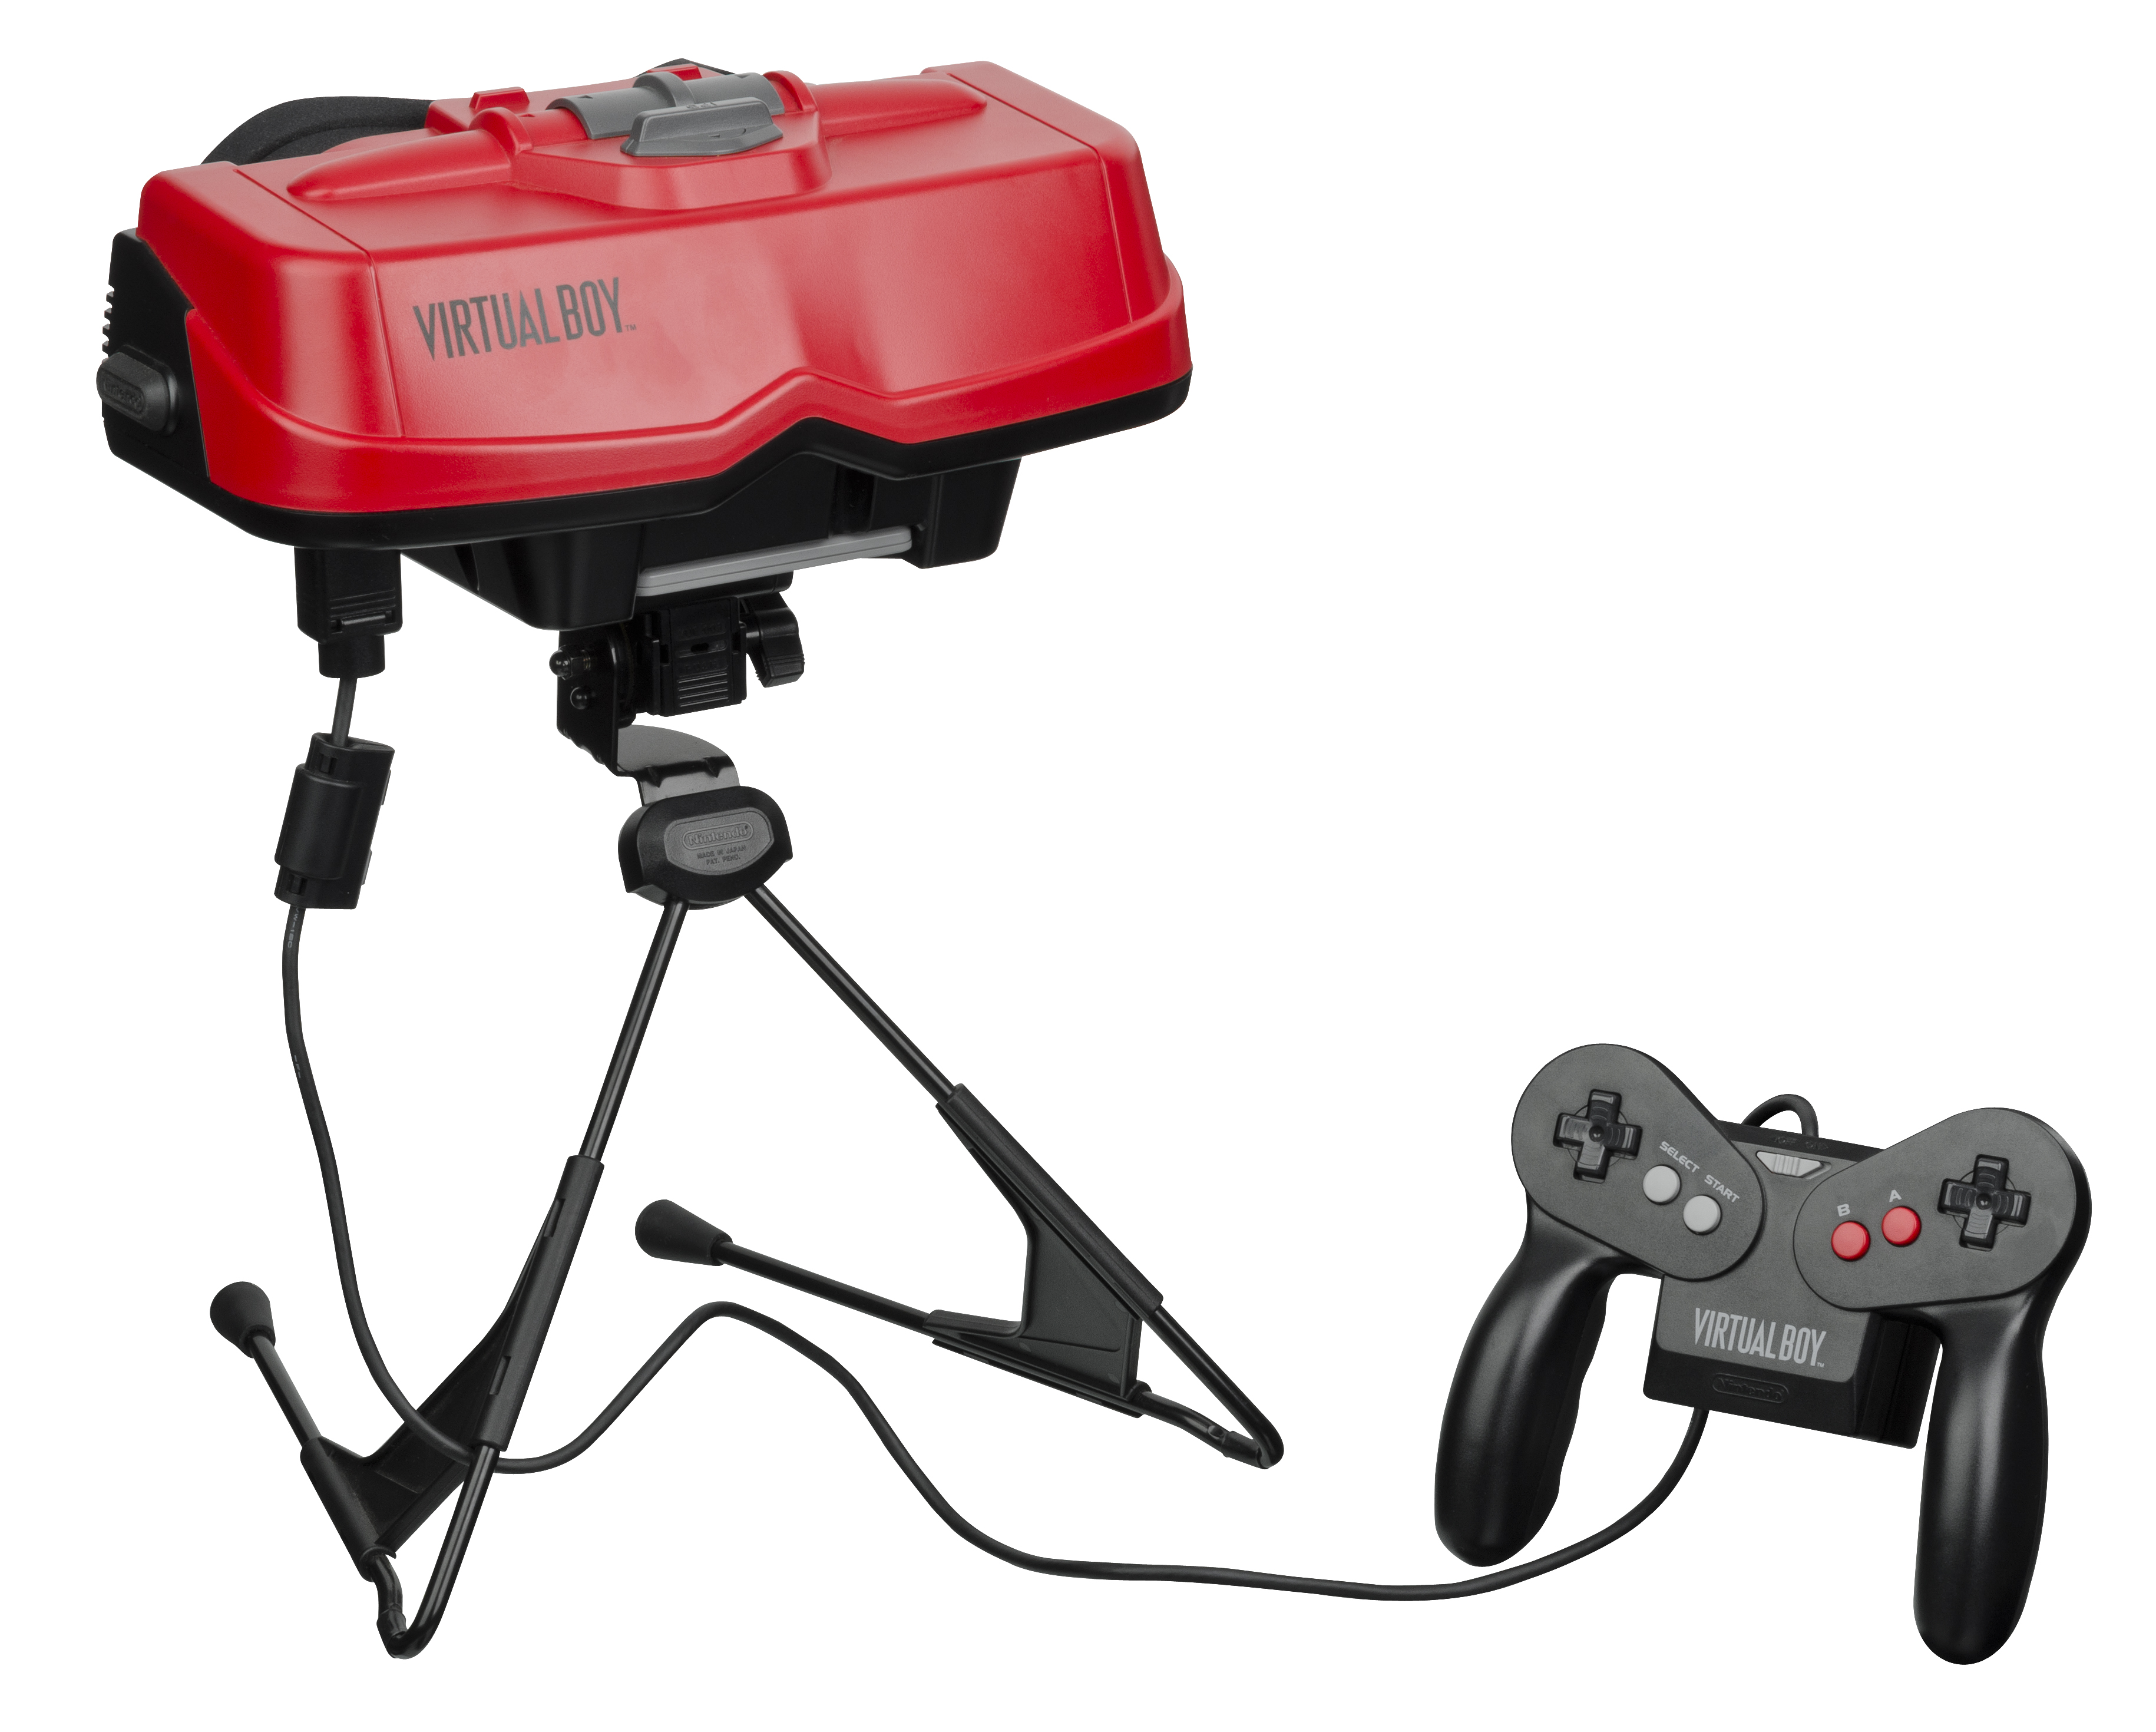
\includegraphics[width=0.5\textwidth]{images/virtualboy.jpg}
	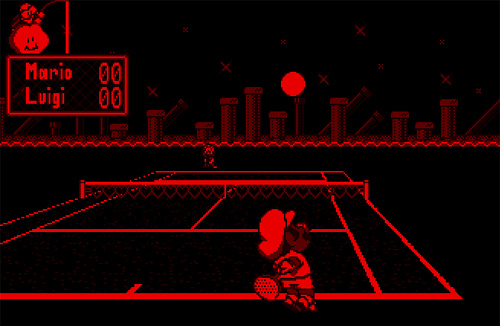
\includegraphics[width=0.5\textwidth]{images/vrmario.jpg}
  }
  \caption{Videoconsola \emph{Virtual Boy} de Nintendo Company. (1995)\\Fuente:\protect\url{https://upload.wikimedia.org/wikipedia/commons/c/ce/Virtual-Boy-wController.jpg}}
  \label{fig:virtualboy}
\end{figure}

Algunos de los dispositivos que cumplen las caracter�sticas antes mencionadas son las gafas \emph{Oculus Rift}, o su competencia las gafas \emph{HTC Vive}\citep{article:HTCVive}. Tambi�n existe su versi�n mas econ�mica para dispositivos m�viles aprovechando sus sensores de posici�n y rotaci�n. Dichas gafas empezaron con la aparici�n de las \emph{Google Cardboard}\citep{article:GoogleCardboard} en el a�o 2014. Mencionar tambi�n que el �xito de estos lanzamientos no es debido solo a su fant�stica tecnolog�a, sino tambi�n a que han proporcionado de manera libre herramientas a los programadores para el desarrollo de sus propias aplicaciones y programas.

En concreto, tanto las \emph{Oculus Rift} como las \emph{Google Cardboard} tienen a disposici�n de cualquiera y de manera gratuita un SDK para \emph{Unity 3D} que permite crear un entorno de VR.

Pero, como mencion� anteriormente, no todo gira en torno a gafas de realidad virtual basada en im�genes: existe, como ejemplo, la plataforma llamada \emph{Virtuix Omni} que nos permite desplazarnos por un mundo virtual andando o corriendo.  Consiste en una base fija en el suelo que detecta los pasos del usuario gracias a unas zapatillas especiales \citep{article:Omni}.

Otro ejemplo es el parque tem�tico llamado \emph{The Void} que recrea un escenario f�sico para adecuarlo al que se percibe en el mundo virtual a trav�s de unas gafas, introduciendo elementos como ventiladores para emular r�fagas de viento, creando as� una mayor sensaci�n de realismo al mezclar los est�mulos t�ctiles que percibimos a trav�s de nuestros sentidos \citep{www:Void}. 

En conclusi�n, la realidad virtual es una tecnolog�a que no es moderna pero que est� viviendo actualmente su �poca dorada gracias al sector del ocio. A�n as�, surgen aplicaciones para un uso con fin social, humanitario o m�dico gracias a las facilidades que hay para crear aplicaciones propias.

Dispositivos como las gafas \emph{Oculus Rift} o \emph{HTC Vive} permiten disfrutar de sensaciones nuevas llevando el ocio a un nuevo nivel y por ello su fama crece exponencialmente gracias a su coste asequible.

\lsection{Oculus Rift y otros sistemas de gafas de realidad virtual}
Las gafas de realidad virtual son los dispositivos que m�s impacto han tenido gracias a que proporcionan la mayor sensaci�n de inmersi�n: nos permiten ver un mundo distinto al nuestro. \emph{Oculus Rift} tiene el honor de ser el primer sistema HMD (\emph{Head-Mounted Display}) al despuntar en el sector gracias al uso de tecnolog�as como los giroscopios y los aceler�metros. Est� soportado por un ordenador dejando los costes computacionales de la generaci�n de gr�ficos a la tarjeta gr�fica del ordenador limit�ndose exclusivamente a mostrar im�genes y a detectar movimientos.

Aunque haya sido uno de los primeros no es el �nico. Su principal competencia son las gafas desarrolladas por \emph{Valve Corporation} y \emph{HTC Corporation} llamadas \emph{HTC Vive}. Se basan en los mismos principios y su diferencia es cuesti�n de calidad de hardware y no de funcionalidad.

Otro sector son los cascos de realidad virtual destinados a los \emph{SmartPhones}. Las primeras gafas en surgir en este sector fueron las \emph{Google Cardboard}, actualmente en su segunda versi�n. Como caracter�stica principal est�n construidas con cart�n, siendo las primeras versiones no comerciales esquemas publicados en Internet para su construcci�n casera.

Actualmente han surgido modelos m�s trabajados que sustituyen el cart�n por chasis pl�sticos. Obviamente el coste tambi�n se ve incrementado, siendo el precio de las \emph{Google Cardboard} de {5\EUR} a {10\EUR} y de otros dispositivos, como las \emph{Archos Glasses}, rondando los {25\EUR} (figura \ref{fig:vrMovil}).

\begin{figure}[h!]
  \centerline{
	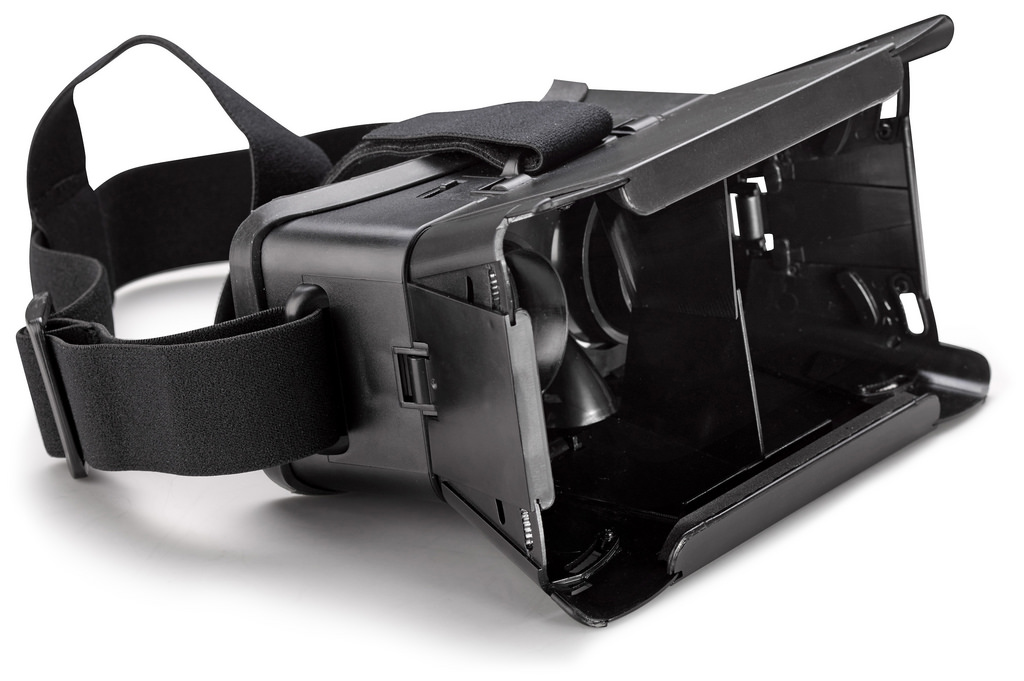
\includegraphics[width=0.3\textwidth]{images/archos.jpg}
	\includegraphics[width=0.3\textwidth]{images/gear.jpg}
	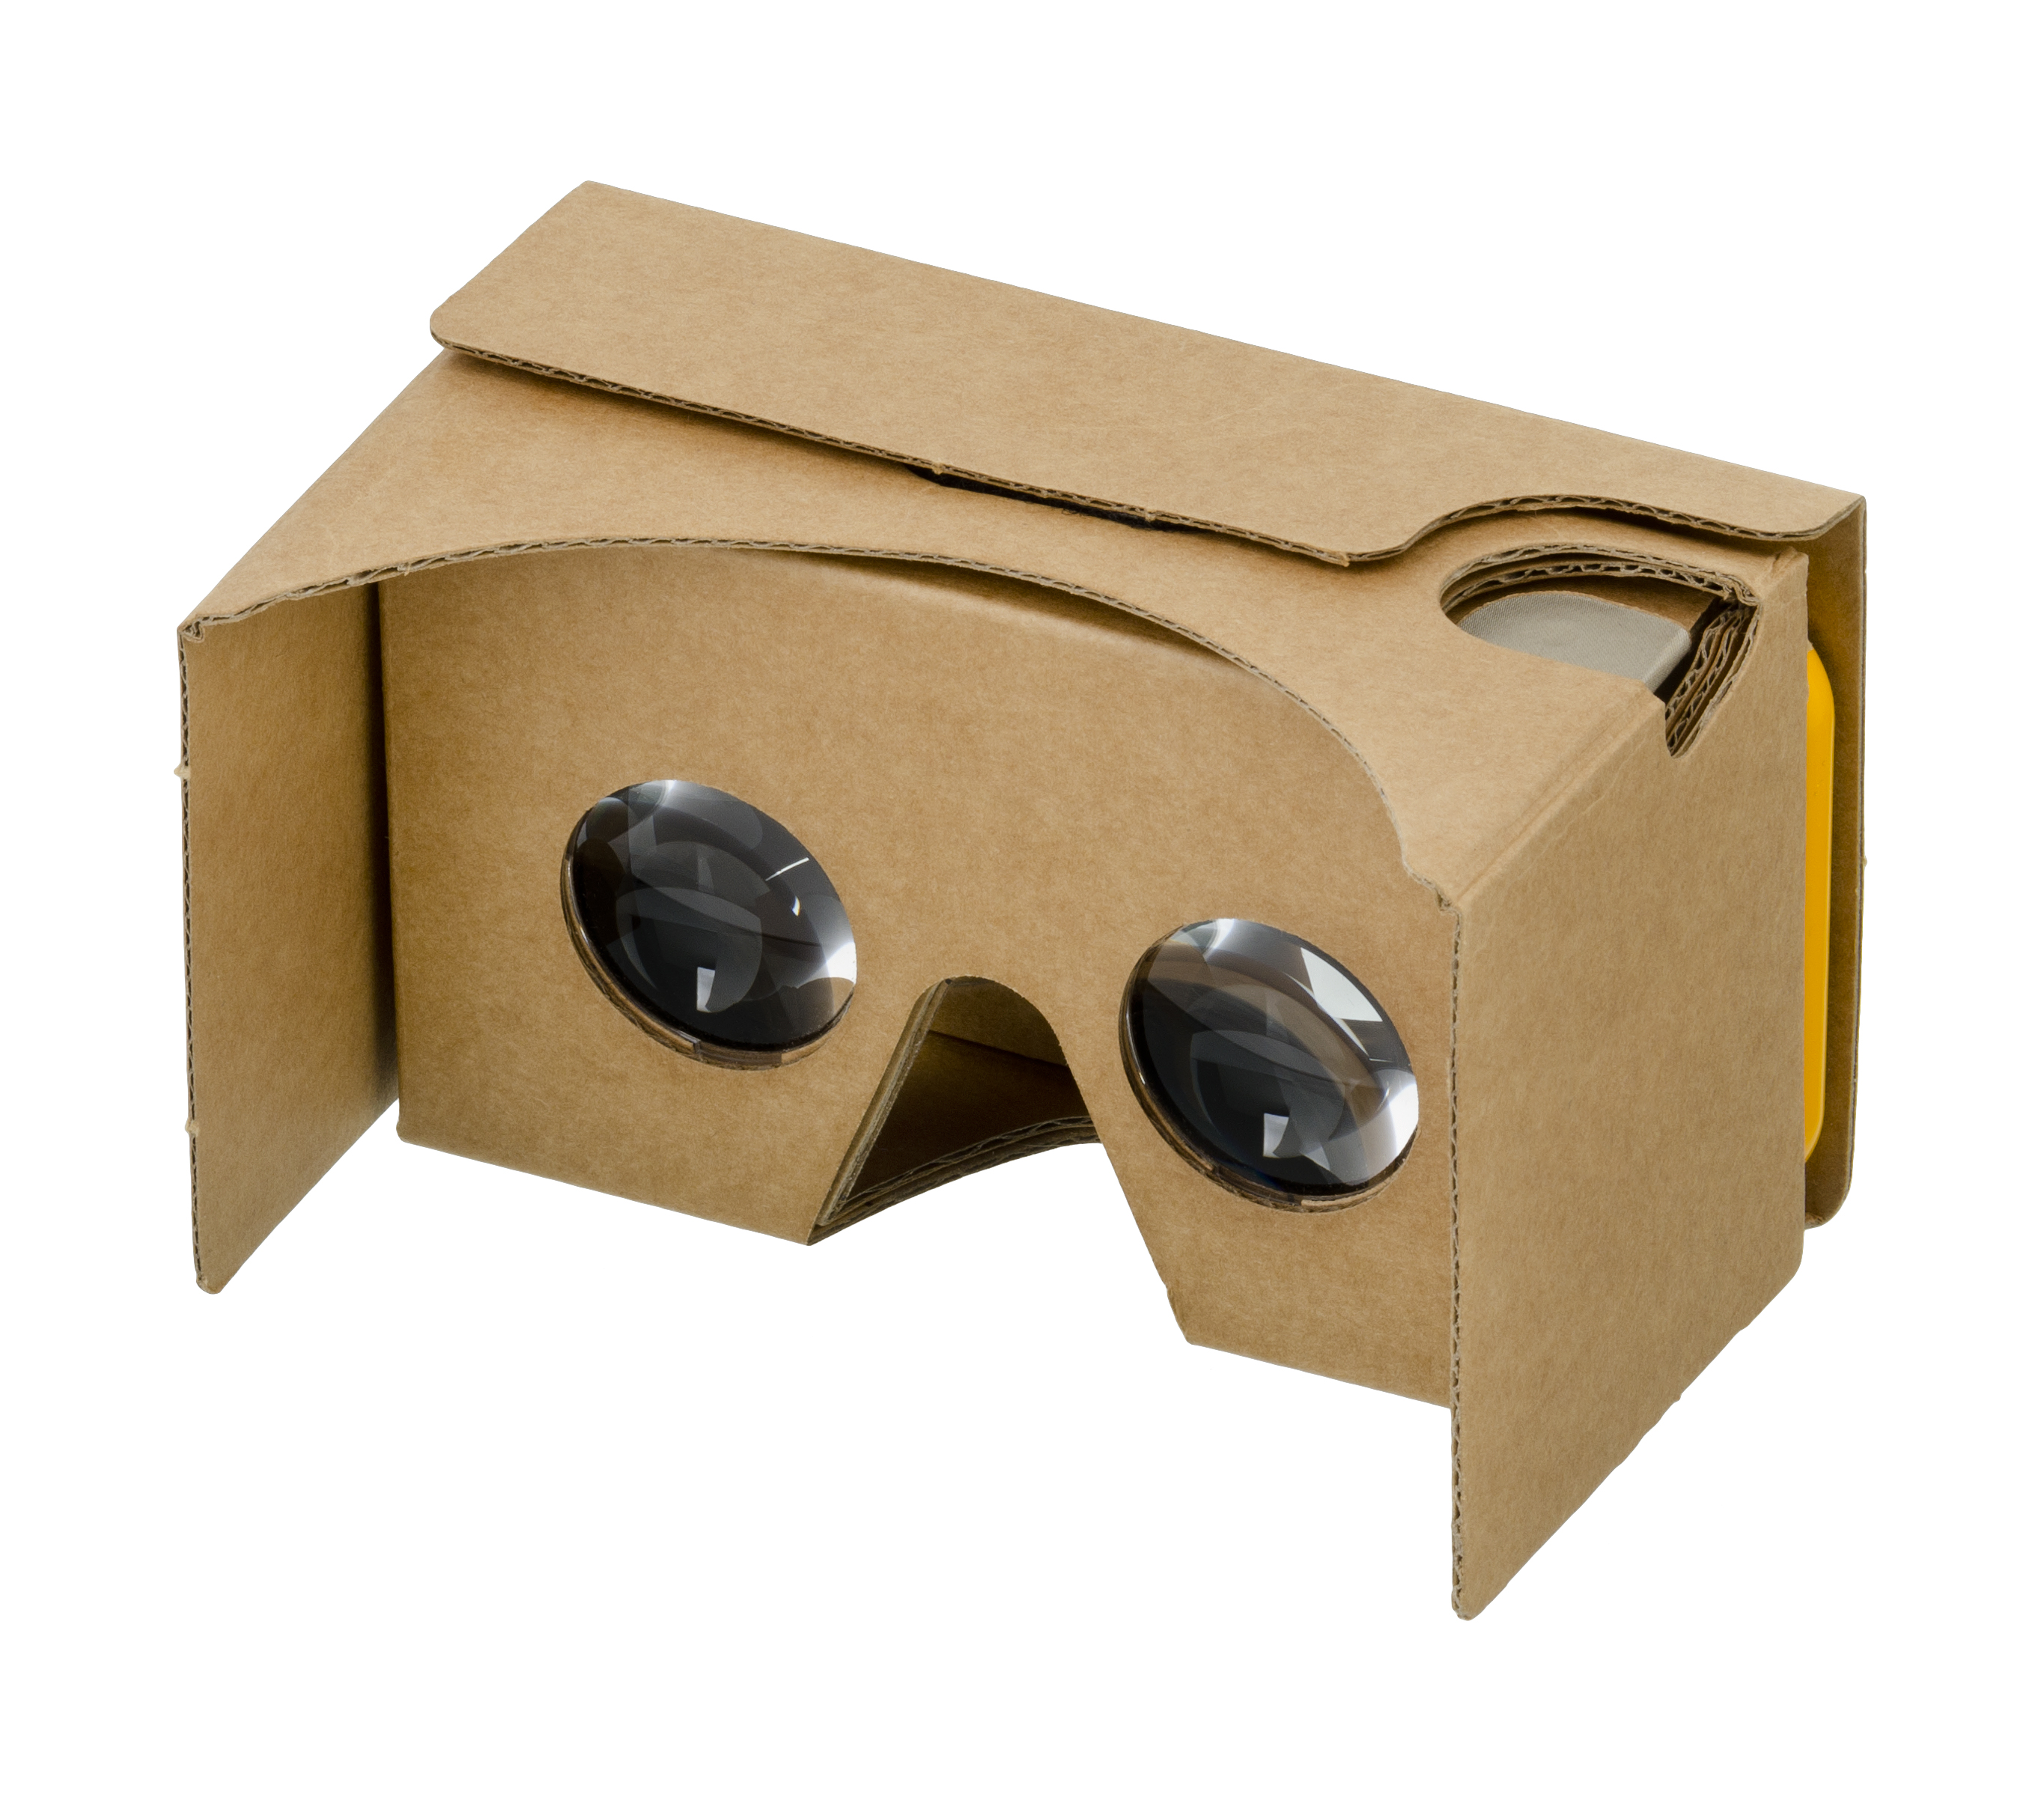
\includegraphics[width=0.3\textwidth]{images/cardboard.jpg}
  }
  \caption{\emph{Archos VR Glasses}, \emph{Samsung Gear VR} y \emph{Google Cardboard}\\Fuente:\protect\url{https://c2.staticflickr.com/6/5607/14961040484_ff7643245d_b.jpg}}
  \label{fig:vrMovil}
\end{figure}

Adem�s de lo mencionado, \emph{Oculus} ha desarrollado para \emph{Samsung} las \emph{Samsung Gear VR}, un casco de realidad virtual destinado para tel�fonos \emph{Samsung} que incorpora un touchpad con el que interaccionar. Su precio se aproxima a los {100\EUR}.

\lsection{Unity 3D}
\emph{Unity 3D} \citep{article:Unity3D} es una herramienta de dise�o e implementaci�n de videojuegos que ha revolucionado el mercado. Una de sus principales caracter�sticas es la capacidad de generar versiones para distintas plataformas como pc, videoconsolas o contenido online. Esto es gracias a que utiliza \emph{C\# / JavaScript} bajo el int�rprete \emph{Mono Runtime}. Proporciona funcionalidades para diferenciar plataformas, de modo que no hace falta generar distintos proyectos pudiendo estar la codificaci�n para distintas plataformas en un solo proyecto.


\begin{figure}
    \centering
	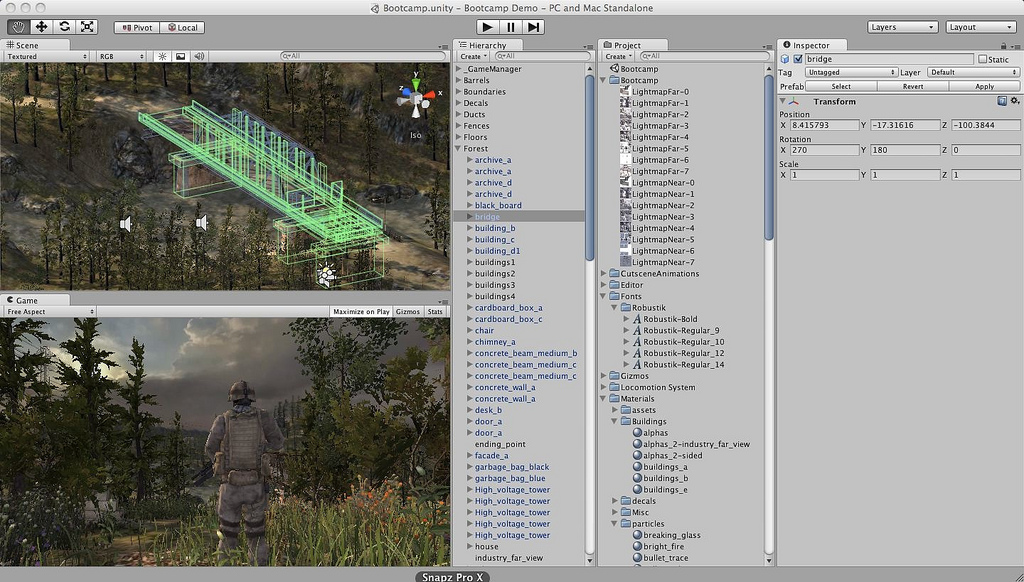
\includegraphics[width=\textwidth]{images/unity.jpg}  
  	\caption{Interfaz de usuario de \emph{Unity 3D}\\Fuente:\protect\url{https://c1.staticflickr.com/5/4130/5035620615_5891474154_b.jpg}}
  \label{fig:unity}
\end{figure}

Otra de las caracter�sticas revolucionarias es que incluye herramientas para dise�ar en 3D, generar animaciones, manejar part�culas y un motor f�sico. Antes de \emph{Unity 3D}, estas caracter�sticas se ten�an que desarrollar por separado con programas como \emph{Blender 3D} \citep{article:Blender} ,el software de modelado 3D y animaci�n de c�digo abierto.

Adem�s proporciona una tienda online donde se puede comprar u obtener gratis determinados componentes para incluirlos en nuestros juegos y aplicaciones.

Una de las desventajas con las que cuenta este software es que su curva logar�tmica de aprendizaje describe un avance lento; expresado en otras palabras, el proceso de su aprendizaje se prolonga en el tiempo debido a que la cantidad de conceptos y tecnolog�as a adquirir puede llegar a ser abrumadora. Aun as�, los desarrolladores cuentan con una colecci�n excelente de tutoriales \citep{article:UnityTutorial} en los que se esfuerzan en ayudar de manera gratuita a la comunidad. Existe tambi�n una gran cantidad de foros y sitios web donde la comunidad resuelve dudas. En Espa�a destaca la web \url{http://www.unityspain.com/}.

En conclusi�n, \emph{Unity 3D} ha llegado a ser una de las mejores tecnolog�as para el desarrollo de videojuegos adoptando una filosof�a que premia a la comunidad y da facilidades para aprender. Aunque no es un software cerrado, como toda empresa busca un beneficio econ�mico. Dicho beneficio lo consigue gracias al soporte t�cnico y al desbloqueo de herramientas, �tiles en su mayor�a cuando uno se embarca en un proyecto verdaderamente grande en \emph{Unity 3D}, con lo que no afecta al desarrollador que solo quiere aprender o hacer algo simple. Por este motivo se ha elegido como plataforma base para el desarrollo de este TFG.

\lsection{Discapacidades motoras habituales}
\label{sect:discMotoras}
Las discapacidades motoras son aquellas discapacidades que agregan una desventaja en el movimiento o en la fuerza de los movimientos de una persona. Seg�n el cuadro \ref{tabla:defMotora}, el d�ficit de fuerza se puede catalogar en seis niveles siendo el 0 la par�lisis total y el 5 el estado normal.

\begin{table}[htb]
	\centering
    \scriptsize
	\begin{tabular}{|l|l|}
		\hline
		\multicolumn{2}{|c|}{Nivel d�ficit motor} \\ \hline
		Nivel & Descripci�n \\
		\hline \hline
		0 & Par�lisis completa \\ \hline
		1 & Contracci�n muscular sin movimiento \\ \hline
		2 & Movimiento pero sin fuerza para superar la gravedad \\ \hline
		3 & Movimiento pero sin fuerza para superar una resistencia f�sica \\ \hline
		4 & Movimiento m�s d�bil del esperado\\ \hline
		5 & Fuerza normal \\ \hline
	\end{tabular}
	\caption{Cuantificaci�n del d�ficit de la fuerza motora.}
	\label{tabla:defMotora}
\end{table}

Como se ha visto, no todas las discapacidades motoras indican una imposibilidad de movimiento, sino que �nicamente pueden limitarlo. Adem�s, muchas de estas limitaciones desembocan en una atrofia muscular derivada del d�ficit de uso. 

El sistema piramidal es la v�a neuronal localizada en el sistema nervioso central que ejerce la acci�n del movimiento voluntario en el cuerpo humano. Esta orden de movimiento se genera en la corteza cerebral, donde se emplaza el n�cleo de la primera motoneurona. El ax�n (terminaci�n) de esta primera motoneurona desciende hasta la m�dula espinal donde hace contacto con la segunda motoneurona. A esta conexi�n se le llama sinapsis y es un intercambio de informaci�n por diferencias de potencial entre axones. La segunda motoneurona es la encargada de conectarse al m�sculo y generar el impulso nervioso que provoca la contracci�n de dicho m�sculo  \citep{article:CTONeuro}.

\begin{figure}[h!]
  \centerline{
	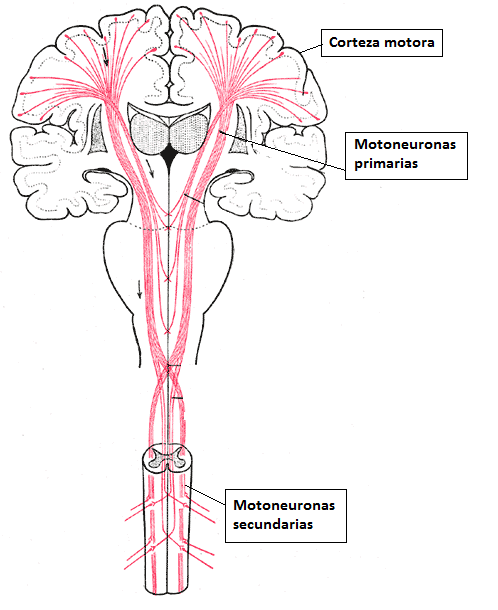
\includegraphics[width=0.6\textwidth]{images/motoneurona.png}
  }
  \caption{V�a piramidal motora.\\Fuente:\protect\url{https://upload.wikimedia.org/wikipedia/commons/6/68/Gray764.png}}
  \label{fig:viaPiramidalMotora}
\end{figure}

Las lesiones en la primera motoneurona responden a alteraciones de naturaleza diversa como problemas vasculares, isqu�micos, inflamatorios o tumorales; siendo infrecuentes las lesiones ocasionadas por traumatismos. Las manifestaciones de esta lesi�n se dan en forma de p�rdida en la precisi�n del movimiento, rigidez en extremidades, p�rdida de reflejos o combinaci�n de varias. Las lesiones en la segunda motoneurona son provocadas por los mismos motivos que la primera motoneurona sumando los traumatismos y lesiones degenerativas. Todas las lesiones en este punto producen par�lisis totales o parciales \citep{article:MPato}.

En conclusi�n, las discapacidades motoras pueden tener distinta sintomatolog�a y no se limitan solo a una imposibilidad total de movimiento. Pueden generar p�rdida de fuerza, temblores o reducci�n de la capacidad de movimiento de una extremidad. Todo esto se debe tener en cuenta a la hora de desarrollar un sistema que pretenda ayudar a este sector.

\lsection{La realidad virtual y las discapacidades}
\label{sec:RVYDisc}
Las Tecnolog�as de la Informaci�n y del Conocimiento surgen para dar soluciones a los problemas que acarrea la humanidad y por tanto es l�gico pensar que proporcionen o que al menos intenten proporcionar soluciones a las discapacidades.

Las interfaces cerebro-m�quina pueden ser una respuesta a las discapacidades motoras. Cuando nuestro cuerpo se convierte en nuestra c�rcel, nuestra mente es nuestro �nico refugio. Analizando los patrones de las ondas producidas por nuestro cerebro se puede obtener cierta informaci�n de los movimientos de una persona. Un caso de uso de esto es un estudio realizado para mover una silla de ruedas a trav�s de esta tecnolog�a en un entorno virtual. Se analizaban los patrones gracias a un casco de electroencefalogramas (EEG)\citep{article:BCISilla}. Tal vez este sea el principio de la ut�pica idea de crear un sistema para superar totalmente las discapacidades o de desarrollar una interfaz total de movimiento en entornos virtuales, como se ha visto solo en el cine. 

En el a�o 2014 se hizo un estudio en el que se evaluaba las ondas captadas por un EEG y la sensaci�n de estabilidad y equilibrio demostrando que la realidad virtual es capaz de influir en dichas sensaciones. La conclusi�n de este estudio fue que la sensaci�n de inmersi�n es lo suficientemente grande como para producir que nuestros reflejos naturales se activen por s� solos \citep{article:BCIVRCoordinacion}.

Ignorando ya las discapacidades motoras, la realidad virtual se puede usar como una herramienta m�s dentro de las TIC con el fin de ayudar a las personas. En el a�o 2015 se realiz� un estudio en el que se intentaba que pacientes con autismo adquirieran la habilidad para cruzar la calle y seguir caminos. El experimento consisti� en generar una ciudad tridimensional con tecnolog�a de realidad virtual para que personas con autismo en un rango de edad entre los 19 y los 45 a�os tuvieran que aprender y seguir un camino en el que se tienen que enfrentar a sem�foros, pasos de cebra y dem�s elementos de la vida urbana \citep{article:VRAutism}.

En conclusi�n, la realidad virtual es un campo muy prometedor que, en conjunto con otras tecnolog�as, puede dar como resultado herramientas capaces de ayudar a las personas y que merece de un esfuerzo por nuestra parte para que evolucionen. 


\newpage \thispagestyle{empty} % P�gina vac�a 

\chapter{Sistema, dise�o y desarrollo}
\label{chap:sistemadesarrollado}
En este cap�tulo se exponen las labores desarrolladas en este TFG. Para ello, primero hay que entender en detalle las tecnolog�as implicadas en su desarrollo: \emph{Oculus Rift} y \emph{Unity 3D}. Despu�s se pasa a la parte de dise�o y desarrollo del software, para ello hay una descripci�n de los requisitos funcionales y no funcionales subcatalogados en \emph{Fundamentales} (cuyo objetivo es este TFG) o \emph{No Fundamentales} cuyo desarrollo se pospondr� a un trabajo futuro. Se mostrar� a continuaci�n el dise�o de clases a trav�s de un diagrama de clases de la aplicaci�n y los distintos escenarios de casos de uso del sistema.

\lsection{Oculus Rift}

En esta secci�n nos centraremos en las \emph{Oculus Rift} m�s en profundidad. Hay que tener en cuenta que muchos de sus principios b�sicos de funcionamiento los comparte con otros dispositivos como las \emph{HTC Vive} o las \emph{Google Cardboard}.

\subsection{Aspectos F�sicos}
El principal principio en el que se basan las \emph{Oculus Rift}, y casi todos los sistemas de realidad virtual enfocados al sentido de la vista, es en la capacidad de nuestro cerebro para fusionar im�genes cuando se presentan por individual en cada ojo. El impedimento que esto conlleva es que usuarios con enfermedades como el estrabismo ocular tienen dificultades para realizar dicha fusi�n. En consecuencia, tienen problemas en la percepci�n de la profundidad y en el caso de uso de tecnolog�as 3D (no solo las enfocadas a la realidad virtual) pueden sufrir mareos e incapacidad para percibir la formaci�n de la imagen 3D, ya que solo ser�n capaces de ver figuras borrosas, de manera similar a cuando nos quitamos las gafas en un cine 3D.

Este principio se basa en la convergencia ocular y en el �ngulo de convergencia que forman los dos ojos con el objeto que se percibe. Imaginemos un objeto situado frente a nosotros: debido a que disponemos de una visi�n binocular (cada ojo ve el objeto por separado) la focalizaci�n de este objeto percibido requiere del posicionamiento de cada ojo en un �ngulo adecuado, de modo que ambas im�genes convergir�n y se percibir�n como una sola y con una profundidad adecuada respecto al espacio que le rodea. El �ngulo de convergencia que forman los dos ojos con el objeto que se percibe aumenta a medida que el objeto se halla m�s pr�ximo y disminuye cuando el objeto est� m�s lejano. Esta distancia de convergencia suele estar en un valor entre 7 y 11 cm. Cuando el �ngulo o distancia de convergencia no es adecuado se produce la llamada diplopia o visi�n doble, que explica porqu� cuando acercamos mucho a la nariz un objeto, la imagen no se forma correctamente en nuestro cerebro y la vemos borrosa.

En la figura \ref{fig:fusionojos} se puede ver un peque�o esquema en el que se ha representado el �ngulo de convergencia de cada ojo y c�mo se produce la fusi�n (3D) cuando se posiciona a la distancia adecuada. 

\begin{figure}[H]
    \centering
	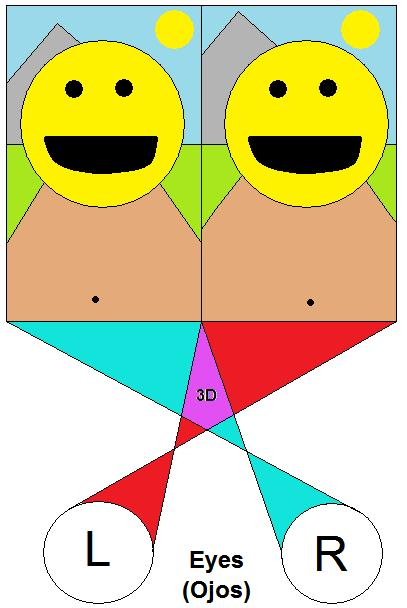
\includegraphics[width=0.5\textwidth]{images/distanciafusion.png}
  
  \caption{Diagrama que representa como las im�genes percibidas por nuestros ojos fusionan una imagen.\\Fuente:\protect\url{https://es.wikipedia.org/wiki/Estereoscopia\#/media/File:Estereoglifo.jpg}}
  \label{fig:fusionojos}
\end{figure}

El problema de un sistema de gafas de realidad virtual es que no es capaz de proporcionar una imagen a una distancia de convergencia adecuada, debido a que esta distancia de la que habl�bamos anteriormente es de aproximadamente 10 cm, por lo que har�a necesario dise�ar unas gafas de profundidad excesiva. Para dar soluci�n a este problema se ha ideado un sistema en el que se generan las dos im�genes con una serie de trasformaciones afines pertinentes, de modo que sea posible corregir esta distorsi�n provocada por la poca profundidad de las gafas. Adem�s se utilizan unas lentes capaces de aumentar la imagen para que el ojo las perciba adecuadamente y se produzca la fusi�n y la percepci�n del mundo 3D. A este tipo de im�genes se las conoce como im�genes estereosc�picas \citep{article:Estereoscop�a}. El concepto de imagen estereosc�pica no es actual sino que surgi� hace tiempo, existiendo juguetes con estas im�genes que datan del siglo anterior.

\subsection{Hardware}
El hardware que se va a describir a continuaci�n es el correspondiente a las \emph{Oculus Rift Development Kit 2 (DK2)}, que concierne a la versi�n con la que se ha trabajado. Actualmente existe una nueva versi�n comercial, de manera que esta versi�n ha quedado obsoleta. Las diferencias principales con sus rivales como las \emph{HTC Vive} son las caracter�sticas HW que las definen, es decir, tama�o de pantalla, calidad de �sta, etc.

\subsubsection{Pantalla}
Para representar las im�genes con las que trabaja cuentan con una pantalla con una resoluci�n de 1980x1080 con una latencia de imagen en el rango de los [2,3] ms, lo que garantiza una velocidad de refresco de imagen casi en tiempo real. En la versi�n DK1, el alto tiempo de latencia provocaba el llamado efecto \emph{Judder} que consiste en un desfase de la se�al de audio y v�deo. Basada en la tecnolog�a OLED \cite{wiki:OLED}, se consigue eliminar el efecto \emph{Judder} \citep{article:WikiJudder} y el llamado \emph{Motion Blur} \citep{article:WikiBlur} que tiene lugar en im�genes o v�deos en los que aparece un movimiento r�pido.

\begin{figure}[h!]
  \centerline{
	\includegraphics[width=0.5\textwidth]{images/motionblur.jpg}
	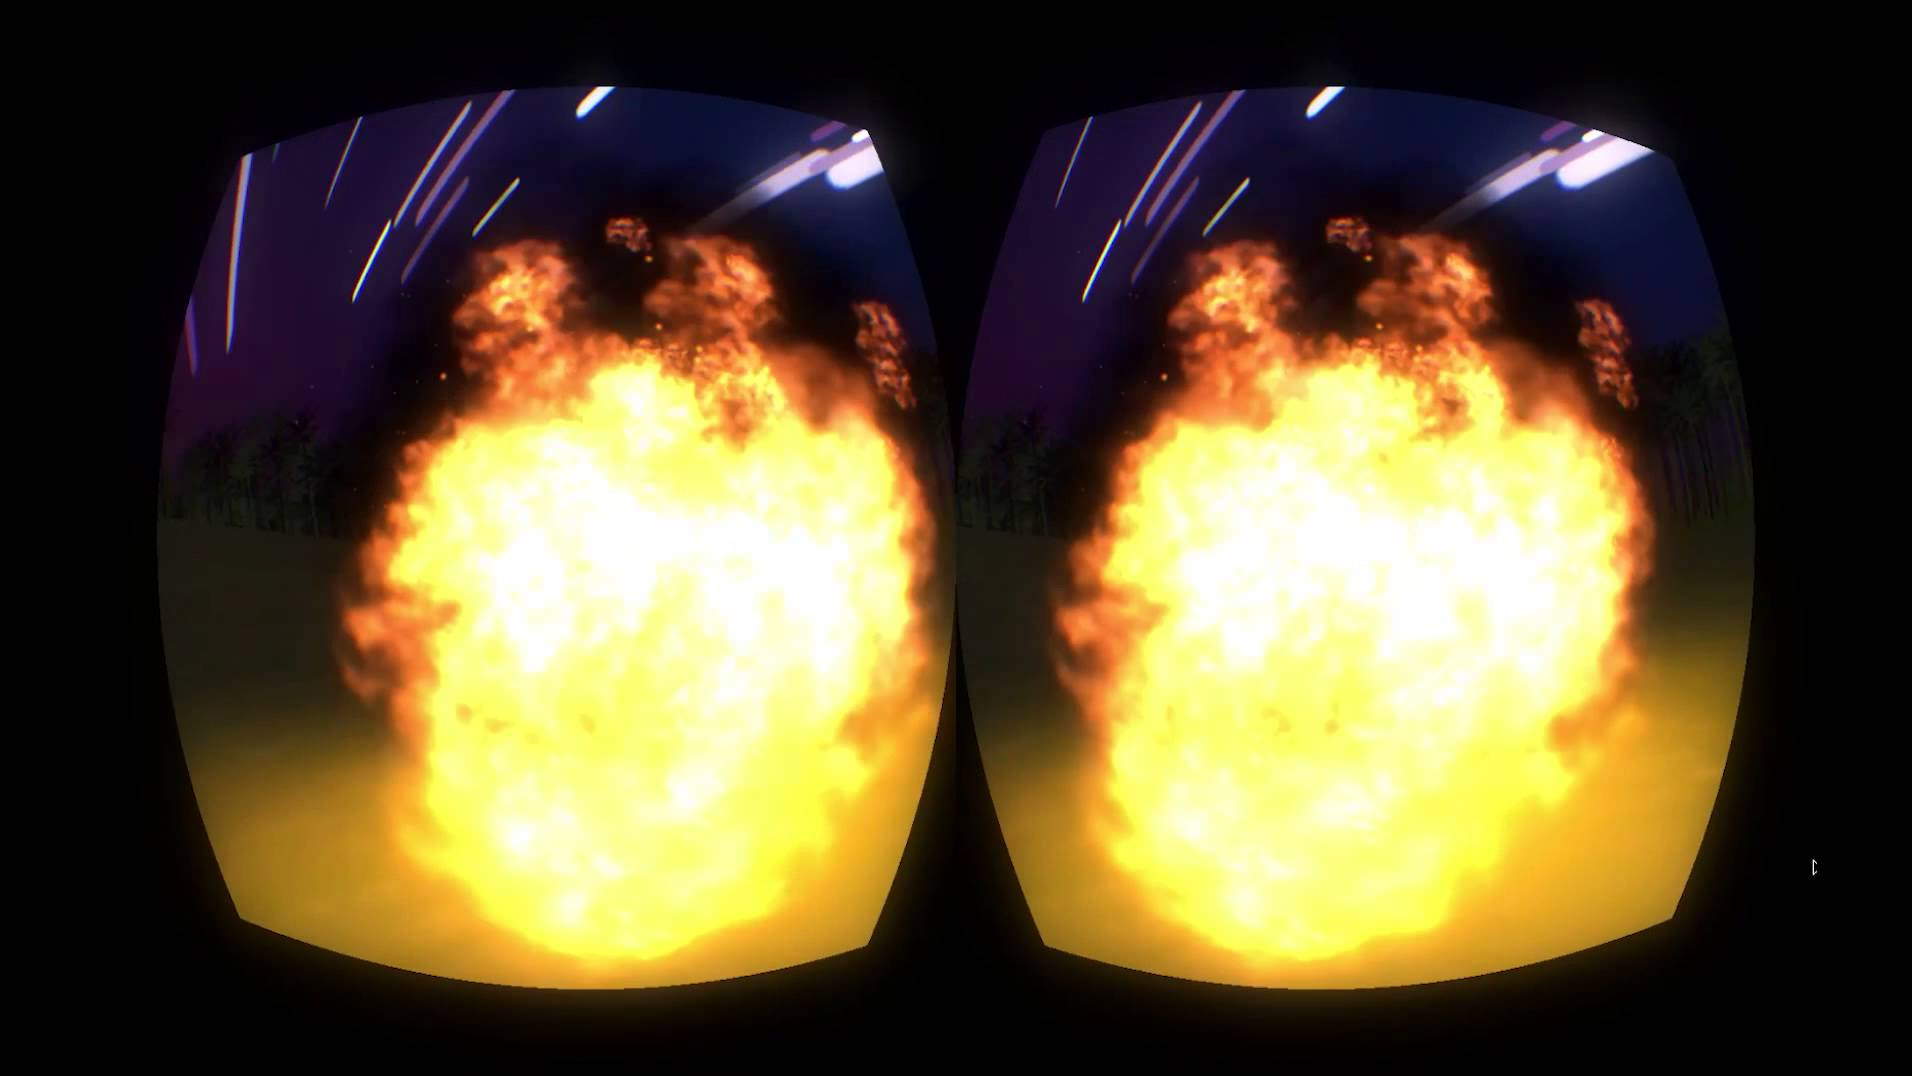
\includegraphics[width=0.5\textwidth]{images/imgdk2.jpg}
   }
	\caption{Efecto \emph{Motion Blur} en un autob�s y pantalla de la versi�n DK2.\\Fuente:\protect\url{https://upload.wikimedia.org/wikipedia/commons/2/26/London_bus_and_telephone_box_on_Haymarket.jpg}}
 	\label{fig:motionblur}
\end{figure}


Para la conexi�n con el ordenador se utiliza un conector tipo HDMI, lo que permite que en el frontal de las gafas haya un conector Jack de audio. El audio es una se�al que se manda junto con el video por un canal HDMI.


\subsubsection{Giroscopio y acelerometro}
La base de todas las gafas de realidad virtual es la capacidad de detecci�n de los movimientos rotacionales de la cabeza junto con el movimiento acorde de la c�mara dentro del mundo tridimensional. Hablando exclusivamente de rotaciones, un objeto puede rotar �nicamente en torno a tres vectores, ejemplificado en la figura \ref{fig:rotObjets}. Para poder implementar esta funcionalidad, \emph{Oculus Rift} cuenta con un giroscopio de tres ejes y un aceler�metro. As� calcula la direcci�n de rotaci�n y aceleraci�n del movimiento. Gracias a que los \emph{Smartphones} actuales tambi�n tienen estos dispositivos, existen gafas como las \emph{Google Cardboard}.

\begin{figure}[ht!]
  \centerline{
	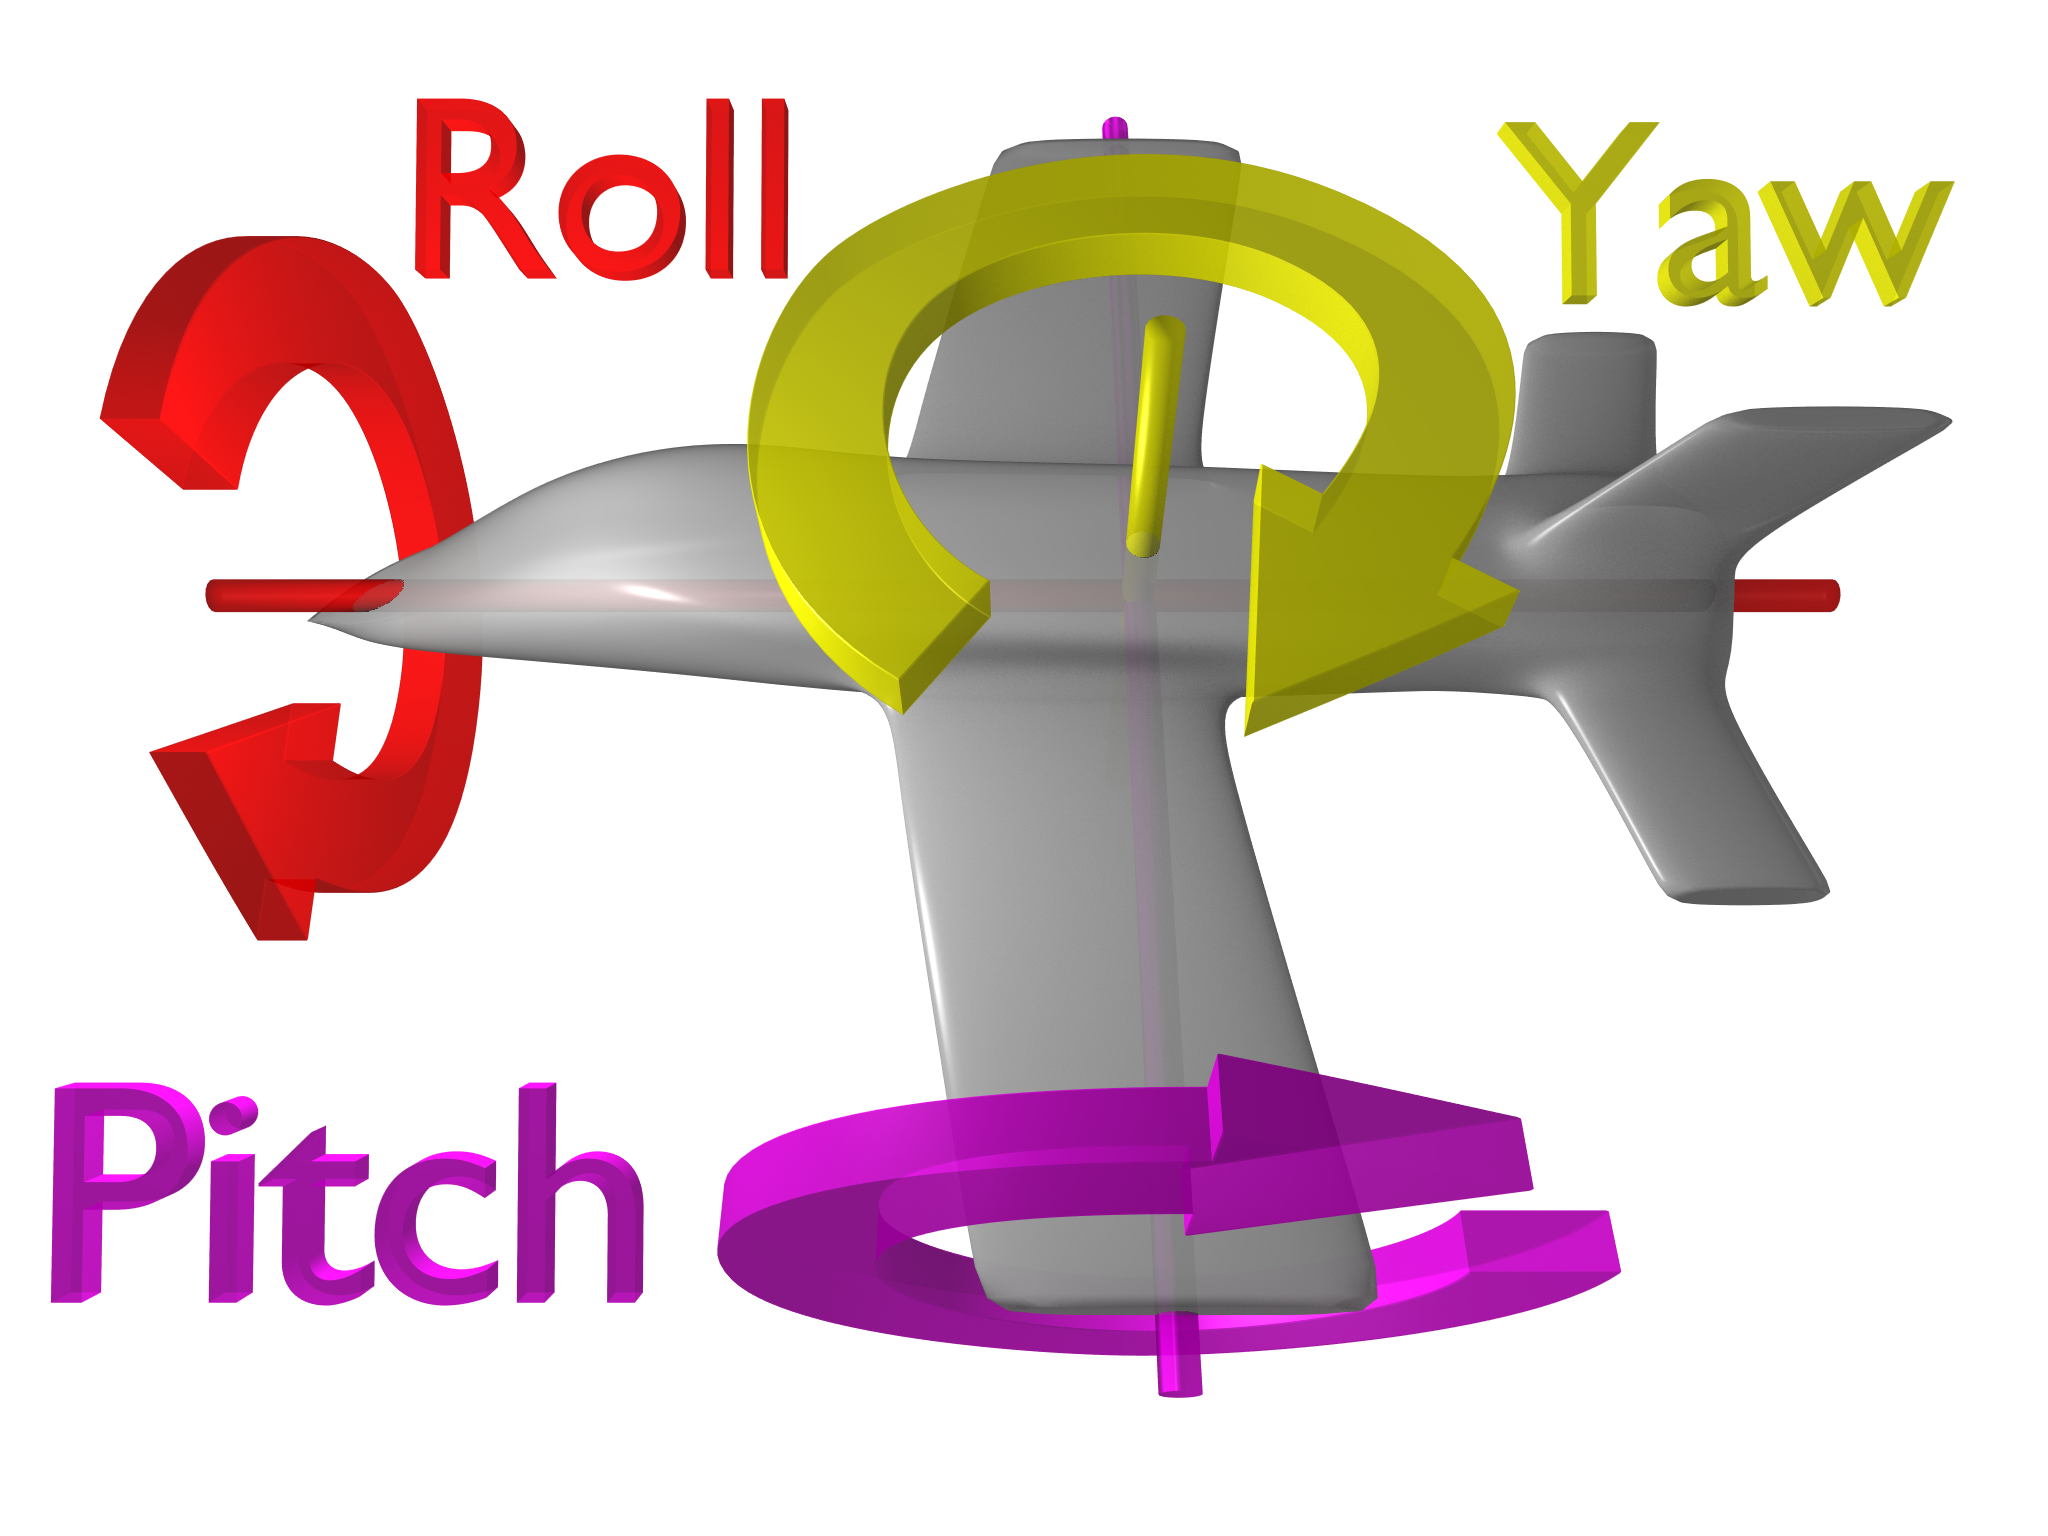
\includegraphics[width=0.5\textwidth]{images/ryp}
  }
  \caption{Ejemplo de rotaciones posibles sobre un objeto, en este caso un avi�n.\\Fuente:\protect\url{https://upload.wikimedia.org/wikipedia/commons/5/54/Flight_dynamics_with_text.png}}
  \label{fig:rotObjets}
\end{figure}

\subsubsection{Sensor Infrarrojos}
Una de las mejoras sobre la versi�n DK1 es la incorporaci�n de emisores de infrarrojos en la carcasa de las gafas, lo que permite que un sensor que se asemeja mucho a una c�mara, figura \ref{fig:dk2sinfra} , detecte los movimientos de una persona relacionados con la profundidad. Es decir, el usuario puede acercarse, alejarse, inclinarse a la izquierda o a la derecha y el sistema lo detectar�. Esto es una mejora asombrosa, pues genera mucha m�s libertad de movimiento y nos permite introducirnos m�s en los espacios tridimensionales.

\begin{figure}[ht!]
  \centerline{
	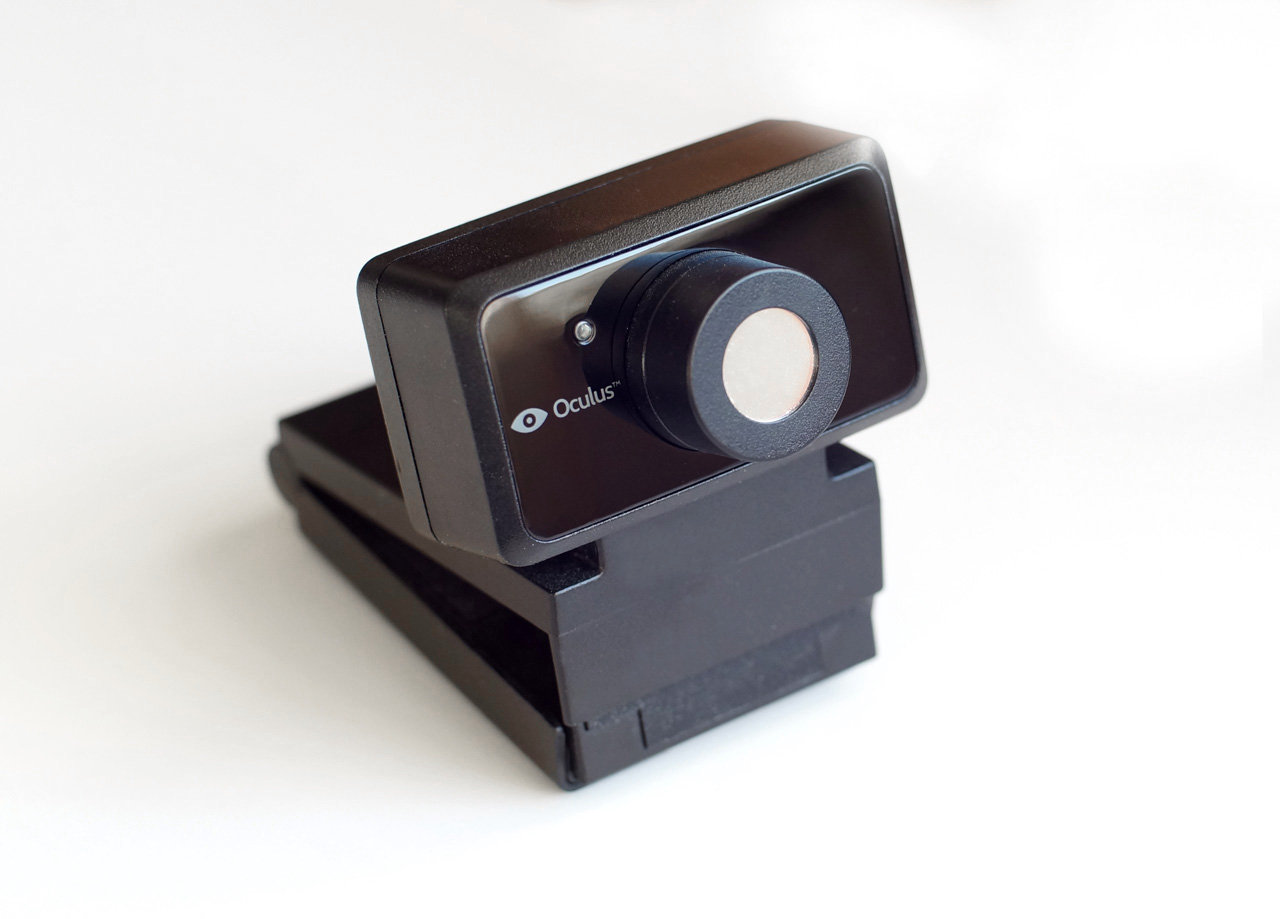
\includegraphics[width=0.5\textwidth]{images/sensorInfra.jpg}
  }
  \caption{Sensor de infrarrojos de la versi�n DK2.\\Fuente:\protect\url{https://upload.wikimedia.org/wikipedia/commons/9/9c/Oculus_Rift_Development_kit_2_positional_tracker.jpg}}
  \label{fig:dk2sinfra}
\end{figure}

\subsubsection{Dependencias de hardware}
Como ya se ha mencionado antes, las \emph{Oculus Rift/HTC Vive} son dependientes de un ordenador. Tienen conexi�n HDMI para acceder a la tarjeta gr�fica de un ordenador. En realidad son casi como un monitor extra. Casi por que hasta hace no mucho, para determinados juegos, se daba soporte a estos dispositivos configurando las gafas como un monitor externo, aunque de eso se hablar� en m�s detalle en secciones siguientes. 

Por este motivo, se requiere de un ordenador medianamente potente para su uso, hecho que genera un coste econ�mico oculto. Este TFG se ha desarrollado con un ordenador con las caracter�sticas recomendadas por \emph{Oculus Rift}. 

Estas caracter�sticas son:
\begin{itemize}
\item Procesador Intel I7 a 3.2Ghz.
\item 16 Gb de Memoria RAM DDR5.
\item T.Gr�fica \emph{Nvidia GeForce 970X} con 5 Gb DDR5.
\item HDD 1Tb rotatorio.
\item Windows 8.1
\end{itemize}

Los requisitos m�nimos de este dispositivo son:
\begin{itemize}
\item Procesador Intel I5-4590 o similar
\item 8 Gb de Memoria RAM.
\item T.Gr�fica \emph{Nvidia GTX 600 serie \ AMD Radeon HD 7000 series}.
\item Windows 7
\end{itemize}

\subsection{Software}

Para desarrollar con las \emph{Oculus Rift DK2} el fabricante incluye un SDK bastante completo que proporciona acceso a sus sensores, as� como herramientas ya creadas para que el desarrollo sea lo m�s modular posible. A parte de las descritas a continuaci�n, tambi�n existen herramientas para el desarrollo de las \emph{Samsung Gear VR}, unas gafas de realidad virtual para m�viles creadas por la compa��a para \emph{Samsung}.

\subsubsection{SDK y Runtime}
Este m�dulo es el m�dulo b�sico que se debe instalar para usar el dispositivo. Contiene los drivers y librer�as necesarias para dar soporte \citep{www:OculusDescargas} :

\begin{itemize}
\item \textbf{Oculus Audio SDK} para dar soporte a la tecnolog�a VST para el tratamiento y procesamiento de audio \citep{wiki:VST} y a�adir efectos de audio para obtener m�s sensaci�n de inmersi�n. Un ejemplo de esto ser�a que, si giramos la cabeza y ponemos un o�do m�s cerca de la fuente que el otro, el sistema detecta este hecho y aumenta el volumen del canal est�reo correspondiente.
\item \textbf{Oculus Platform SDK} para el soporte del motor gr�fico y de videojuegos \emph{Unreal Engine}.
\item \textbf{Oculus PC SDK} proporciona drivers b�sicos as� como ejemplos y herramientas para \emph{Windows}. Existe tambi�n un hilo paralelo para \emph{OS X} y antiguamente tambi�n para distribuciones \emph{Linux} pero fue retirado cuando \emph{Unity 3D} quit� su soporte para dicho SO. Con el runtime se puede desarrollar en \emph{C++} sin necesidad de un editor de videojuegos.
\end{itemize}

\subsubsection{Herramientas para desarrollo}
Esta secci�n se compone de las herramientas y SDK's para desarrollar videojuegos en \emph{Unity 3D} y \emph{Unreal Engine}.

\begin{itemize}
\item \textbf{Unreal Engine 4 Integration} para dar soporte a \emph{Unreal Engine 4}.
\item \textbf{Oculus Utilities for Unity 5} para dar soporte a \emph{Unity 3D}.
\end{itemize}

\subsection{Configuraci�n del DK2}
Para desarrollar con el modelo \emph{DK2} primero el usuario debe ajustarse las gafas de manera personal. Dentro del software b�sico de drivers, hay un editor de perfil que  permite crear y guardar ajustes para cada usuario del dispositivo. Los datos que se guardan son los siguientes:

\begin{itemize}
	\item \textbf{Distancia entre ojos:} Se calcula la distancia entre el centro del iris de cada ojo. Este es un valor necesario para el c�lculo de las distorsiones a generar para obtener la fusi�n de im�genes. Un mal ajuste hace que veamos borroso el mundo virtual. El propio gestor de perfiles tiene una funcionalidad de test en la que se nos hace una prueba para que se autoajuste este valor.
	\item \textbf{Altura del cuello respecto al hombro:} Como se ha comentado, \emph{Oculus Rift DK2} incluye un sensor de posici�n. Este par�metro es un ajuste para dicho sensor.
	\item \textbf{Altura del usuario:} Este par�metro tiene la misma finalidad y complementa al de la altura del cuello. 
\end{itemize}

Adem�s de los mencionados anteriormente tambi�n se almacena el nombre del perfil, el genero y la edad de dicho usuario.

Por otro lado se cuenta tambi�n con dos tipos de lentes distintas: las lentes de tipo A est�n pensadas para personas que no tienen ning�n tipo de problema visual mientras que las de tipo B est�n pensadas para lo contrario. Una de las limitaciones de estas lentes es que las lentes de tipo B generalizan, pudiendo haber muchas combinaciones distintas de defectos oculares que se solucionen con las lentes adecuadas. Una idea de futuro podr�a ser que en las �pticas se pudieran personalizar dichas lentes.

\lsection{Unity 3D}
\emph{Unity 3D} es un software de creaci�n de videojuegos que sigue una filosof�a multiplataforma. Dan soporte a casi todos los sistemas actuales: \emph{Linux, OS X, Windows, Android, iOS, Tizen, PlayStation 4} y muchos otros. Por este motivo y por la existencia de un SDK de \emph{Oculus Rift} se ha elegido esta herramienta para desarrollo del TFG. 

\emph{Unity 3D} incluye herramientas para a�adir publicidad, hacer an�lisis estad�sticos sobre los jugadores, crear plataformas multijugador y utilizar sistemas de control de versiones. Muchas de estas caracter�sticas se desbloquean al comprar la licencia de uso comercial. En este caso, se ha usado la versi�n libre, por lo que muchas de estas herramientas no est�n incluidas.

A continuaci�n se explican algunas de las caracter�sticas m�s importantes de  \emph{Unity 3D}.

\subsection{C\#, JavaScript y Mono Runtime}

Para el desarrollo de c�digo se usa \emph{C\#} y \emph{JavaScript} que se interpreta en \emph{Mono Runtime}. Este es el secreto de su capacidad multiplataforma. No existe diferencia en las funcionalidades que aporta cada lenguaje a nivel de \emph{Unity 3D}, siendo a gusto del programador el uso de uno u otro. Se aconseja, por otro lado, el uso de \emph{JavScript} para la creaci�n de funcionalidades simples y de f�cil dise�o, dejando el resto a  \emph{C\#}.

\emph{C\#} tiene varias ventajas, entre la que se encuentra que es un lenguaje tipado y no tipado. Es decir, tiene clases y tipos de datos b�sicos como int, string, double, etc. Tambi�n posee un tipo gen�rico que permite una programaci�n no tipada. Dicho tipo de dato se usa haciendo declaraciones con la palabra reservada \emph{var}. \emph{C\#} es un lenguaje parecido a \emph{Java} desde el punto de vista de que se ejecuta sobre una m�quina virtual que traduce a c�digo m�quina. La m�quina virtual se llama \emph{Common Language Runtime}(CLR) y admite m�s lenguajes como \emph{F\#} permitiendo crear proyectos mixtos. \emph{Unity 3D} utiliza \emph{Mono Runtime} que es la versi�n open source de CLR. \emph{Mono Runtime}\citep{article:MonoRuntime} es un interprete que se encarga del manejo de las llamadas a sistema operativo y de la ejecuci�n del c�digo. Maneja la memoria de los programas y su liberaci�n a trav�s del \emph{Garbage Collector}. \emph{C\#} es un lenguaje con orientaci�n a objetos que incluye la caracter�stica de la \emph{Herencia M�ltiple}, que permite que una clase obtenga propiedades de m�s de un tipo distinto de clase padre.

Dado que utiliza \emph{Mono Runtime}, se puede usar el IDE \emph{Mono} para programar, siendo este el predilecto en \emph{OS X}, aunque se potencia m�s el uso de \emph{Visual Studio}, el IDE predilecto de \emph{Windows}. Uno de los defectos de \emph{Visual Studio} es su tama�o, ya que llega a los 20 Gb debido a que incorpora herramientas para desarrollar con el framework \emph{Windows Forms} y Xamarin Forms. Por ese motivo se ha elegido como IDE \emph{Mono}.

\subsection{Descripci�n de Unity 3D}
A continuaci�n se describir� el uso y caracter�sticas del desarrollo y programaci�n con \emph{Unity 3D} que es el software con el que se ha gestionado y creado este trabajo.

\subsubsection{Elementos Gr�ficos: GameObjects y escenas}
La clase GameObject \citep{www:UnityGameObject} es la clase base de todo elemento gr�fico de \emph{Unity 3D}. Incluye funciones para instanciarlo, destruirlo, generar transformaciones sobre �l u obtener referencia sobre GameObjects similares. Tambi�n puede contener en su interior otros GameObjects. Un elemento 2D que represente un bot�n o un panel sobre el que dibujar tambi�n es un GameObject.

Los GameObjects se instancian en lo denominado escena. Una escena es una representaci�n tridimensional en primer lugar del espacio donde se va a representar el juego. Para juegos en 2D tambi�n se usan escenas solo que se juega con las c�maras para que no tenga efecto 3D.

Todo conjunto de GameObjects puede guardase en una plantilla para poder reutilizar m�s adelante. Dichas plantillas se llaman Prefabs y est�n creadas para realizar un uso y dise�o modular de todos los objetos que creemos. Para incorporarlo al juego solo tenemos que pinchar en �l en la ventana de assets y arrastrarlo a la posici�n que deseemos dentro de la escena. 

Parte del SDK de \emph{Oculus Rift} para \emph{Unity 3D} est� compuesto de Prefabs que permiten usar el dispositivo con algo tan simple como arrastrar un Prefab a la escena del juego con la que estamos trabajando. En concreto, uno de los Prefabs m�s �tiles que tiene es el de la c�mara que ya genera las distorsiones adecuadas para crear im�genes estereosc�picas.

\subsubsection{Clase base de control: MonoBehaviour}
La clase MonoBehaviour \citep{www:UnityMonobehaviour} proporciona acceso al ciclo de vida que tiene un script (c�digo a ejecutar en una escena) dentro de un GameObject. Similar al ciclo de vida de una aplicaci�n de \emph{Android}. Proporciona un m�todo para inicializar variables y atributos, para liberar recursos, y para ejecutar acciones en cada frame (unidad de refresco de imagen) del juego. Tambi�n proporciona acceso a funcionalidades de \emph{Unity 3D} como la instanciaci�n de GameObjects. 

El orden de ejecuci�n, de primero a �ltimo, es el que se muestra a continuaci�n. De cada apartado se muestran los m�s relevantes, pues puede llegar a haber varias rutinas por apartado:

\begin{itemize}

\item \textbf{Editor}
\begin{itemize}
\item \textsl{Reset} Es el m�todo que se invoca cuando el c�digo es a�adido al GameObject.
\end{itemize}

\item \textbf{Cuando carga la primera escena}
\begin{itemize}
\item \textsl{OnLevelWasLoaded} Es el m�todo que se invoca cuando la nueva escena o nivel ha sido cargado. 
\end{itemize}

\item \textbf{Antes de la actualizaci�n del primer frame}
\begin{itemize}
\item \textsl{Start} Start es llamado antes de la primera actualizaci�n de frame solo si la instancia del script est� activada.
\end{itemize}

\item \textbf{Entre frames}
\begin{itemize}
\item \textsl{OnApplicationPause} Es el m�todo que se invoca cuando se pausa la escena
\end{itemize}

\item \textbf{Orden de actualizaci�n}
\begin{itemize}
\item \textsl{FixedUpdate} Es el m�todo que se invoca cuando los frames por segundo (FPS) son demasiado bajos.
\item \textsl{Update} Es el m�todo que se invoca una vez por frame. En esta funci�n se hacen c�lculos de movimientos o l�gica b�sica de movimiento.
\item \textsl{LateUpdate} Es el m�todo que se invoca justo despu�s de Update. Se suele usar en c�maras de tercera persona o similar.
\end{itemize}

\item \textbf{Renderizado}
\begin{itemize}
\item \textsl{OnGUI} Es el m�todo que se invoca cuando ocurre un evento en interfaz gr�fica. Dicho evento no tiene porqu� ser siempre de tipo input.
\end{itemize}

\item \textbf{Corrutinas}
\begin{itemize}
\item \textsl{yield} Se ejecuta cuando no hay m�s objetos a los que invocar la funci�n Update.
\end{itemize}

\item \textbf{Cuando el objeto es destruido}
\begin{itemize}
\item \textsl{OnDestroy} Es el m�todo que se invoca cuando el objeto va a ser destruido o eliminado de la escena.
\end{itemize}

\item \textbf{Cuando se abandona la escena}
\begin{itemize}
\item \textsl{OnApplicationQuit} Es el m�todo que se invoca cuando la aplicaci�n se va a cerrar.
\end{itemize}

\end{itemize}

Estos son los m�s usados o representativos, pero existen muchos m�s. Para mas informaci�n dirijase a la web de \emph{Unity 3D} donde se explican todos en detalle \citep{article:UnityExec}.


\subsubsection{Animaciones}
Un apartado importante de \emph{Unity 3D} es su capacidad para gestionar y crear animaciones desde el propio editor sin necesidad de terceros, aunque s� permite su importaci�n. Con \emph{Unity 3D} se pueden crear animaciones grabando macros sobre una transformaci�n de un GameObject y controlarlos a trav�s de una m�quina de estados. Es decir, se pueden generar diversas animaciones sobre un GameObject, asociar cada una a un estado y definir las transacciones entre estados. Dichas transacciones se pueden ejecutar al tener como soporte un sistema de eventos que se puede configurar (triggers). Un ejemplo de esto es la figuta \ref{fig:unityBones}.

\begin{figure}[h!]
  \centerline{
	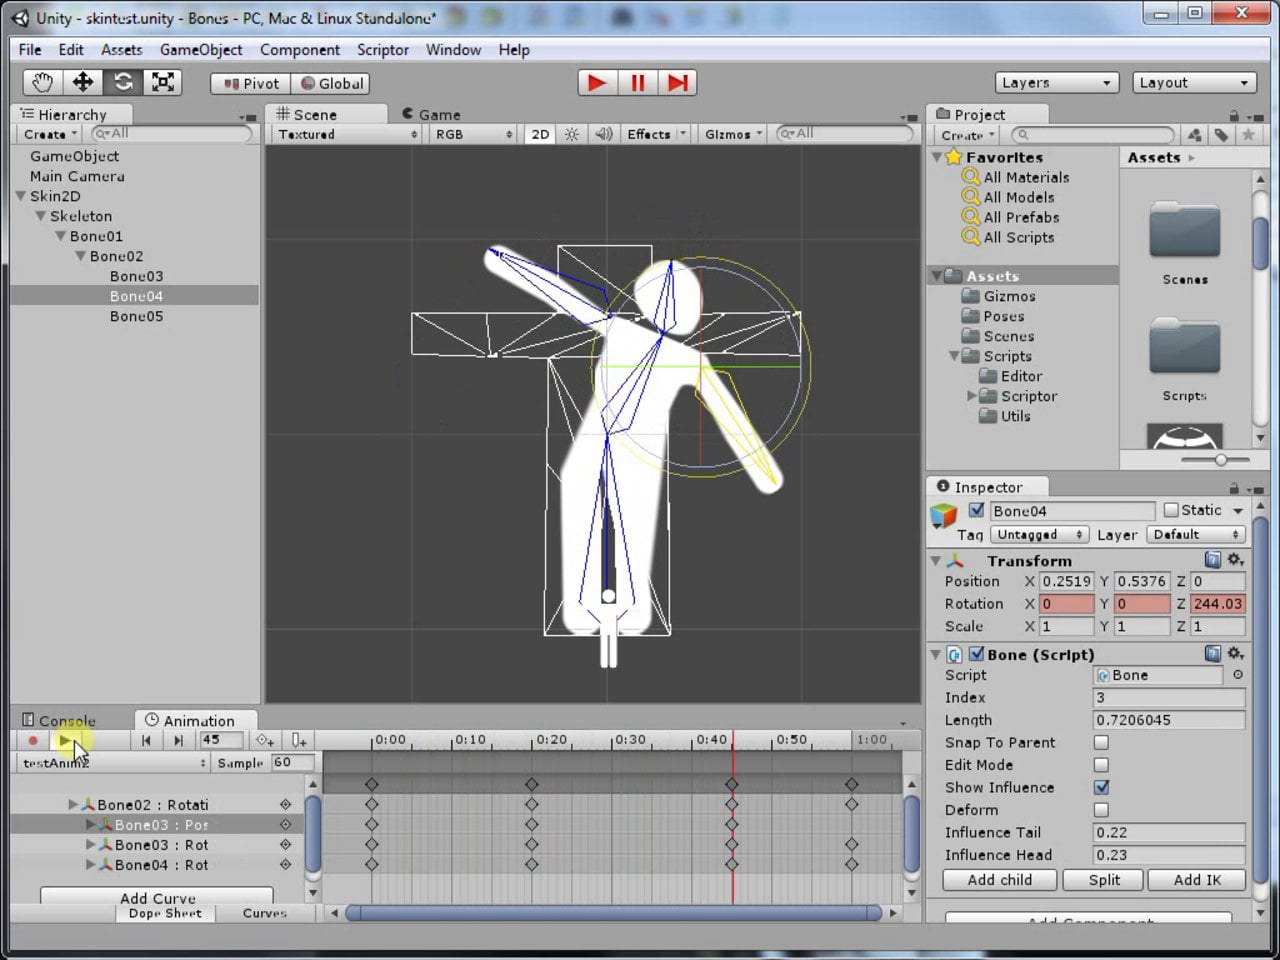
\includegraphics[width=\textwidth]{images/bones.jpg}
  }
  \caption{Pantalla de animaci�n de \emph{Unity 3D}.\\Fuente:\protect\url{https://i.vimeocdn.com/video/459915521_1280x960.jpg}}
  \label{fig:unityBones}
\end{figure}

Grabar una macro de animaci�n es muy simple: solo hay que situarse sobre el GameObject que queremos animar y darle a ''a�adir nueva animaci�n''. Nos saldr� una ventana como la de la figura \ref{fig:unityBones}. En el cronograma marcamos el 0 como el estado actual del objeto. Pulsamos grabar. Deformamos el GameObject (rotaciones, escalados,etc) y vamos a�adiendo marcas de tiempo por cada deformaci�n hasta un estado final. Autom�ticamente el sistema se encarga de crear la animaci�n haciendo que las deformaciones sean progresivas.

Ya solo nos queda definir cu�ndo lanzar la animaci�n y eso se hace gracias al sistema de m�quina de estados que nos permite definir \emph{Unity 3D}. En �l simplemente vamos definiendo estados, partiendo de uno de inicio, y asignado condiciones para que ocurra el cambio de estado. Desde el c�digo vamos lanzado dichas condiciones que pueden ser de dos tipos: triggers (disparadores) o condiciones l�gicas.

\subsubsection{Recursos y componentes: Asset Store}
Una de las principales ventajas de \emph{Unity 3D} es la capacidad para aprovechar el trabajo de otros para poder usarlo en nuestro beneficio personal. Como ya he comentado, el uso de Prefabs permite reutilizar componentes ya creados anteriormente. Tambi�n se puede llevar a otro punto: existe una tienda virtual, llamada \emph{Asset Store} en la que la comunidad y empresas pueden regalar o vender sus Prefabs y componentes para que otros puedan usarlos. A estos Prefabs y componentes se les llama Assets y van desde terrenos y animaciones a modelos 3D. Adem�s, es la plataforma desde la que los desarrolladores de \emph{Unity 3D} comparten y distribuyen los Assets b�sicos a los que puede acceder cualquiera que use \emph{Unity 3D}.

\lsection{Requisitos}

Cualquier sistema de software responde a una necesidad. Dicha necesidad debe analizarse por partes de manera que sea m�s sencilla su implementaci�n. Divide y vencer�s. En este apartado se hace justamente eso, se divide el sistema en las funcionalidades y requisitos que debe tener. Hay que constatar que no todos los requisitos tienen el mismo nivel de prioridad y que en este TFG no todos han sido resueltos, ya que como se coment� anteriormente este proyecto est� desarrollado con la intenci�n de continuarse y de seguir evolucionando. Por ello se dividir� en requisitos funcionales fundamentales y no fundamentales, que ser�n pospuestos para una versi�n dos. Muchos de estos requisitos no funcionales derivan de una falta de tiempo para el desarrollo del sistema.

\subsection{Requisitos funcionales}
Los requisitos funcionales son todas aquellas funcionalidades o casos de ejecuci�n que el sistema debe ser capaz de realizar y cumplir.

\subsubsection{Fundamentales}

\paragraph{El sistema debe tener un dise�o modular para que se pueda modificar con sencillez.}
La modularidad debe ser fundamental en este sistema para que su evoluci�n sea propicia. Este es uno de los principales motivos por los que se ha elegido \emph{Unity 3D} como entorno de desarrollo. Este entorno nos permite, con sus Prefabs, definir objetos que implementan funcionalidades. En este caso, con Prefabs se implementa un navegador web, un sistema de informaci�n de fecha y hora constante, un sistema de men� y un sistema de eventos que generan una interfaz de uso con el usuario.

\paragraph{El sistema debe dar capacidad al usuario de interaccionar con los elementos del escenario que le rodea.}
El usuario ha de ser capaz de interaccionar con lo que le rodea dentro de la escena del mundo virtual. Para ello se han desarrollado los siguientes dos m�dulos.
\begin{itemize}




\item El primer m�dulo permite una interacci�n del usuario y los componentes propios gr�ficos del entorno virtual.
\item El segundo permite una emulaci�n de eventos de click de cara al sistema y de pulsaci�n de teclas de teclado, es decir, emula un click de rat�n f�sico y una pulsaci�n de tecla f�sica. En la secci�n \ref{sect:desarrolloSistema} se explicar�n los motivos.

\end{itemize}


\paragraph{El sistema debe dar al usuario en todo momento informaci�n de fecha y hora actuales.}
El sistema proporciona informaci�n de fecha y hora constante al presentar dichos valores como dos paneles flotantes a la vista del usuario.

\paragraph{El sistema debe disponer de una funcionalidad simple para apagarse.}
El sistema dispone de un men� en el que existe una opci�n para apagar el sistema. Hay que ser cautelosos en este punto, pues una persona con tetraplej�a puede apagar el sistema pero seguir� con las gafas puestas y con la vista tapada por una pantalla en negro. Debe haber presente un cuidador en este punto.

\paragraph{El sistema debe dar una funcionalidad para navegar por Internet.} 
El sistema dispone de un navegador con el que interaccionar basado en la tecnolog�a \emph{Chromium} \citep{article:Chromium} de la empresa \emph{Thunderbeast Games LLC} \citep{article:UWEBKIT} que ha sido modificado para adaptarlo al proyecto en cuesti�n.

\subsubsection{No fundamentales}

\paragraph{El sistema debe ser capaz de realizar un autoajuste en funci�n de la discapacidad del usuario.}
Este requisito se ha clasificado como no fundamental debido a que la complejidad que supone se escapa del �mbito del TFG. El coste de desarrollo de esta funcionalidad es demasiado elevado. Como se ha visto en la secci�n \ref{sect:discMotoras} existe un gran n�mero de casos a tener en cuenta. Como punto de partida de desarrollo de esta funcionalidad ser�a la implementaci�n de un sistema de adaptaci�n al movimiento del cuello del usuario en base a un algoritmo de aprendizaje. Muchos de estos puntos por s� solos podr�an ser objeto de estudio de un TFG.

\paragraph{El sistema debe permitir configurar el aspecto visual del escenario principal que rodea al usuario.}
Uno de los principales motivos por los que Steve Jobs tuvo �xito con su \emph{Macintosh} fue por la idea de a�adir una interfaz de usuario amigable y personalizable, alejando a los computadores de la t�pica terminal de fondo negro y letra verde. Esto demuestra que el �xito de la aceptaci�n del sistema por parte del usuario depende en parte del aspecto y las posibilidades de �ste de ser adaptado a los gustos del individuo.

\subsection{Requisitos no funcionales}
Los requisitos no funcionales responden a las necesidades del sistema que no influyen en una funcionalidad o en un caso de uso que debe cumplirse. Engloba caracter�sticas de tipo hardware, econ�micas o similares.

\subsubsection{Fundamentales}
\paragraph{El sistema debe ser capaz de ejecutar el mayor n�mero de dispositivos posible con fluidez.}
Para que se cumpla este requisito es necesario entender que es lo computacionalmente m�s costoso para el sistema. El mayor coste est� en el coste computacional de generar los gr�ficos. Por ello, el dise�o gr�fico se ha hecho con texturas sencillas y pocas animaciones. En fases de desarrollo se observ�, por ejemplo, que al poner muchos �rboles en el entorno 3D con animaciones de viento, la imagen en el \emph{Oculus Rift} iba a saltos.

\subsubsection{No fundamentales}
\paragraph{El sistema debe poder ejecutarse en m�viles}
Este requisito es deseable y gracias a \emph{Unity 3D} es relativamente sencillo de cumplir. El problema por el cual se ha delegado a un requisito no fundamental es debido a la complejidad de cumplir algunos de los requisitos funcionales que llevar�an el desarrollo de este trabajo al doble de tiempo. Se especificar�n estos motivos en la secci�n \ref{sect:desarrolloSistema}.

\lsection{Dise�o del sistema}
El dise�o de este sistema es algo complejo dado que est� muy influenciado por los propios patrones que fuerza \emph{Unity 3D} a seguir. Primero se explicar� la estructura en la que se ha dividido el c�digo en funci�n de las funcionalidades de cada nivel de la jerarqu�a. A continuaci�n se explicar�n los patrones \emph{Fa�ade}, \emph{Modelo-Vista-Controlador} y \emph{Composite} que son el patrones base que se usan.

\subsection{Estructura del c�digo}
En \emph{Unity 3D}, todo el c�digo, Prefabs o similar est�n en la carpeta denominada \emph{Assets}. Dentro de esta carpeta se encuentran los siguientes directorios:

\subsubsection{Cardboard}
En este directorio est� el SDK b�sico para la generaci�n de una versi�n destinada a dispositivos m�viles. Incluye scripts de correcci�n de distorsi�n para las im�genes estereosc�picas as� como un Prefab. Adem�s da una herramienta de debug que permite hacer pruebas en etapa de desarrollo sin tener a mano unas \emph{Google Cardboard}.

\subsubsection{Scenes} 
Aqu� se encuentra la escena de \emph{Unity 3D} donde se desarrolla toda la acci�n. Se recuerda que es en las escenas donde se posicionan los \emph{GameObjects} en los que se basa el sistema.

\subsubsection{System} 
\label{subsection:System}
En esta carpeta est�n las implementaciones que se han realizado en este TFG. Est�n las animaciones desarrolladas, los fuentes sobre los que se ha basado este TFG y las implementaciones creadas a partir de estos. 

\begin{itemize}
\item \textbf{Animations.} En este directorio se almacenan las animaciones creadas para este TFG. Existen en este momento dos: la primera corresponde a la animaci�n de la mirilla para dar un feedback al usuario cuando se vaya a ejecutar un evento de click y la segunda es la animaci�n destinada al despliegue del men� del sistema.

\item \textbf{PeterKoch.} En este directorio se almacena el software obtenido de \citep{article:Gaze} que se usa para implementar un sistema Gaze Input, el necesario para la interacci�n con los objetos tridimensionales del sistema. Se basa en un \emph{RayCaster}, que no es m�s que un vector que sale perpendicular a la c�mara, cuya funci�n es lanzar y emitir un evento que ser� registrado por el sistema. Es lo que se usa, por ejemplo, en un videojuego de disparos para que el sistema sepa a qu� punto se esta apuntando.

\item \textbf{Prefab.} En este directorio se almacenan aquellos Prefabs que est�n creados para a�adir de manera sencilla funcionalidades al sistema. Existe un Prefab que incluye la c�mara del sistema con la fecha, la hora del sistema y la mirilla con la que apuntar. De este Prefab existen dos versiones, una para Pc's y otra para m�viles.

\item \textbf{Scripts.} En este directorio se almacenan aquellos scripts para el desarrollo de las funcionalidades del juego, por ejemplo, el script que toma la fecha y hora del sistema y la plasma en vistas.

\end{itemize}

Existen m�s directorios que se omiten por ser irrelevantes. En dichos directorios hay componentes como el cielo que se presenta en el juego o ejemplos de uso de los componentes.

\lsection{Desarrollo del sistema}
\label{sect:desarrolloSistema}

Para el desarrollo del sistema se ha usado el patr�n de dise�o \emph{Fa�ade}, dado que permite enmascarar el uso de uno o varios sistemas complejos tras una interfaz simple y constante \citep{article:UML} permitiendo as� que se puedan cambiar de manera simple dichos sistemas complejos sin que se vea afectado el sistema global. Este patr�n se usa en el desarrollo del sistema de emulaci�n de eventos de click y de pulsaci�n de teclas del teclado. En el anexo \ref{Anexo:codigo} se puede observar el c�digo en el que se implementa este desarrollo.

Existe otro tipo de eventos, que son eventos de colisi�n del \emph{RayCaster} (explicado en la secci�n \ref{subsection:System}) con objetos, que son manejados por el propio sistema de \emph{Unity 3D} y que por tanto escapan a la posibilidad de dise�o siendo �sta heredada del motor de gesti�n propia de \emph{Unity 3D}. 

Los patrones que utiliza \emph{Unity 3D} que m�s se pueden percibir y que son los que m�s trata el usuario son los siguientes:
\begin{itemize}
\item \textbf{Composite} Este patr�n se caracteriza por su facilidad para implementar herramientas complejas a partir de elementos m�s sencillos. Suele estar presente en aquellos dise�os de interfaces gr�ficas. En caso de \emph{Unity 3D} no es distinto. Aunque este patr�n de dise�o no se haya usado en el c�digo de manera estricta, s� ha sido aplicado en el dise�o del men�, por ejemplo. El men� se compone de un canvas (panel sobre el que dibujar) al que se le a�aden botones \citep{article:UMLMVC}.

\item \textbf{Modelo-Vista-Controlador (MVC)} Este patr�n se basa en el concepto de la modularidad. La idea es separar la representaci�n f�sica de un componente, de su representaci�n conceptual y de su implementaci�n final. Es el modelo b�sico de \emph{Unity 3D} dado que es como se enfoca a usar los GameObject. Un dise�o bajo este patr�n se corresponde de tres partes. La primera es el \emph{Modelo}. El \emph{Modelo} corresponde con la estructura de los datos a representar. La segunda parte corresponde con la \emph{Vista}. La \emph{Vista} es la representaci�n de dicho modelo. Por �ltimo est� el \emph{Controlador} que es el puente de uni�n entre ambos. En \emph{Unity 3D} el GameObject es la vista del elemento que percibe el usuario. Por detr�s est�n los scripts desarrollados que extienden de \emph{Monobehaviour}. Es decir, la clase \emph{Monobehaviour} es el modelo, el GameObject de la escena la vista y el software que invoca las funciones heredadas de la clase \emph{Monobehaviour} es el controlador \citep{article:UMLComposite}.

\end{itemize}

Estos patrones son los que m�s afectan al usuario a la hora de realizar una funcionalidad en \emph{Unity 3D} pero no quiere decir que sean los �nicos. \emph{Unity 3D} es un sistema muy complejo que en su fuero interno aparecen m�s patrones como \emph{Observer}, \emph{Coroutines}, \emph{Singleton},etc.

\lsection{Diagrama de clases}

En las figuras \ref{fig:diagClases2} y \ref{fig:diagClases} se pueden observar los diagramas de clases que corresponden al dise�o de este trabajo. 

En la figura \ref{fig:diagClases2} se aprecia las vistas del dise�o, seg�n MVC. Las clases que descienden de \emph{GameObject} son los objetos tridimensionales de la escena. Est�n compuestas por otros componentes que tambi�n descienden de la clase \emph{GameObject} y que se omiten por que no aportan valor (botones, entradas de texto, etc). Un ejemplo de la fusi�n de los patrones \emph{Composite} y \emph{MVC}.

\begin{figure} [h!]
\centering	
	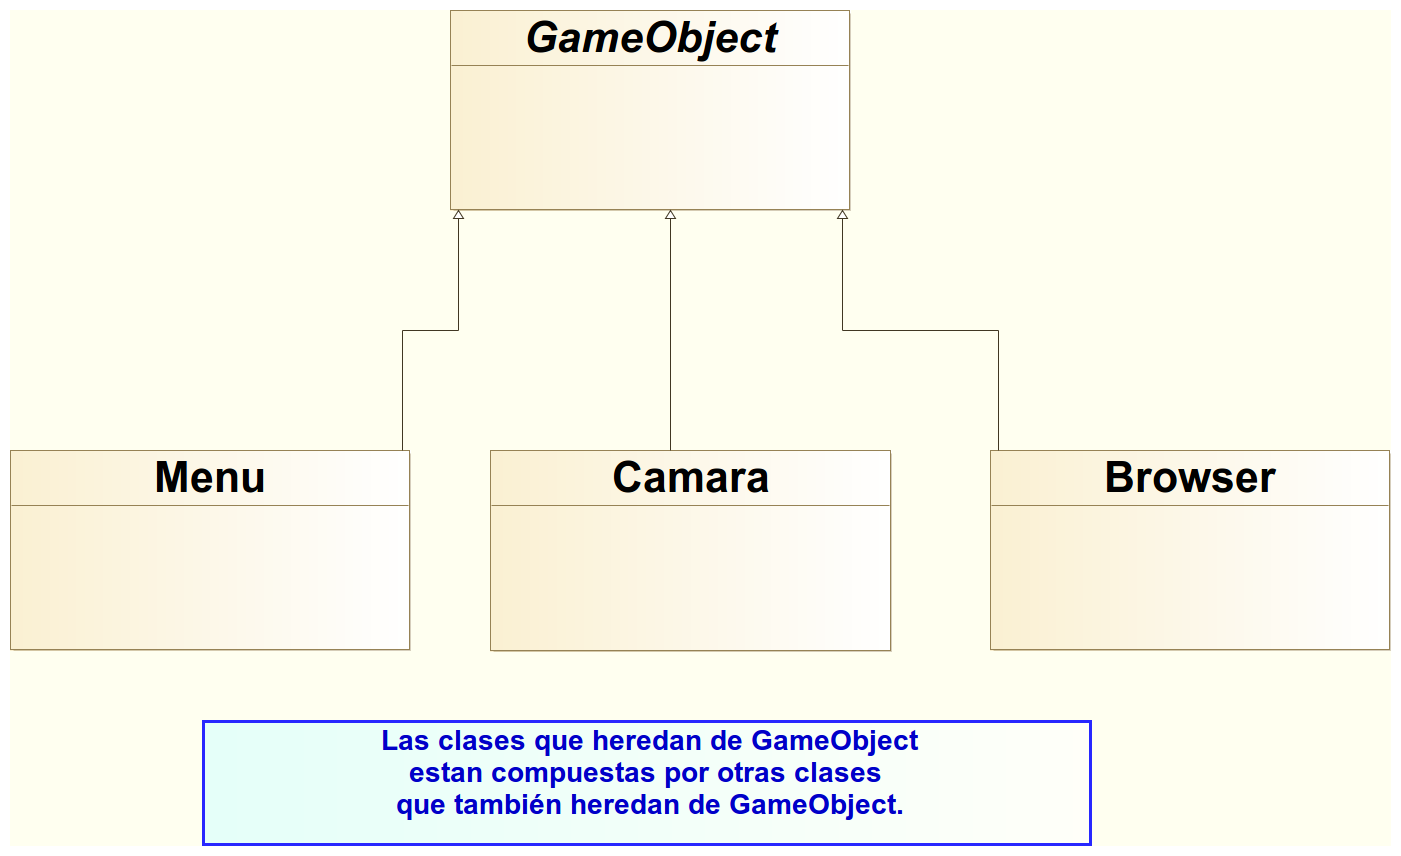
\includegraphics[width=\textwidth]{images/diagramaClases2.png} 
  \caption{Diagrama de clases de la aplicaci�n. Muestra las Vistas del patr�n MVC}
  \label{fig:diagClases2}
\end{figure}

En la figura \ref{fig:diagClases} se observa el diagrama de clases orientado a los controladores, seg�n MVC. A continuaci�n se a�ade una breve descripci�n de las clases mas relevantes:

\begin{itemize}
	\item Las clases que descienden de \emph{Monobehaivour} son independientes porque es el propio sistema el que ejecuta el m�todo \emph{OnUpdate} una vez por frame. 
	\item La clase \emph{InfoPanelController} se encarga de mostrar la hora y la fecha.
	\item La clase \emph{MenuTrigger} se encarga de controlar que aparezca o desaparezca el men� y de las opciones de �ste.
	\item La clase \emph{Quit} se encarga de cerrar la aplicaci�n. La clase \emph{WebTexture} se encarga de controlar el navegador de Internet. 
	\item Las clase \emph{GazeInputModule} es la que se encarga de la interacci�n con los GameObject del sistema. Adem�s maneja la funcionalidad para activar la animaci�n de la mirilla. Implementa el patr�n \emph{Fa�ade} al usar los m�dulos que permiten emular el evento f�sico de click y pulsaci�n de teclado. Se decidi� el uso del patr�n \emph{Fa�ade} debido a la intenci�n de, en un futuro, sacar una versi�n para dispositivos m�viles. Gracias a este patr�n, simplemente cambiando las clases \emph{MouseOperator} y \emph{KeyboardOperator} por dos clases espec�ficas para la plataforma m�vil (una que reproduzca un evento t�ctil en la pantalla y otra que escriba en el buffer de texto del sistema) se consigue adaptar el sistema a dispositivos m�viles.
\end{itemize}

%%%%%%%%%%%%%%%%%%%%%%%%%%%%%%%%%%%%%%%%%%%%%%%%%%%%% DIAGRAMA DE CLASES%%%%%%%%%%%%%%%%%%%%%%%%%%%%%%%%%%%%%%%%%%%%%%%%%%%%%%%%%%%%%%%%
\begin{landscape}
\begin{figure}  
\centering	
	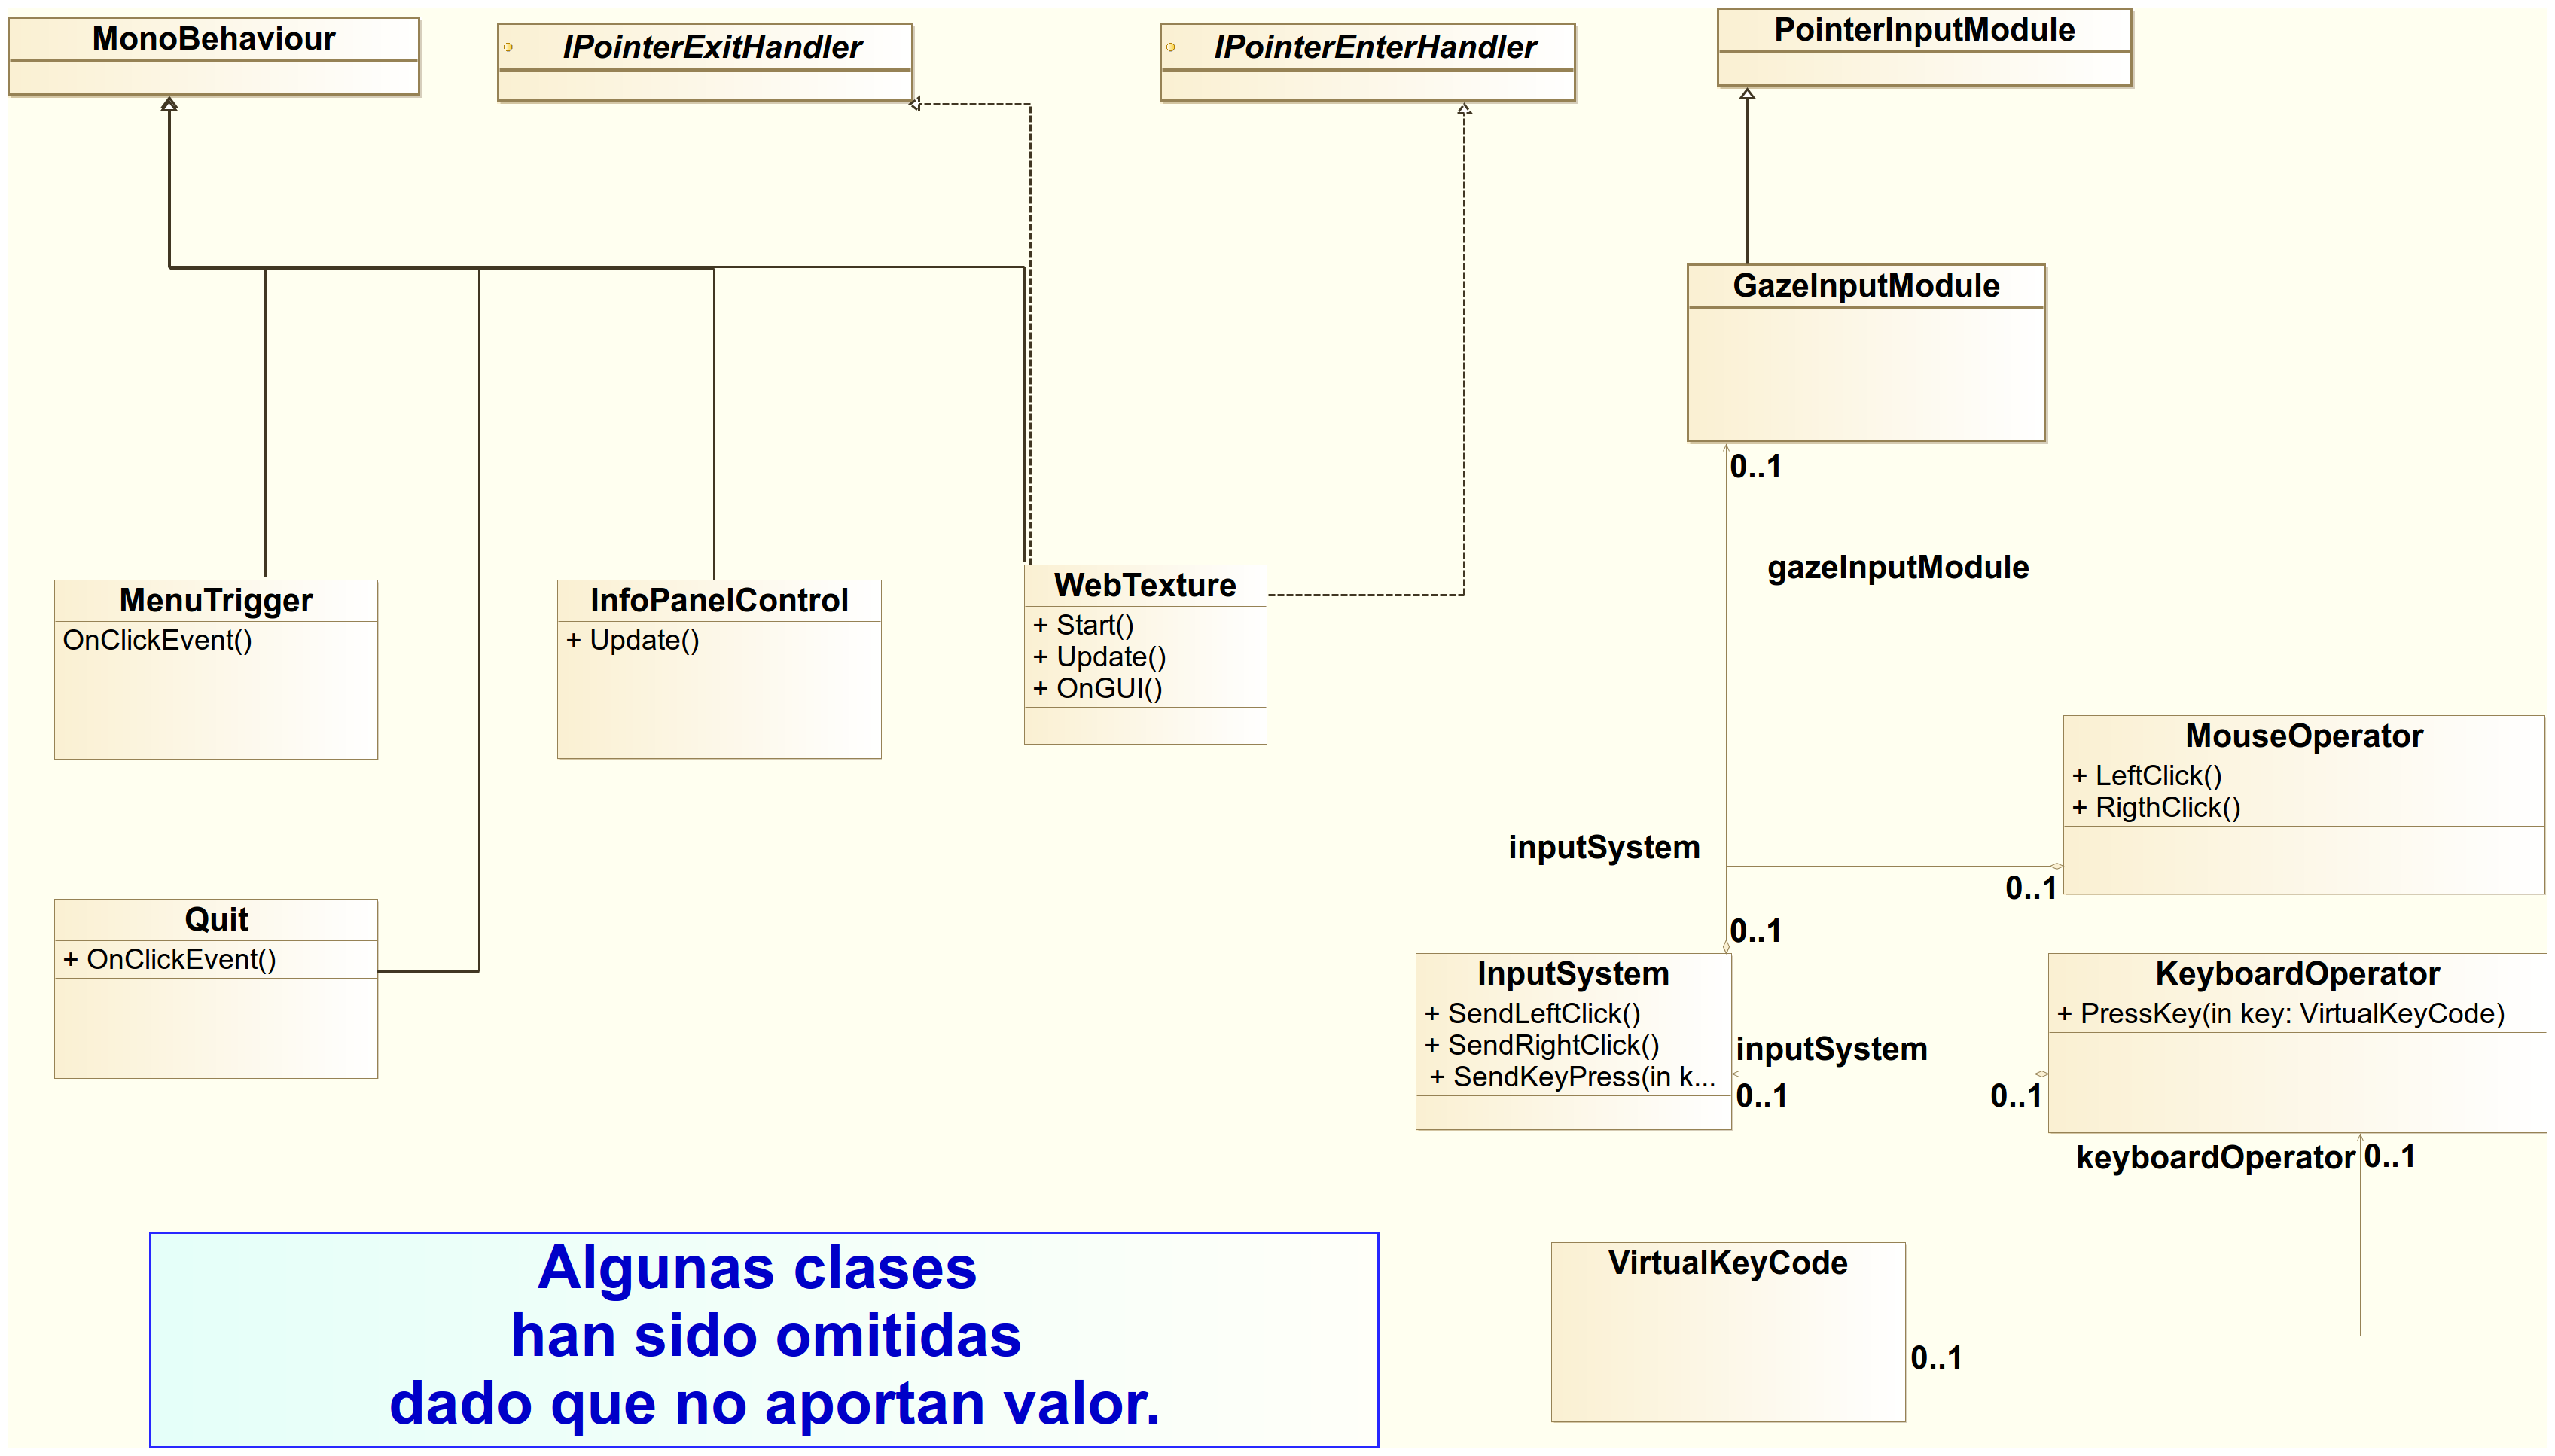
\includegraphics[height=0.8\textwidth]{images/diagramaClases.png} 
  \caption{Diagrama de clases de la aplicaci�n. Muestra los Controladores del patr�n MVC}
  \label{fig:diagClases}
\end{figure}
\end{landscape}
%%%%%%%%%%%%%%%%%%%%%%%%%%%%%%%%%%%%%%%%%%%%%%%%%%%%% DIAGRAMA DE CLASES%%%%%%%%%%%%%%%%%%%%%%%%%%%%%%%%%%%%%%%%%%%%%%%%%%%%%%%%%%%%%%%%

\lsection{Casos de uso}

A continuaci�n se expondr�n distintos casos de uso de la aplicaci�n que han servido como referencia de dise�o e implementaci�n de este trabajo. En dichos casos de uso se pueden observar dos actores: El actor \emph{Usuario}, es una persona en situaci�n de discapacidad que no puede ponerse por si solo los cascos de VR. Por ello aparece el segundo actor que es un cuidador. 

El primero de los casos es un caso de uso simple: el usuario debe ser capaz de interaccionar con un objeto del mundo virtual. Para ello se dise�a un caso de uso en el que el usuario tiene que abrir un men� desplegable y a posterior seleccionar la opci�n \emph{Salir} (figura \ref{fig:caso1}).

\begin{figure}[H]
\centering	
	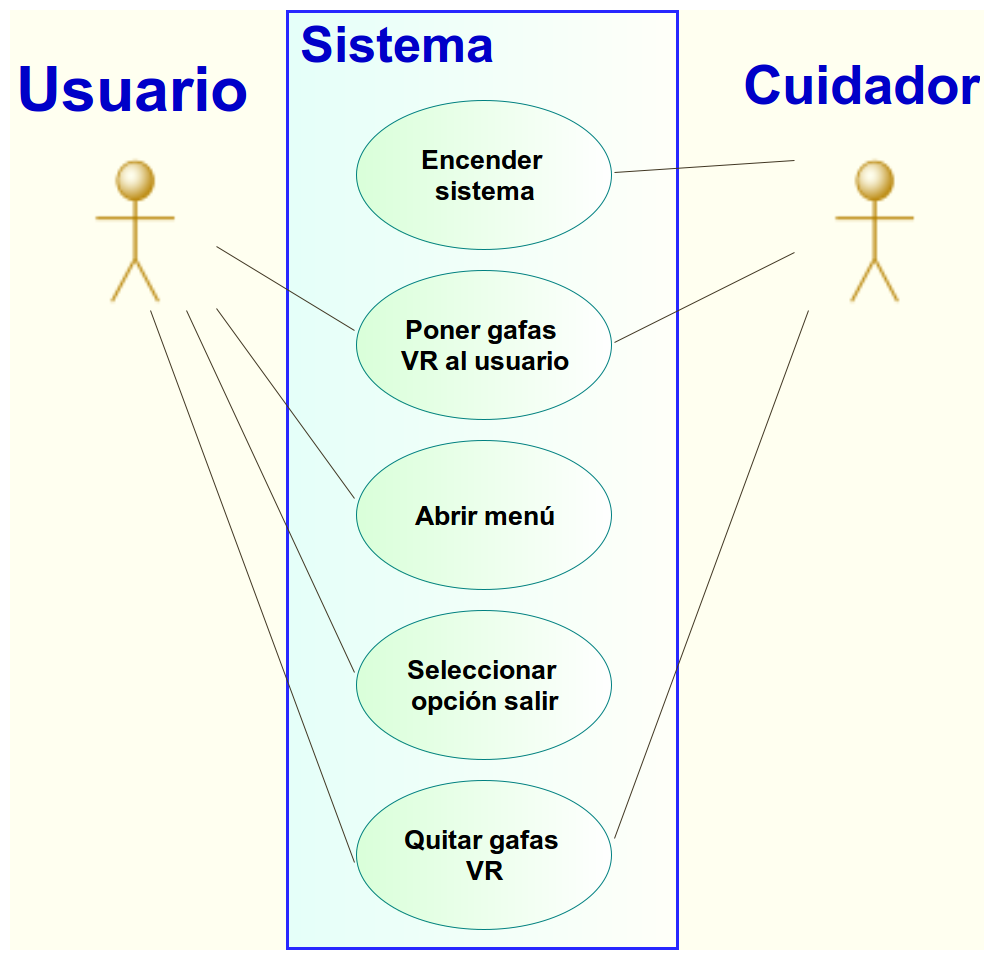
\includegraphics[width=\textwidth]{images/caso1.png} 
  \caption{Diagrama de caso de uso 1}
  \label{fig:caso1}
\end{figure}

El segundo caso de uso es en el que se representa la apertura del navegador y el cierre del mismo. El usuario debe abrir el men� desplegable, seleccionar la opci�n \emph{Open Browser} y esperar a que este se abra. A continuaci�n debe interaccionar con el mismo bot�n del men� para cerrar dicho navegador (figura \ref{fig:caso2}).

\begin{figure}[H] 
\centering	
	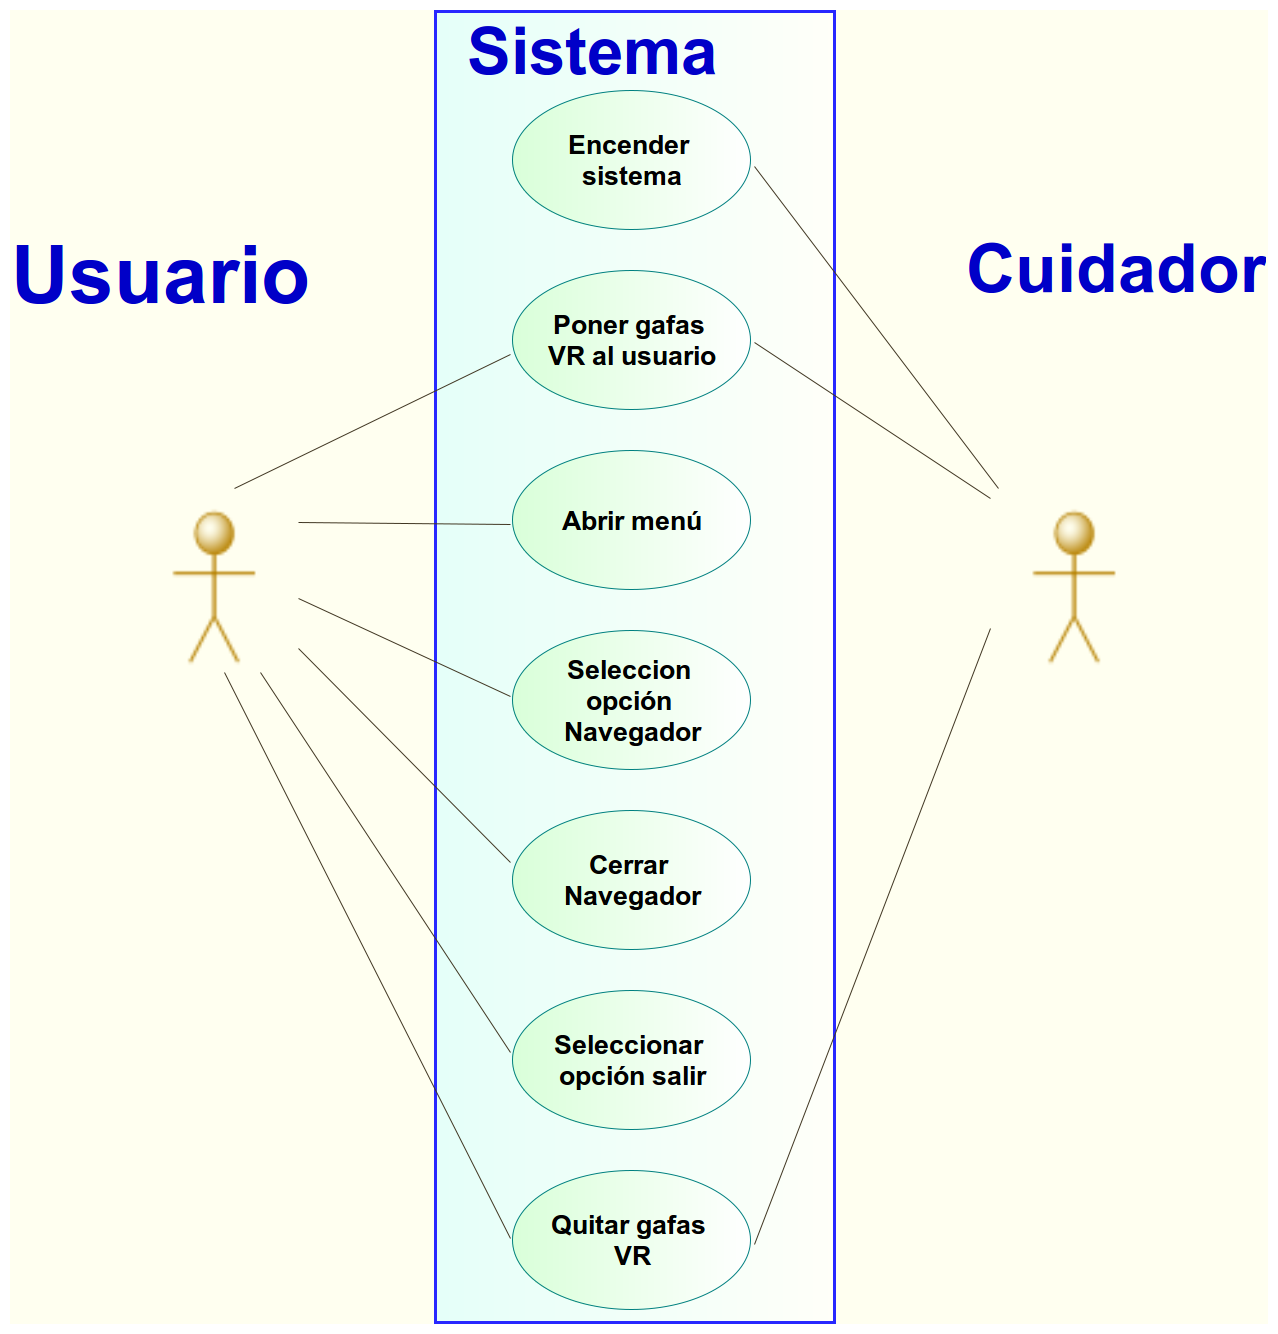
\includegraphics[width=\textwidth]{images/caso2.png} 
  \caption{Diagrama de caso de uso 2}
  \label{fig:caso2}
\end{figure}

El tercer caso de uso es en el que se representa la apertura del navegador y la navegaci�n por Internet. Para ello el usuario debe abrir el navegador, seleccionar el campo donde escribir la URL, interaccionar con el teclado para escribir la url \emph{www.youtube.es}, darle al bot�n \emph{Go} para cargar la p�gina, seleccionar un v�deo a reproducir y despu�s cerrar el navegador y el sistema (figura \ref{fig:caso3}).

\begin{figure}[H] 
\centering	
	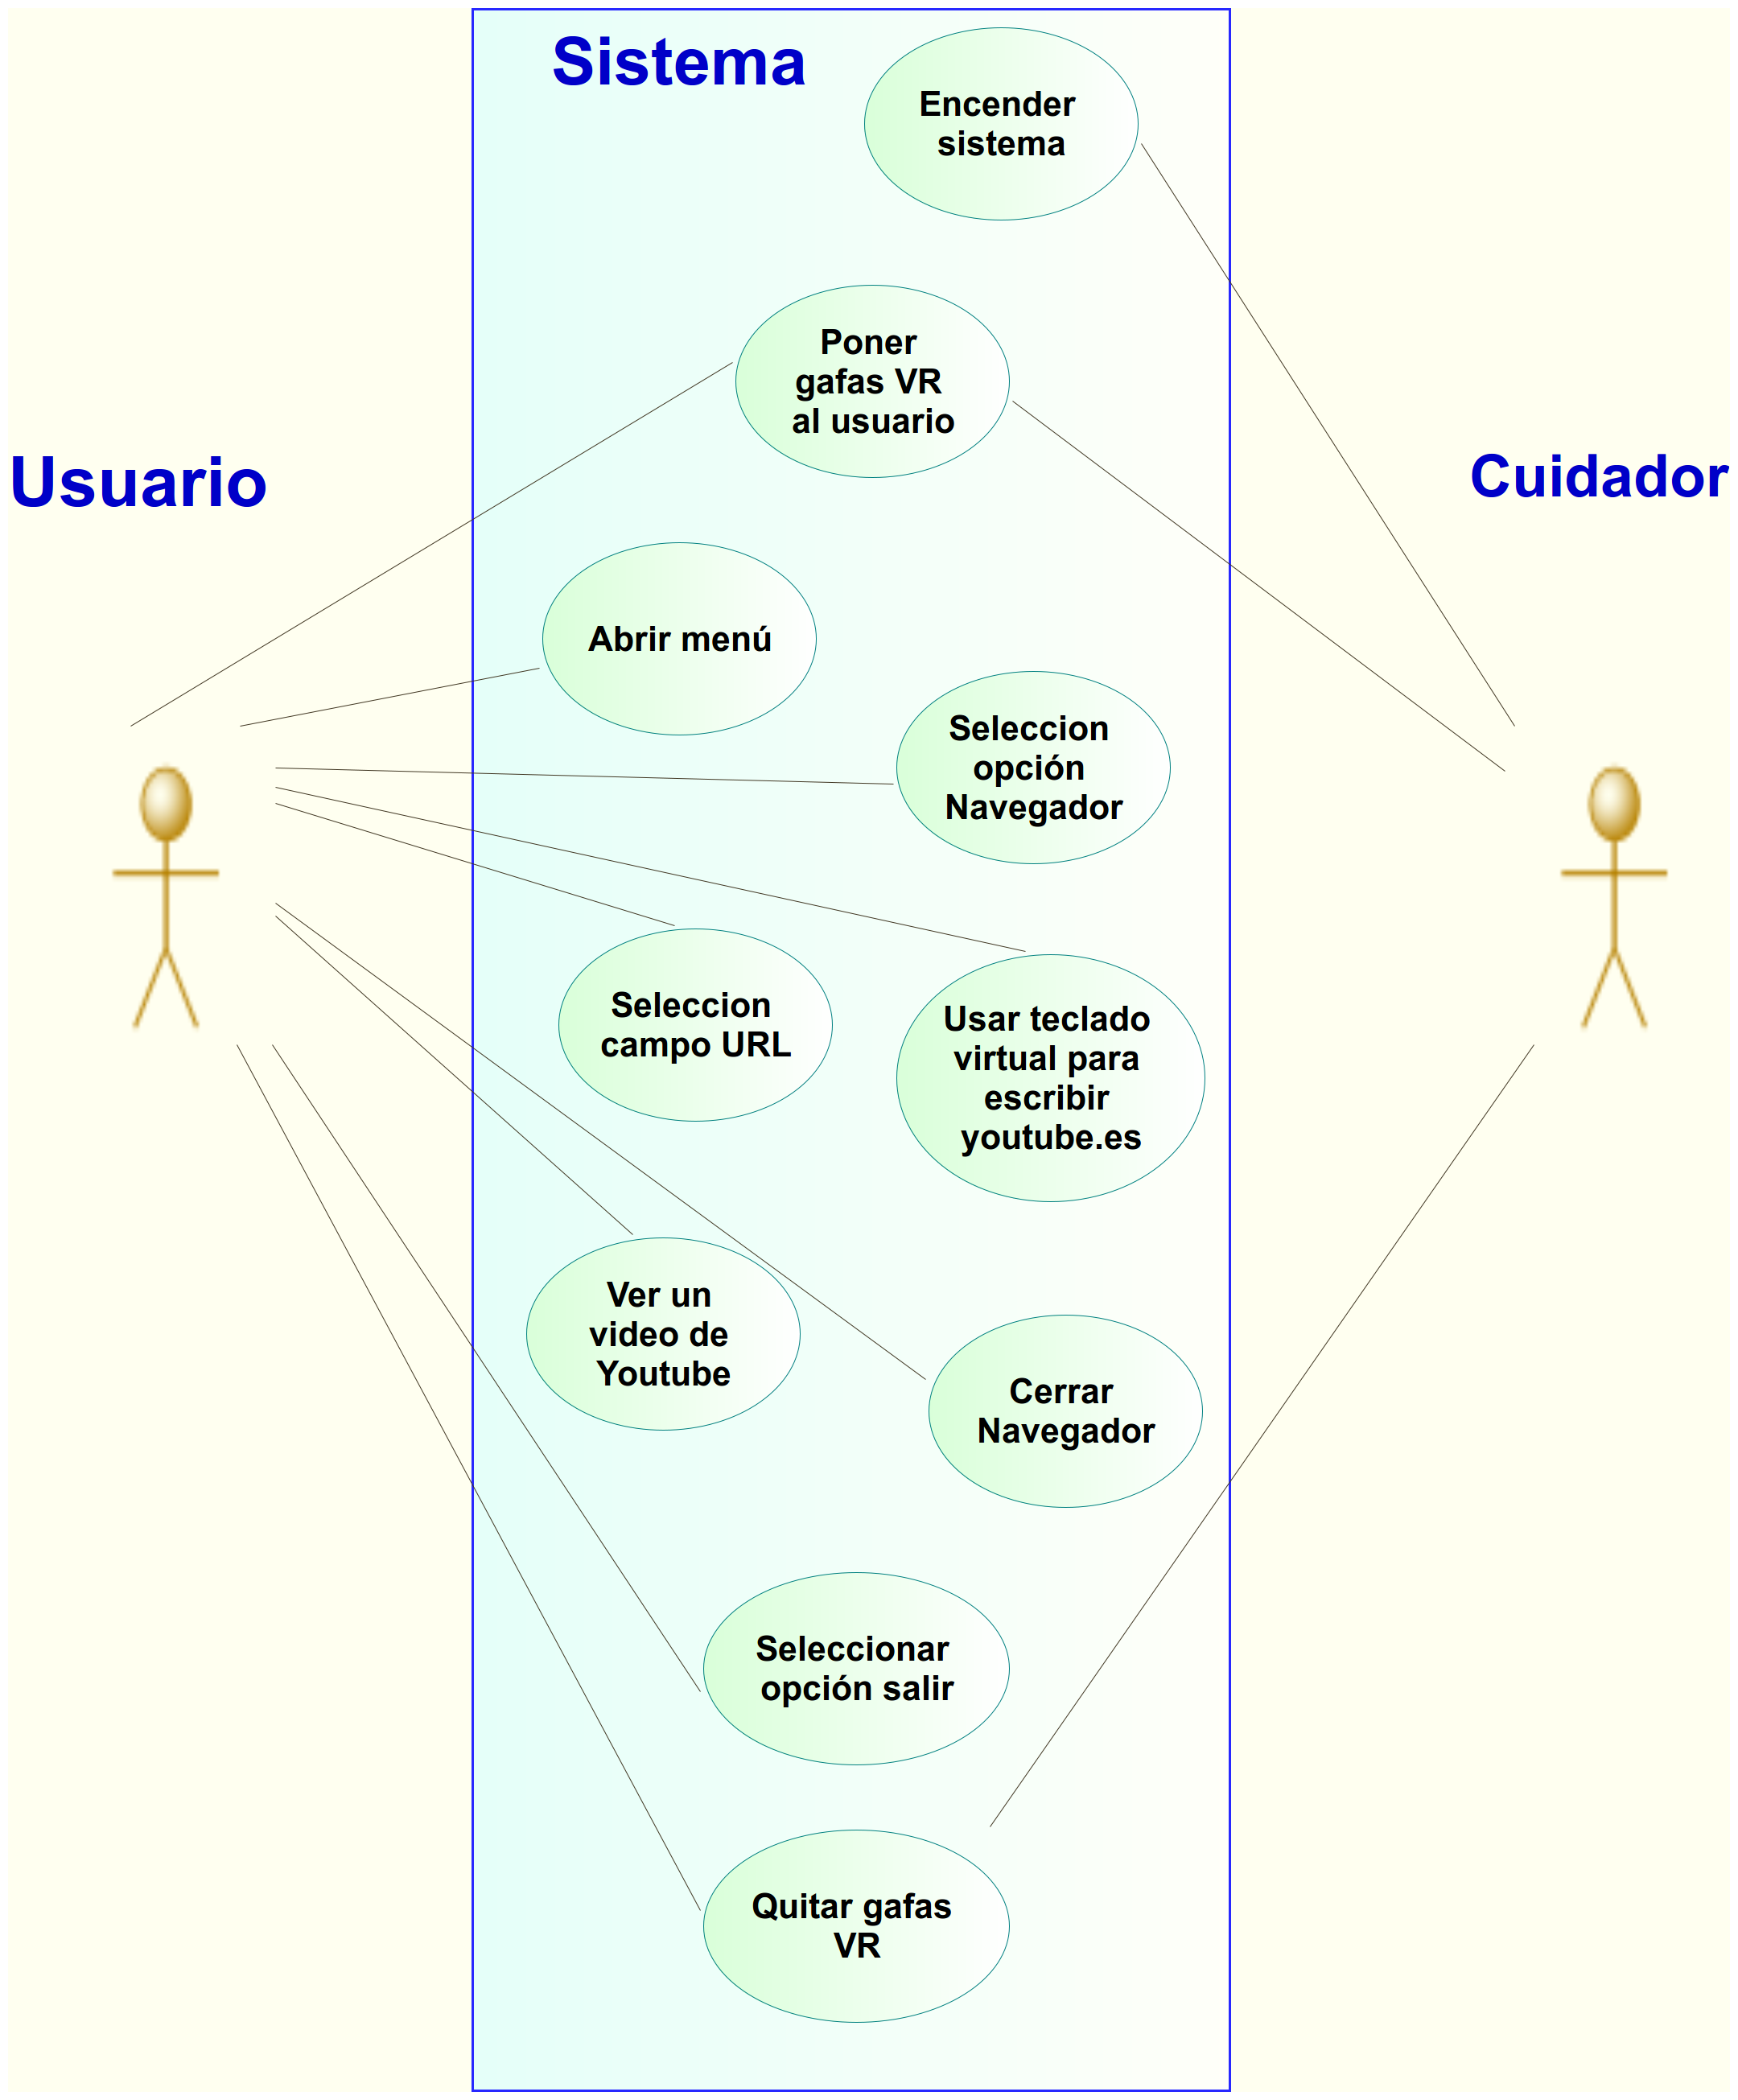
\includegraphics[width=\textwidth]{images/caso3.png} 
  \caption{Diagrama de caso de uso 3}
  \label{fig:caso3}
\end{figure}

En el anexo \ref{Anexo:casos} se encuentra una colecci�n de figuras del sistema que representan cada caso de uso. Dicho anexo est� dividido en secciones que corresponden a cada caso descrito.
\newpage

\lsection{Problemas encontrados y soluciones}
\label{sec:problemas}
En el desarrollo de este TFG surgi� un contratiempo que tuvo una gran repercusi�n en el proyecto. El problema era que la funcionalidad para implementar un navegador web no estaba soportada por \emph{Unity 3D}, lo que oblig� a buscar un software de terceros llamado \emph{uWebKit}, pues el desarrollo de un navegador est� fuera del �mbito de este TFG dado que su tiempo estimado de desarrollo es demasiado alto. La consecuencia del uso de este software fue tener que dejar de lado el desarrollo para dispositivos m�viles al no dar este software de terceros soporte a estas plataformas. Dicho software es de pago, siendo el coste de su licencia de unos 150\EUR. Afortunadamente, tras hablar con la empresa responsable por correo electr�nico y contarles las intenciones de este TFG y su finalidad acad�mica, decidieron proporcionar una licencia de desarrollo gratis \citep{article:UWEBKIT}. 

Tras esto, hubo que adaptar dicho software a las necesidades de este TFG pues no estaba destinado al uso de un m�todo de entrada como el usado en este trabajo. EL m�todo de entrada esperado para este software era un rat�n y un teclado. Por este motivo fue necesario desarrollar un m�dulo capaz de emular eventos de click en el sistema y otro m�dulo capaz de emular el evento que produce una pulsaci�n de una tecla del teclado. Para ello se usaron dos \emph{DLL} (una teclado, otra rat�n) que invocan llamadas al sistema para emular estas funcionalidades. 

El software de terceros utilizado \citep{article:UWEBKIT} usa la posici�n del rat�n de la siguiente manera: obtiene de \emph{Unity 3D} la posici�n del rat�n respecto a la escena y la adapta al sistema de referencia de la web. Por eso una vez resuelto el contratiempo de la emulaci�n de clicks hubo que enfrentarse al problema de transformar la posici�n de la mirilla a la posici�n del rat�n. Esto se consigui� gracias a los \emph{RayCaster} de \emph{Unity 3D} que b�sicamente proporcionaban informaci�n sobre las coordenadas a donde se apunta respecto a la escena. Solo fue necesario modificar que en lugar de obtener la posici�n inicial del rat�n, la obtuviera de este \emph{RayCaster}.

Antes de desarrollar la funcionalidad con este software se indag� en otras opciones de software libre como \emph{Awesomium} \citep{article:Awesomium}. Aunque existe un apartado de esta herramienta destinado a \emph{Unity 3D}, est� para una versi�n obsoleta (versi�n 3.4f) con lo que no se puede usar en la �ltima versi�n de \emph{Unity 3D} (5.2.1f) que es con la que se ha desarrollado este trabajo. La posibilidad de bajar de versi�n qued� descartada pues tanto el SDK de \emph{Google Cardboard} como el de \emph{Oculus Rift} no daban soporte a tales versiones de \emph{Unity 3D}.

Se exploraron otras opciones como el proyecto \emph{Chromium} \citep{article:Chromium} pero no se pod�a incluir de manera r�pida a \emph{Unity 3D} y en concreto a \emph{C\#}.

Para versiones m�viles existen alternativas adecuadas. Android ofrece un webViewer de manera nativa y en iOS est� implementado \emph{Safari} para uso de los desarrolladores con lo que no es dif�cil implementar estas funcionalidades en dichas plataformas. No se ha implementado debido a la falta de tiempo.

\chapter{Experimentos Realizados y Resultados}
\label{chap:experimentos}

En este apartado se explicar\'an los dos experimentos realizados y su resultado. El primero es un estudio simple sobre los efectos del uso de gafas de realidad virtual y el segundo es un estudio de comodidad y usabilidad del usuario final.

\lsection{Estudio de efectos de las gafas de realidad virtual}
\label{sect:rv_sickness}

El objetivo de este estudio es entender c\'omo afecta el uso de un HDM en las personas que lo van a usar. Existen multitud de estudios que demuestran que el uso de la realidad virtual puede provocar mareos o distorsi\'on de la realidad \citep{article:VRSickness}. En este experimento se ha escogido un conjunto de personas sin ning\'un problema motor. La idea es proporcionar al usuario un est\'imulo dentro de un mundo virtual con la intenci\'on de marear y provocar una distorsi\'on de la realidad.

Para esta prueba se ha utilizado un videojuego de control de un helic\'optero en un PC. El escenario en el que se sit\'ua el helic\'optero es una isla con un portaaviones y una plataforma de aterrizaje en el agua. Adem\'as, en el centro de la isla, pero a una considerable altura, hay un globo con cajas colgando y un misil dando vueltas alrededor del globo. Este espacio virtual no ha sido creado por mi sino que es una demo destinada al uso de \emph{Oculus Rift}. Su nombre es \emph{Heli-Heli} \citep{article:HeliHeli}.

Para este peque\~no estudio se ha utilizado las \emph{Oculus Rift DK2} como dispositivo HMD. Para controlar el helic\'optero se usa un joystick de la casa \emph{Thrusmaster}. Se utilizan tambi\'en unos cascos de audio para obtener una sensaci\'on mayor de inmersi\'on.

\subsection{Metodolog\'ia}
La metodolog\'ia de este experimento es bastante sencilla: primero se ajustan las \emph{Oculus Rift} de manera personalizada creando un nuevo perfil por usuario. Adem\'as, se tiene en cuenta si el usuario tiene alg\'un tipo de problema visual para seleccionar las lentes de tipo A o B, siendo las de tipo B para personas con defectos visuales. Se toma nota del tipo de defecto visual que tiene el usuario en caso de tenerlo y de si suele jugar habitualmente a videojuegos (denotado como si es \emph{Gamer}). Se le ponen las \emph{Oculus Rift} al usuario y se le explica en qu\'e consistir\'a el experimento. Por \'ultimo se colocan unos cascos de audio para obtener una mayor sensaci\'on de inmersi\'on en el juego.

A continuaci\'on se realiza la prueba: se deja al usuario entre cinco y diez minutos de vuelo libre para que se habit\'ue al entorno virtual. El tiempo var\'ia en funci\'on de la pericia del usuario. A continuaci\'on, el evaluador toma los controles del helic\'optero pudiendo ver el mundo virtual en el monitor del usuario sin tener que quitarle las gafas. El evaluador empezar\'a a realizar movimientos bruscos con el helic\'optero hasta provocar que este se descontrole y se estrelle en el suelo. Esta parte no dura m\'as de tres minutos. R\'apidamente, tras estrellar el helic\'optero, se le quita al usuario las gafas y los cascos de audio. En la URL del sistema ( \url{https://www.dropbox.com/sh/8t9zp9l3xyq49dt/AAAY5N9I96hA9H5zjL4hzKUpa?dl=0}) se encuentra un v\'ideo en el que se muestra un ejemplo de este experimento. 

Se le pregunta al usuario si ha sentido v\'ertigo, mareos y/o distorsi\'on de la realidad.

\subsection{Resultados}
Este experimento se realiz\'o a seis individuos que dieron los siguientes resultados:

\begin{table}[htb]
	\centering
    \scriptsize
	\begin{tabular}{|l|l|l|l|l|}
		\hline
		\multicolumn{5}{|c|}{Resultados} \\ \hline
		Tipo Lente & Gamer & V\'ertigo & Mareos & Distorsi\'on Realidad\\
		\hline
		B & S\'i & No & S\'i & No\\ \hline
		B & No & No & S\'i & S\'i\\ \hline
		A & No & No & No & S\'i\\ \hline
		A & S\'i & No & S\'i & No\\ \hline
		B & No & No & S\'i & S\'i\\ \hline
		A & S\'i & No & S\'i & No\\ \hline
	\end{tabular}
	\caption{Resultados de test de efectos de las \emph{Oculus Rift DK2}. La primera columna corresponde al tipo de lente. La segunda columna a la pregunta de si el usuario suele jugar a videojuegos. La tercera columna corresponde a la pregunta de si tras la prueba, el usuario ha sufrido v\'ertigo. La cuarta columna a si a sufrido mareos. La quinta columna representa la respuesta a la pregunta de si el usuario ha sufrido distorsi\'on de la realidad.}
	\label{tabla:test1}
\end{table}

\subsection{Conclusiones}

Tras observar los datos de la tabla \ref{tabla:test1}, aunque sean poco representativos dado el peque\~no tama\~no muestral, podemos sacar como conclusi\'on que los usuarios no tienen sensaci\'on de v\'ertigo dada la altura del helic\'optero virtual. Esto se puede explicar razonando que la sensaci\'on de inmersi\'on no es lo suficientemente alta. No tenemos realmente sensaci\'on de altura. Por otro lado, casi todos los usuarios se marearon debido a los r\'apidos movimientos del helic\'optero al dar tumbos.

Tambi\'en se observa que los usuarios que tienen tendencia a jugar habitualmente a videojuegos est\'an m\'as acostumbrados a escenarios 3D y no tienen tanta distorsi\'on de la realidad al hacer el cambio repentino del mundo tridimensional al real. Esto demuestra que este sistema tiene una etapa de entrenamiento y que la capacidad para usarlo durante m\'as tiempo va incrementando con su uso.


Estos resultados nos dan a entender que el uso prolongado de un sistema de VR es perjudicial. Si nos fijamos en la tabla \ref{tabla:test1} podemos observar como todos los usuarios menos uno sufri\'o de mareos. \emph{Oculus Rift} muestra al inicio de cualquier aplicaci\'on un mensaje de advertencia del uso prolongado de su sistema. En este trabajo esto es un punto muy importante a tener en cuenta pues una PSD no tiene la capacidad para quitarse por si solo las gafas. Debe estar bajo la supervisi\'on de un cuidador.

\lsection{Estudio de comodidad y usabilidad del sistema}
\label{sect:rv_sickness}

Por \'ultimo se ha realizado un test de usabilidad. Las herramientas de accesibilidad van muy por detr\'as del uso com\'un del PC por lo que cabe esperar que esta herramienta frente a un uso convencional del PC sea m\'as lenta. Para hacer esta comparativa se han seleccionado otra vez usuarios que no tienen ning\'un problema o trastorno de movimiento dado que realizar estas pruebas con personas en situaci\'on de discapacidad es demasiado dif\'icil debido la preparaci\'on necesaria, los permisos y los tramites burocr\'aticos´e.

Para esta prueba se utiliza el sistema desarrollado. Cuenta de un men\'u desplegable, al que se accede a trav\'es del sistema de interacci\'on con la mirada, con una opci\'on para abrir el navegador. Un ejemplo del despliegue y de la selecci\'on de la opci\'on para abrir el navegador se puede ver en el anexo \ref{Anexo:caso3}.
 
El escenario f\'isico de este sistema es un PC y las \emph{Oculus Rift DK2}.

\subsection{Metodolog\'ia}
La idea es contrastar el sistema frente al uso convencional de un PC. Para ello primero se temporiza el tiempo que tarda en realizar una tarea determinada con un sistema de entrada com\'un y al que est\'a acostumbrado, es decir, teclado y rat\'on. Luego se hace una medici\'on de lo que tarda el usuario con el sistema actual tras haberle explicado verbalmente, sin previo entrenamiento (SE), como utilizar el sistema. A continuaci\'on se le da entre tres y cinco minutos de uso libre con el sistema tras los cuales se realiza otra medici\'on de tiempo. La intenci\'on con estos minutos de uso libre es que el usuario se adapte al sistema y entrene con \'el (CE).

La tarea a realizar es la misma en los tres pasos y consiste en entrar al portal de \emph{Youtube} a trav\'es de la URL \emph{www.youtube.es}, en el buscador escribir la palabra \emph{eps} y seleccionar el primer video.

Para la primera parte se realiza dicha tarea con el navegador \emph{Mozilla Firefox} y el teclado f\'isico. La segunda y tercera parte se realiza con el software presentado para este TFG usando la opci\'on de navegador y el teclado implementado. Un ejemplo de esto puede verse en el anexo \ref{Anexo:caso3}. 

En la URL del sistema (URL!!!) se encuentra un v\'ideo en el que se muestra un ejemplo de este experimento.

\subsection{Resultados}

Este experimento se realiz\'o con diez individuos acostumbrados al uso de las TIC pero sin previa noci\'on del sistema presentado en este TFG. Se obtuvieron los siguientes resultados:

\begin{table}[H]
	\centering
    \scriptsize
	\begin{tabular}{|l|l|l|l|}
		\hline
		\multicolumn{4}{|c|}{Resultados} \\ \hline
		Tipo Lente & T.Firefox & T.Sistema (SE) & T.Sistema (CE)\\
		\hline
		B & $19.66$ & $146.26$ & $45.06$\\ \hline
		A & $15.03$ & $142.21$ & $60.26$\\ \hline
		A & $12.49$ & $116.02$ & $59.96$\\ \hline
		B & $13.57$ & $83.33$ & $93.16$\\ \hline
		A & $14.75$ & $134.09$ & $115.31$\\ \hline
		A & $20.39$ & $112.57$ & $111.44$\\ \hline
		B & $16.79$ & $97.07$ & $80.06$\\ \hline
		A & $13.60$ & $106.46$ & $83.22$\\ \hline
		A & $14.71$ & $56.29$ & $55.05$\\ \hline
		A & $16.54$ & $77.17$ & $71.36$\\ \hline
	\end{tabular}
	\caption{Resultados de test de comodidad y usabilidad. La primera columna corresponde al tipo de lente usada. La segunda columna corresponde al tiempo usando teclado, rat\'on y el navegador \emph{Mozilla Firefox}, la tercera columna corresponde a los tiempos usando el sistema de este trabajo sin entrenamiento, la cuarta columna corresponde a los tiempos del sistema desarrollado en este trabajo con entrenamiento de tres a cinco minutos. Resultados de tiempos en segundos. }
	\label{tabla:test2}
\end{table}

\begin{table}[H]
	\centering
    \scriptsize
	\begin{tabular}{|l|l|l|}
		\hline
		\multicolumn{3}{|c|}{Media de Resultados} \\ \hline
		T.Firefox & T.Sistema (SE) & T.Sistema (CE)\\
		\hline
		$15.75 \pm 2.61$ & $107.15 \pm 29.34$ & $77.49 \pm 23.72$\\ \hline
	\end{tabular}
	\caption{Medias y desviaci\'on est\'andar de los datos obtenidos en la tabla \ref{tabla:test2}. Resultados de tiempos en segundos. }
	\label{tabla:test3}
\end{table}
\subsection{Conclusiones}

Tras observar los datos de las mediciones mostradas en la tabla \ref{tabla:test2}, podemos sacar en claro que, como se esperaba, los tiempos entre el uso de un rat\'on y teclado son mucho menores que los del sistema desarrollado en este trabajo. Por otro lado tambi\'en se observa que con solo escasos tres minutos de aprendizaje los tiempos de uso se reducen bastante.

Queda claro que este sistema necesita de entrenamiento por parte del usuario. Aun as\'i permite la interacci\'on con las TIC en unos tiempos dentro de un marco aceptable. Estos tiempos podr\'ian disminuirse aun mas mejorando la algoritmia de determinados componentes as\'i como innovando nuevas formas de interacci\'on que no sean las descritas en este trabajo.

\chapter{Conclusiones, discusi�n y trabajo futuro}
\label{chap:conclusiones}

Tras hacer este trabajo se puede sacar como conclusi�n que el desarrollo de un sistema tan amplio esconde muchos problemas que surgen con el paso del tiempo y el desarrollo del mismo. Aun as� he podido sentar las bases y generar una herramienta �til y que ayude a las personas. Los dos experimentos realizados han demostrado que, aunque aun le queda mucho camino por recorrer a este sistema, actualmente puede ser utilizado con la esperanza de buenos resultados. El primer experimento a confirmado que hay que tener cuidado con los efectos secundarios de sistemas de VR. El segundo experimento ha confirmado que con este sistema se interacciona con las TIC de siete a cinco veces m�s lento en valor promedio respecto al uso de teclado y rat\'on. Aunque, teniendo en cuenta el sector de la sociedad para el que va dirigido y sus dificultades, es un rango aceptable aunque mejorable. La soluci�n al problema de acercar las TIC a las PSD es dif�cil pero no imposible y la tecnolog�a avanza sin cesar.

No ser�a posible realizar un trabajo como este sin la previa documentaci�n y estudio de los sistemas a utilizar. Se parte de la base del desconocimiento total de dichos sistemas, como por ejemplo \emph{Unity 3D}. Esta tarea de documentaci�n y aprendizaje ha sido muy costosa en tiempo y en esfuerzo, siendo imposible de realizar si no llegara a ser por cursos online y videotutoriales de Internet \citep{article:Tutellus}. Aun as�, el desarrollo de este sistema me ha permitido dar un paso adelante en mi formaci�n. Estos son los conocimientos adquiridos en desarrollo de este trabajo:

\begin{itemize}
	\item \textbf{Unity 3D}
	\item \textbf{C\#}
	\item \textbf{JavaScript en profundidad}
	\item \textbf{Teor�a del dise�o de videojuegos y espacios tridimensionales}
	\item \textbf{Nuevos patrones de dise�o (Fa�ade,Proxy,etc)}
	\item \textbf{Uso de sistemas de realidad virtual completa como Oculus Rift}
	\item \textbf{Latex}
\end{itemize}

He podido comprobar de primera mano c�mo una buena planificaci�n y un buen dise�o pueden llegar a ser fundamentales. Cuando inici� este TFG y decid� hacer un m�dulo para la c�mara de Android y otro para la c�mara de \emph{Oculus Rift} no sab�a que tendr�a que dejar a medias el desarrollo para Android debido al problema del navegador mencionado. Esto podr�a haberse vuelto un problema verdaderamente complicado si no llega a ser por el dise�o modular.

Por otro lado, he podido profundizar m�s en un tema que me interesa como es la realidad virtual y encauzar mi futuro hacia la investigaci�n. Quiero recalcar en la cantidad de investigaci�n y pruebas que he tenido que superar y realizar para terminar con el software que se describe en esta memoria.

Como coment� en la introducci�n de esta memoria, este trabajo tiene la f�rrea intenci�n de marcar las bases de una herramienta que ayude a las personas. Por este motivo, su desarrollo debe continuar tanto por mi parte como por la de la comunidad, o al menos eso espero. Teniendo en cuenta los problemas que me han surgido en el desarrollo, establezco a trav�s de este apartado los que yo creo que deber�an ser los pasos a seguir para el crecimiento y trabajo futuro de esta herramienta:

\begin{itemize}
\item \textbf{Algoritmo predictivo de movimiento en ciclo cerrado.} Las PSD sufren distintos tipos de impedimentos. Hay casos de par�lisis parcial de los movimientos cef�licos que produce que estos movimientos no sean fluidos. El desarrollo de un algoritmo de aprendizaje y adaptaci�n para cada caso aportar�a al sistema una funcionalidad que ayudar�a much�simo a este sector. 

\item \textbf{Desarrollar un navegador para m�viles.} Este problema fue una desilusi�n por mi parte, pues ten�a la intenci�n de poder sacar una versi�n para m�vil a la par que para ordenador. Lamentablemente, esta funcionalidad no est� integrada en \emph{Unity 3D} y el coste en tiempo que supone para su desarrollo es amplio. Herramientas como \emph{Awesomium} \citep{article:Awesomium} y \emph{Chromium} \citep{article:Chromium} pueden ser un buen punto de partida. La idea de generalizar este trabajo a un dispositivo m�vil a mi parecer es muy atractiva, dado que el coste del sistema completo (gafas vr + software) se reduce dr�sticamente.

\item \textbf{Desarrollar nuevos m�dulos como clientes de correo, editores de texto,etc} Esta herramienta proporciona una funcionalidad b�sica: navegar por Internet. Aun as� se podr�an desarrollar m�s m�dulos que proporcionen nuevas herramientas como un cliente de correo, un editor de textos o un sistema de archivos.

\item \textbf{Incluir nuevos sistemas de entrada.} Se puede incluir m�s hardware que permita a�adir m�s funcionalidades. Como se ha visto en la secci�n \ref{sec:RVYDisc}, existen muchos proyectos que ayudan a las personas con discapacidad. Se podr�a incluir un sistema de seguimiento de ojos (m�s conocido en ingl�s como \emph{Eye Tracking}) que permita ver a d�nde se est� dirigiendo la mirada y mover la c�mara acorde a ello. Tambi�n se pueden incluir sistemas con \emph{BCI} que permitan detectar determinados tipos de se�ales en las ondas del cerebro ante est�mulos proporcionados en el mundo virtual.

\item \textbf{Mejorar la adaptaci�n del m�dulo web.} Aunque el m�dulo encargado de cargar las webs es operativo, la algoritmia encargada de interaccionar con el es escasa permitiendo emular solamente eventos de click izquierdo. La web evoluciona de manera din�mica y eventos como arrastrar y soltar, mantener pulsado o hacer click derecho est�n a la orden del d�a.
\end{itemize}
\newpage \thispagestyle{empty} % P�gina vac�a 

\chapter*{Glosario de acr�nimos}
\addcontentsline{toc}{chapter}{Glosario de acr�nimos}

\begin{itemize}
\item{\textbf{3D}:  Tercera Dimensi�n}
\item{\textbf{BCI}:  Brain Control Interface (Interfaz control cerebral)}
\item{\textbf{CE}:  Con Entrenamiento}
\item{\textbf{CLR}:  Common Language Runtime (Entorno en tiempo de ejecuci�n de lenguaje com�n)}
\item{\textbf{DDR5}:  Double Data Rate type 5 (Memoria RAM)}
\item{\textbf{DK1}:  Development Kit 1}
\item{\textbf{DK2}:  Development Kit 2}
\item{\textbf{EEG}:  Electroencefalogr�ma}
\item{\textbf{FPS}:  Frames Per Second (Frames por segundo)}
\item{\textbf{Gb}:  Gigabyte}
\item{\textbf{HDD}:  Hard Disk Drive (Disco duro)}
\item{\textbf{HMD}:  Head-Mounted Display (Pantalla con casco)}
\item{\textbf{HW}:  Hardware}
\item{\textbf{IDE}:  Entorno de programaci�n}
\item{\textbf{MVC}:  Modelo-Vista-Controlador}
\item{\textbf{NFC}:  Near Field Communication (Comunicaci�n de campo cercano)}
\item{\textbf{PC}:  Ordenador Personal (Personal Computer) }
\item{\textbf{PSD}:  Personas en Situaci�n de Discapacidad }
\item{\textbf{SDK}:  Software Development Kit (Conjunto de herramientas de desarrollo)}
\item{\textbf{SE}:  Sin Entrenamiento}
\item{\textbf{SO}:  Sistema Operativo}
\item{\textbf{SW}:  Software}
\item{\textbf{Tb}:  Terabyte}
\item{\textbf{TFG}:  Trabajo de Fin de Grado}
\item{\textbf{URL}:  Localizador de Recursos Uniforme (Uniform Resource Locator)}
\item{\textbf{VR}:   Realidad Virtual (Virtual Reality)}





\end{itemize}

\newpage \thispagestyle{empty} % P�gina vac�a

\addcontentsline{toc}{chapter}{Bibliograf�a}    %Agregamos al �ndice el capitulo de bibliograf�a 

\bibliographystyle{unsrt}   %plain pero ordenado en orden de aparacicion en documento principal
\bibliography{bibliografia}

\appendix   %Indicamos que lo que viene a continuaci�n son ap�ndices

%\frontmatter %Para poner los anexos en numeros romanos

\chapter{Casos de Uso}
\label{Anexo:casos}
En este anexo se presenta a trav�s de im�genes los tres casos de uso comentados en esta memoria.

\lsection{Caso 1}
\label{Anexo:caso1}
Recordemos este caso de uso. El usuario debe abrir el men� desplegable y apagar el sistema. Su finalidad es probar el sistema de interacci�n del sistema.

\begin{figure} [H]
\centering	
	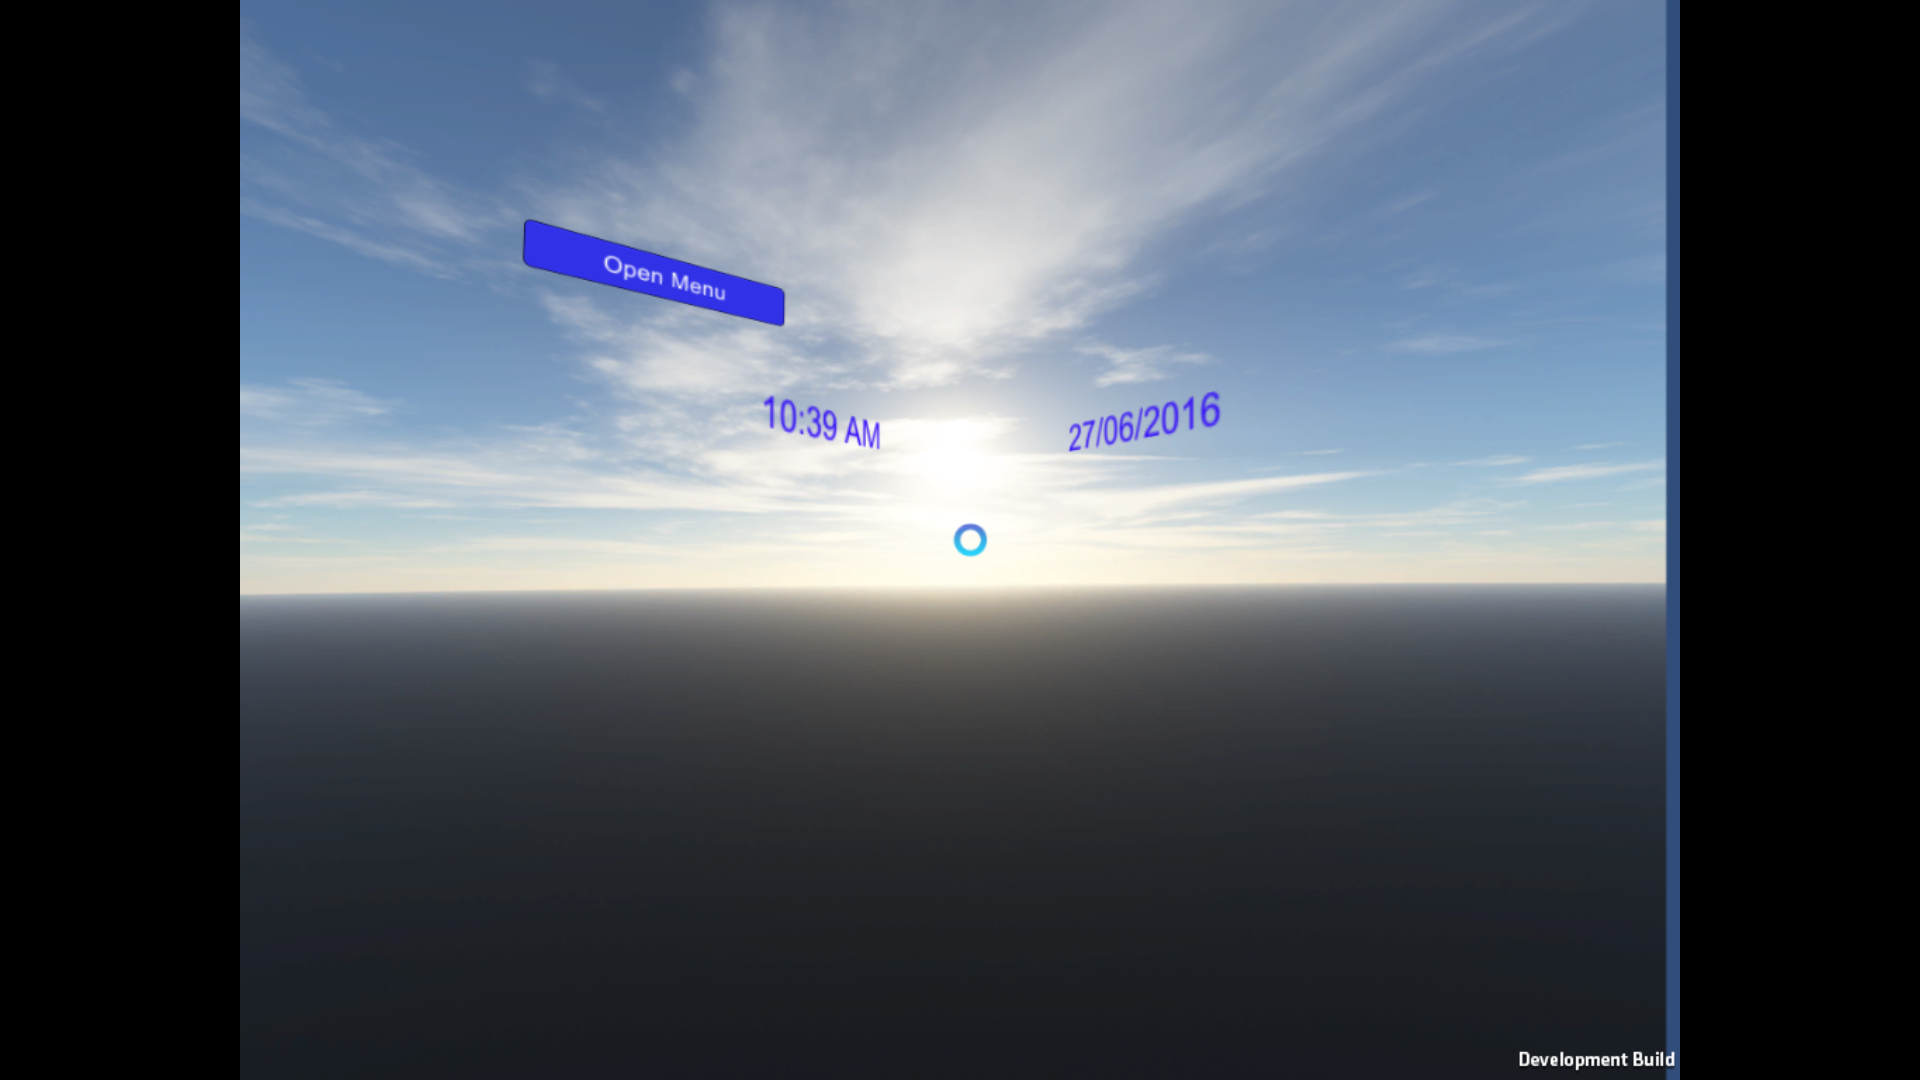
\includegraphics[width=\textwidth]{images/inicio.png} 
  \caption{Pantalla de inicio del sistema.}
  \label{fig:init1}
\end{figure}

\begin{figure} [H]
\centering	
	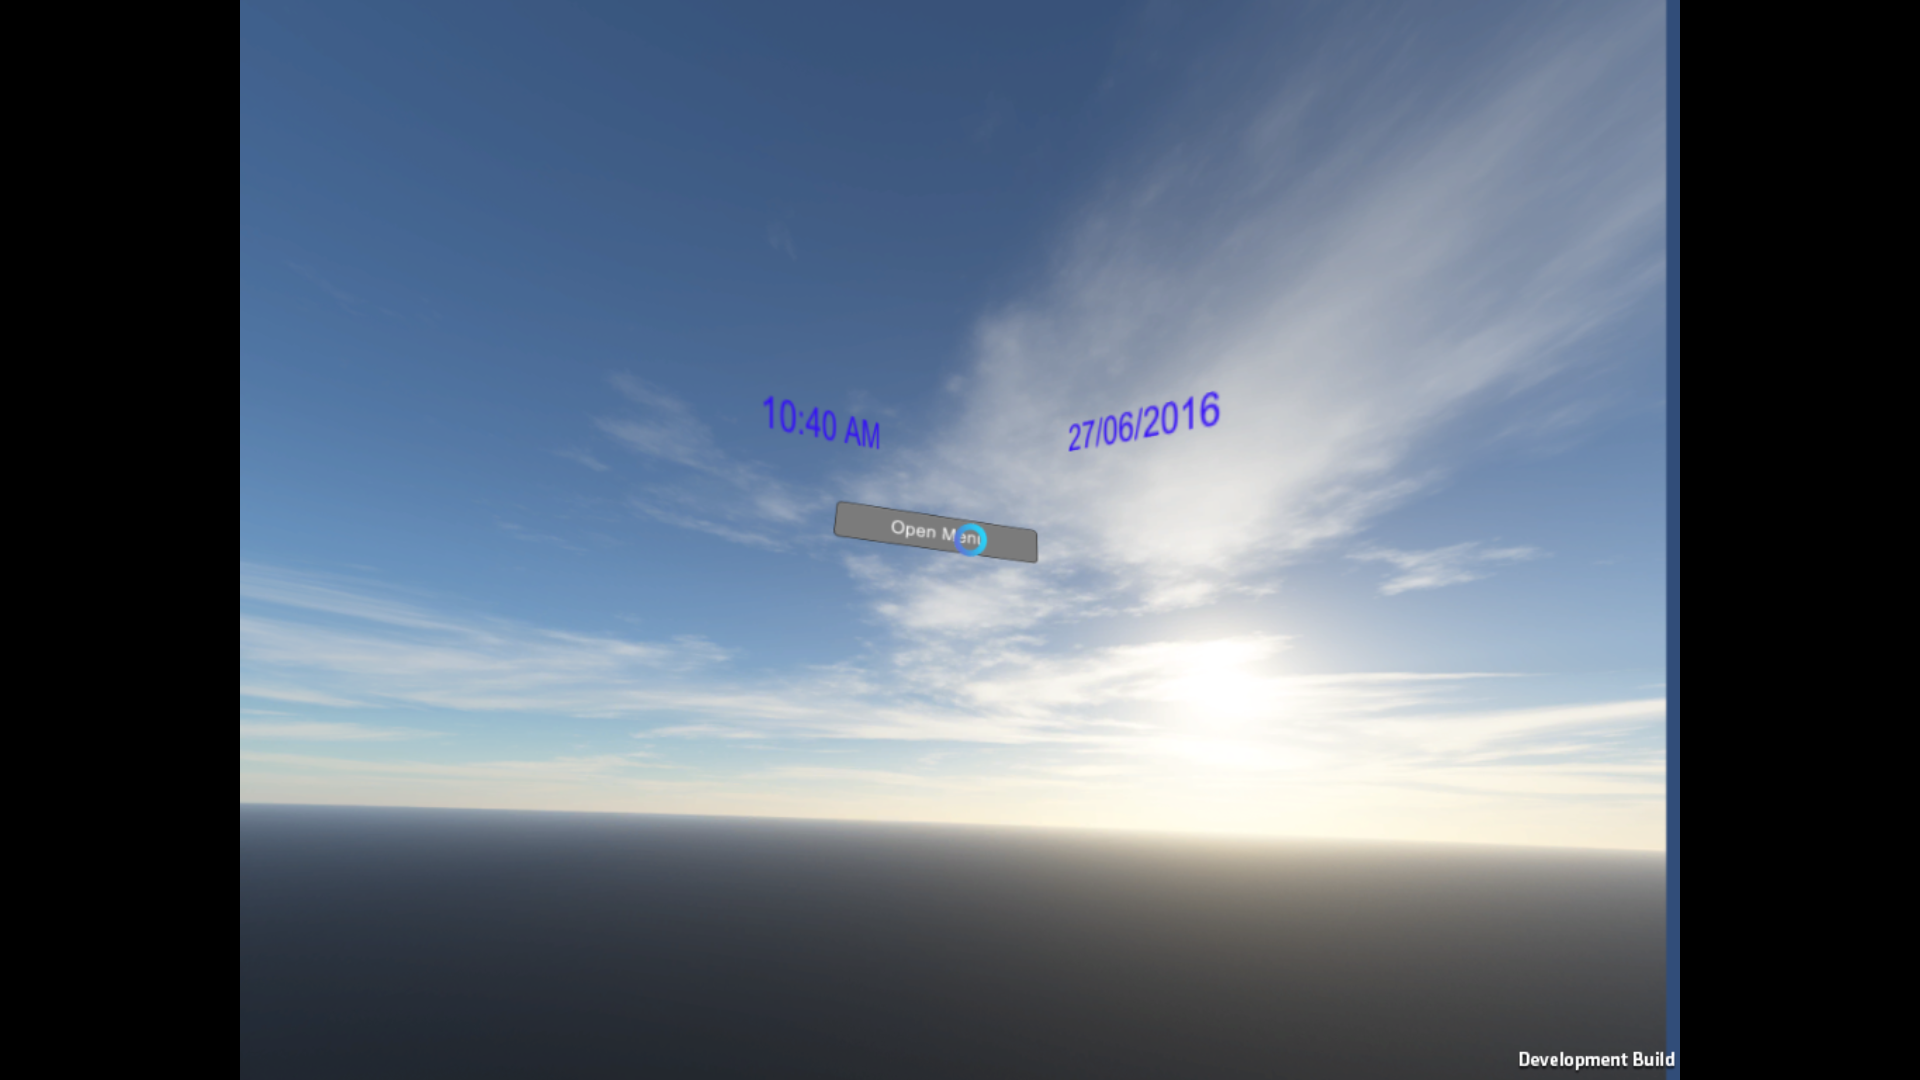
\includegraphics[width=\textwidth]{images/int_menu_open.png} 
  \caption{Usuario seleccionado la opci�n para abrir el men�.}
  \label{fig:openMenu1}
\end{figure}

\begin{figure} [H]
\centering	
	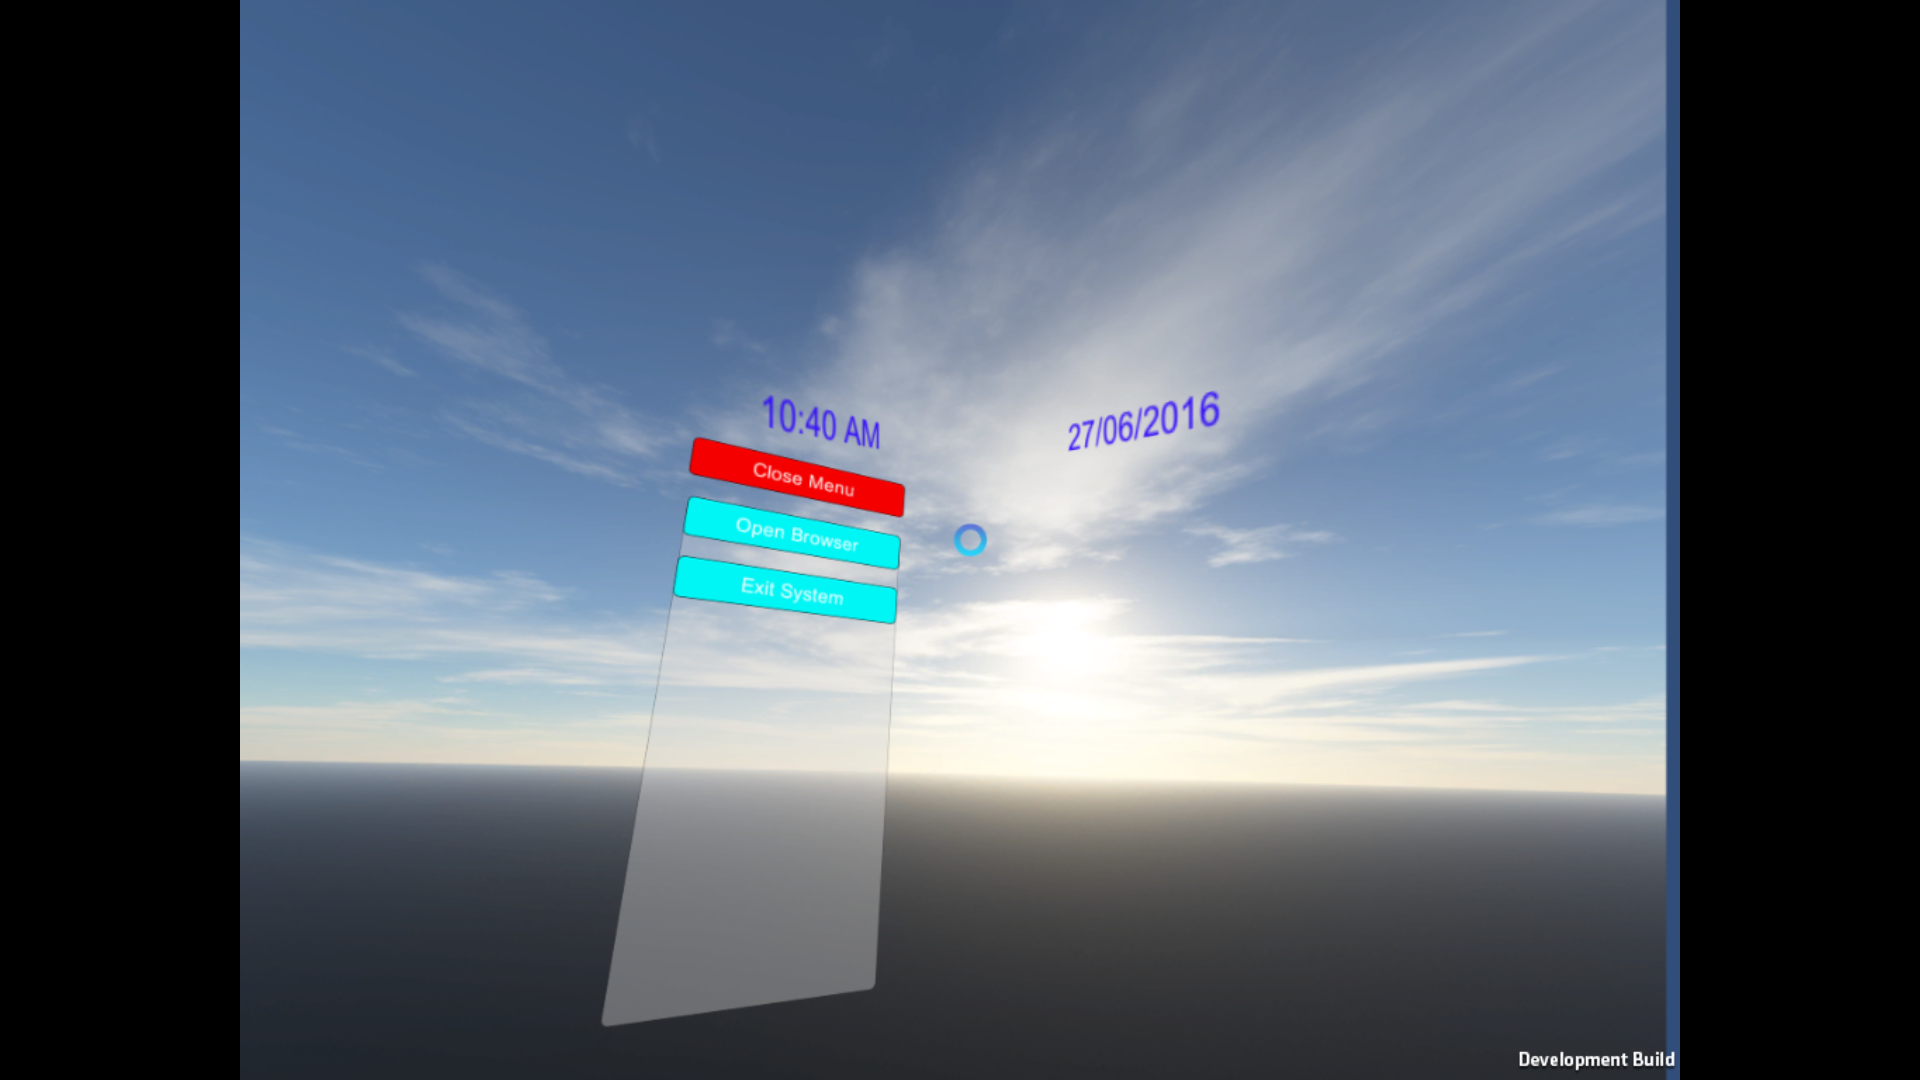
\includegraphics[width=\textwidth]{images/menu_abierto.png} 
  \caption{Men� desplegado.}
  \label{fig:menu1}
\end{figure}

\begin{figure} [H]
\centering	
	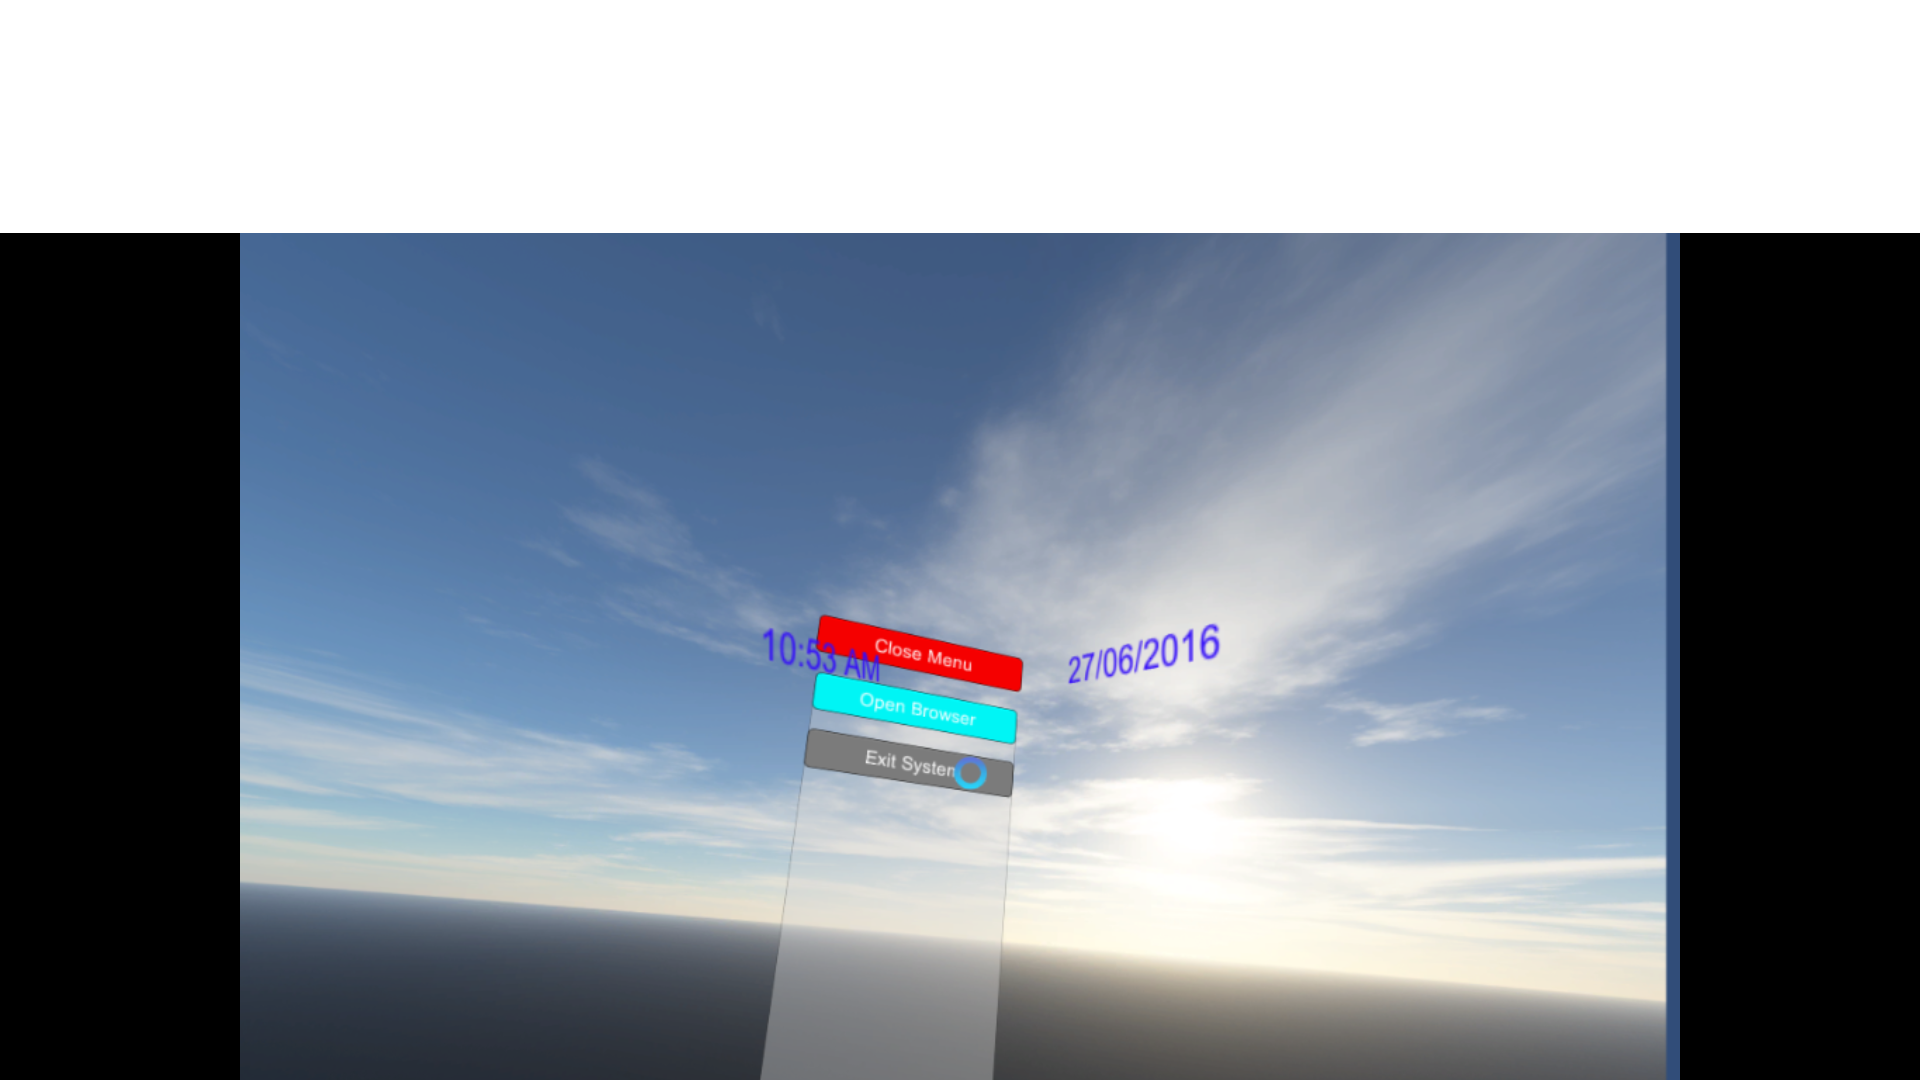
\includegraphics[width=\textwidth]{images/salir_sistema.png} 
  \caption{Usuario seleccionado la opci�n para apagar el sistema.}
  \label{fig:exit1}
\end{figure}

\lsection{Caso 2}
\label{Anexo:caso2}
Recordemos este caso de uso. El usuario debe abrir el men� desplegable y seleccionar la opci�n del navegador. Tras eso debe cerrar dicho navegador y el sistema.

\begin{figure} [H]
\centering	
	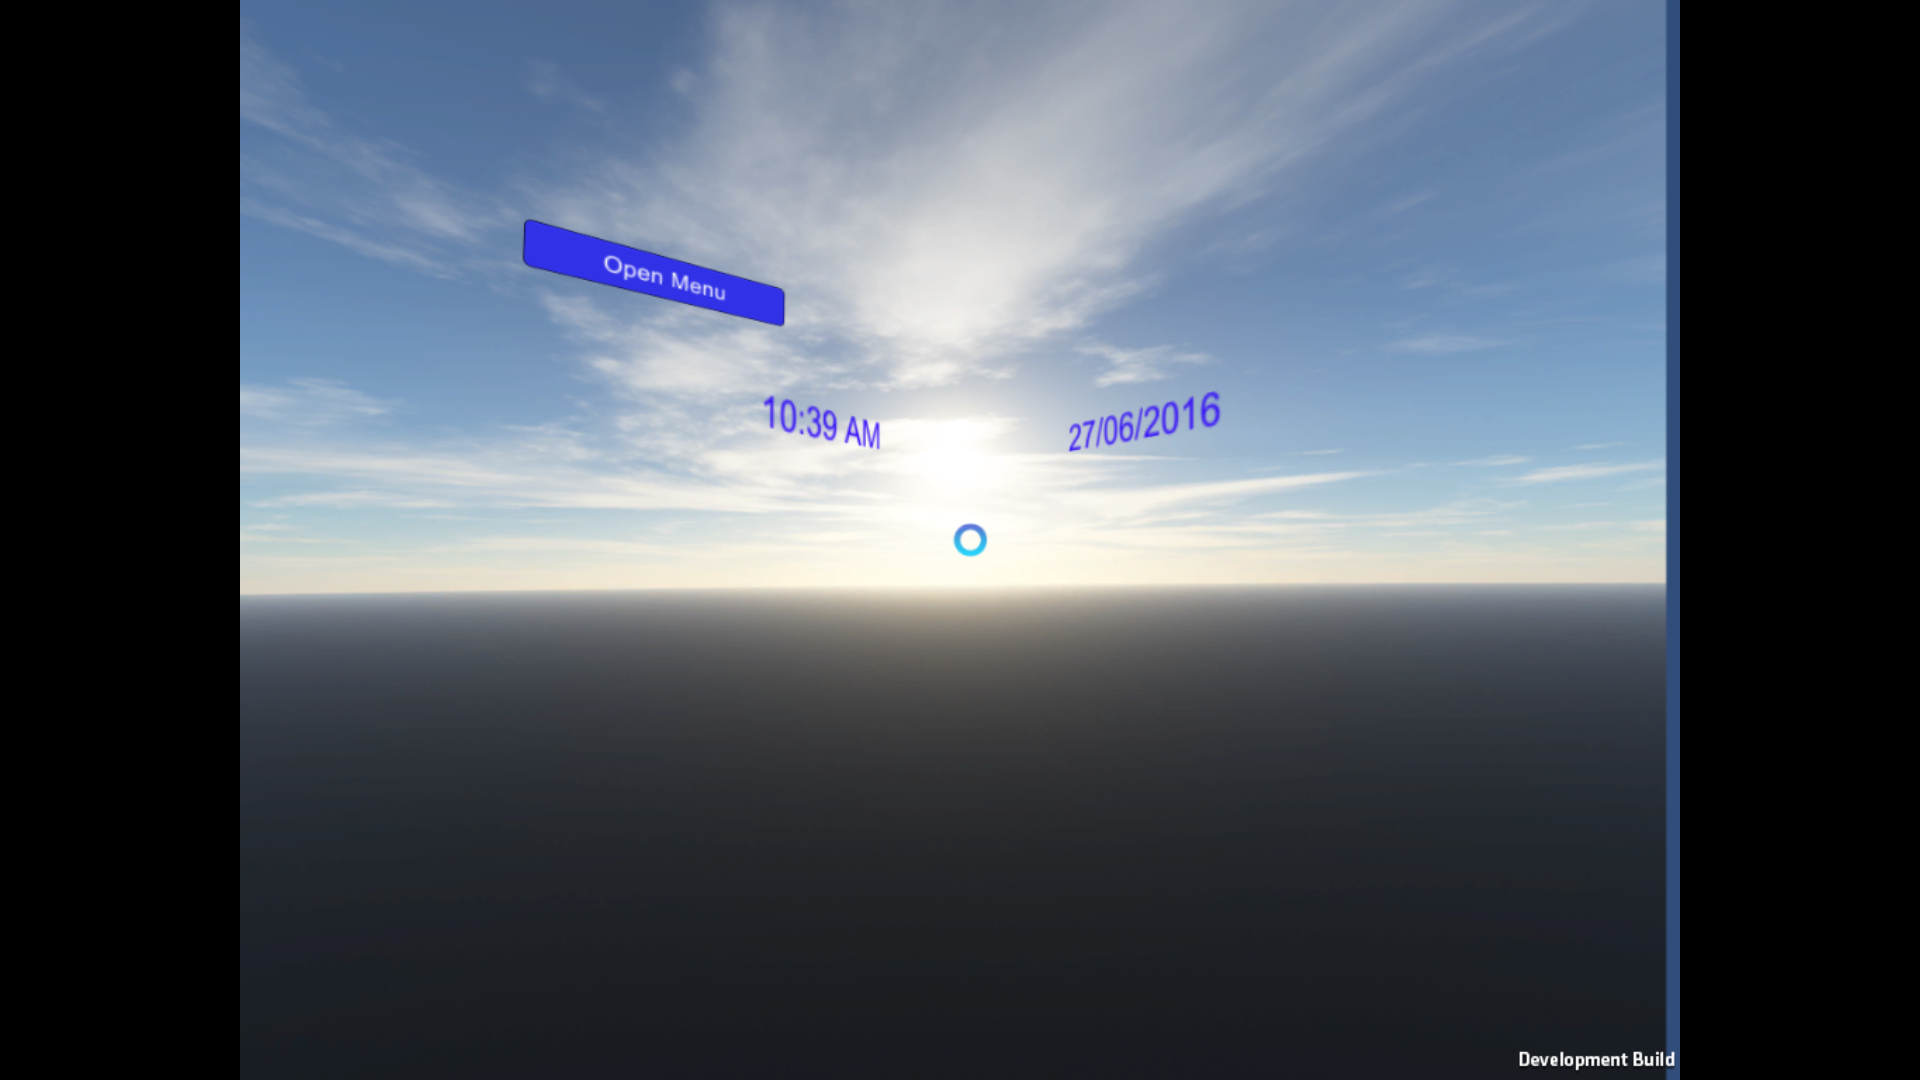
\includegraphics[width=\textwidth]{images/inicio.png} 
  \caption{Pantalla de inicio del sistema.}
  \label{fig:init2}
\end{figure}

\begin{figure} [H]
\centering	
	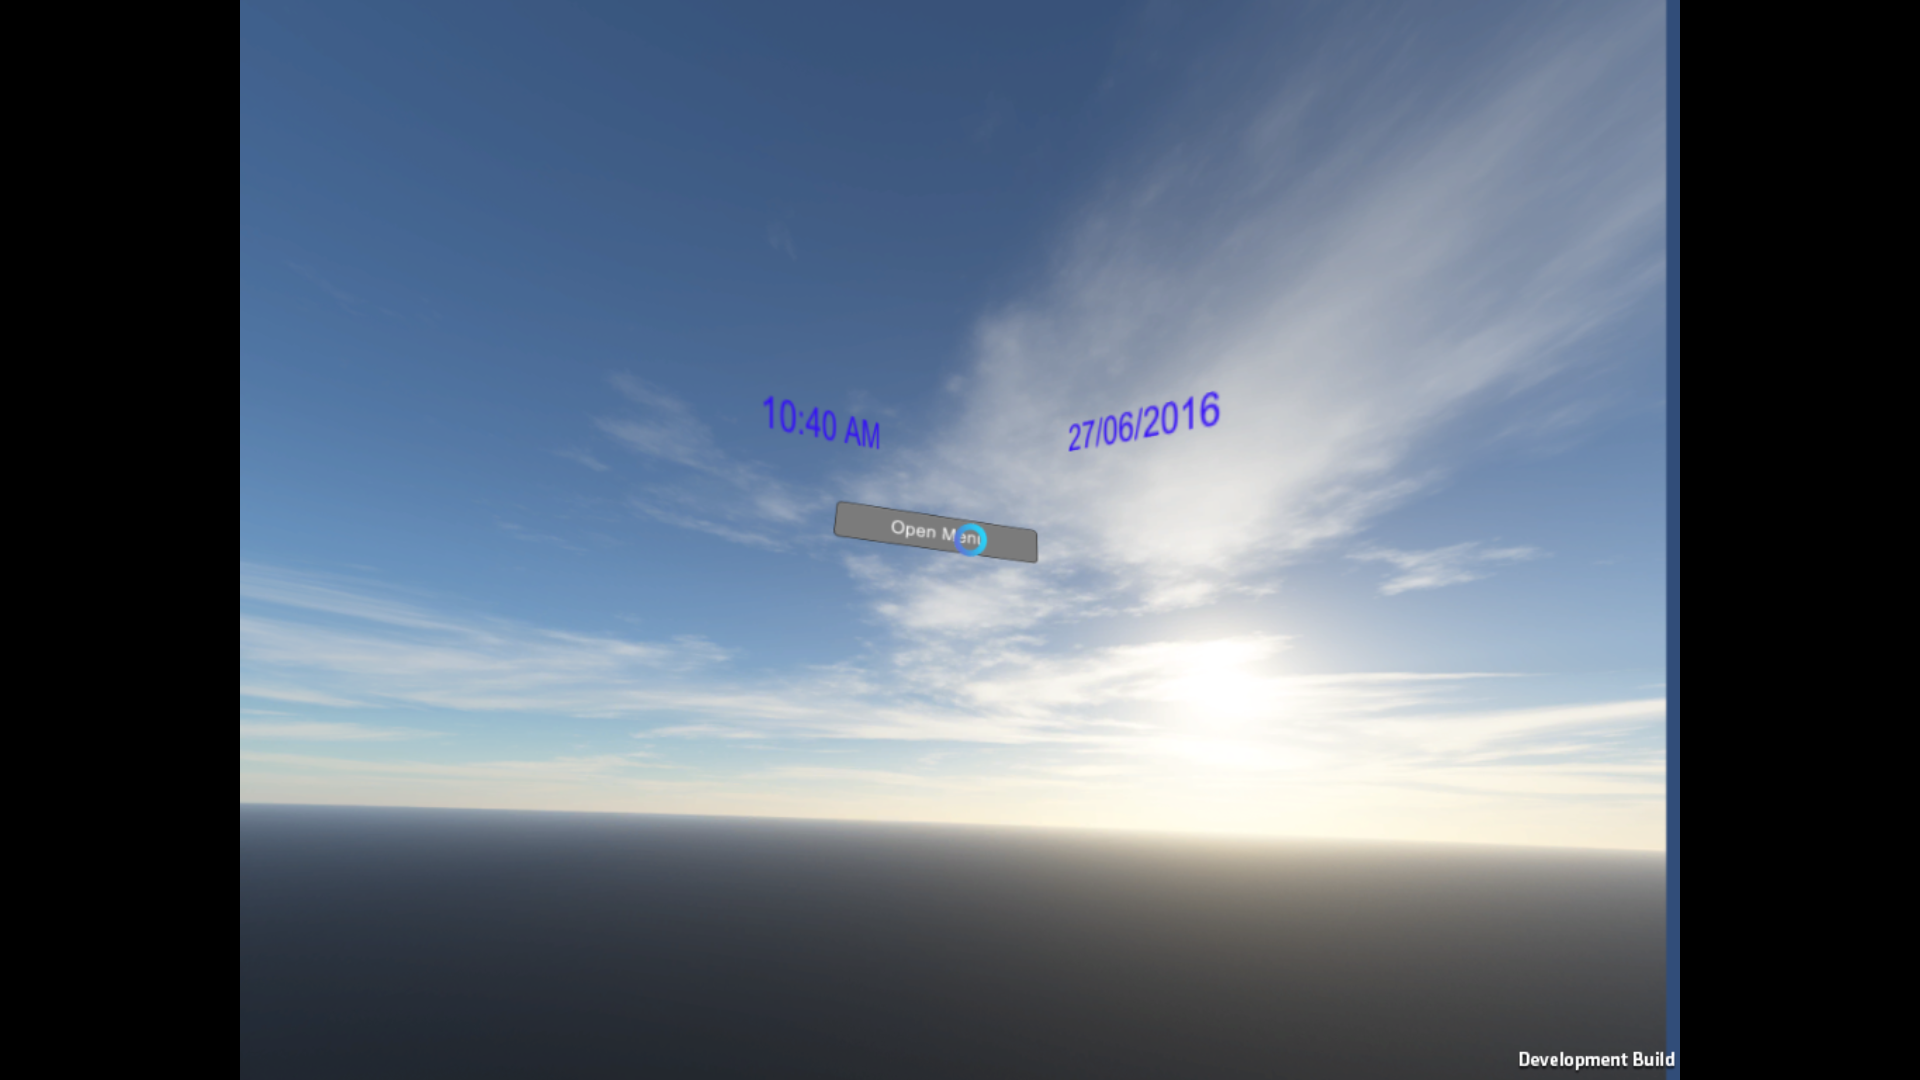
\includegraphics[width=\textwidth]{images/int_menu_open.png} 
  \caption{Usuario seleccionado la opci�n para abrir el men�.}
  \label{fig:openMenu2}
\end{figure}

\begin{figure} [H]
\centering	
	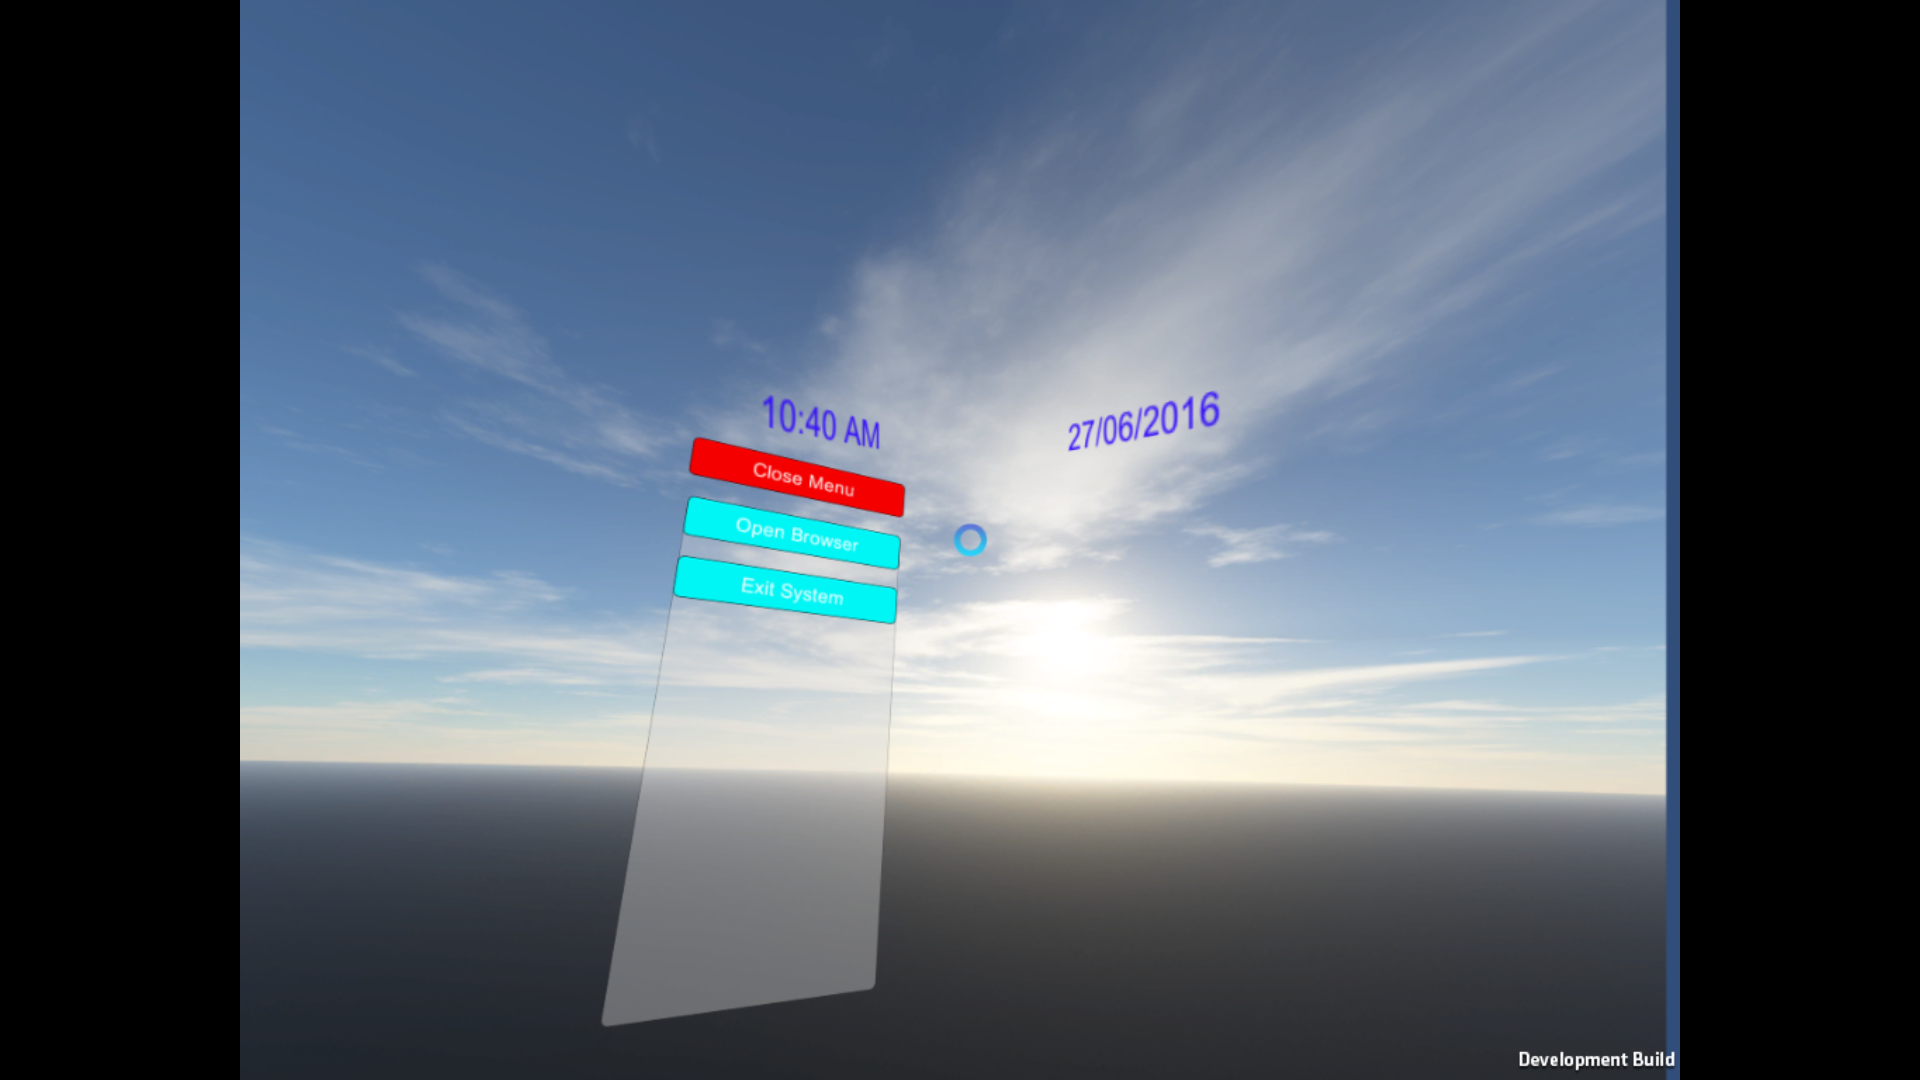
\includegraphics[width=\textwidth]{images/menu_abierto.png} 
  \caption{Men� desplegado.}
  \label{fig:menu2}
\end{figure}

\begin{figure} [H]
\centering	
	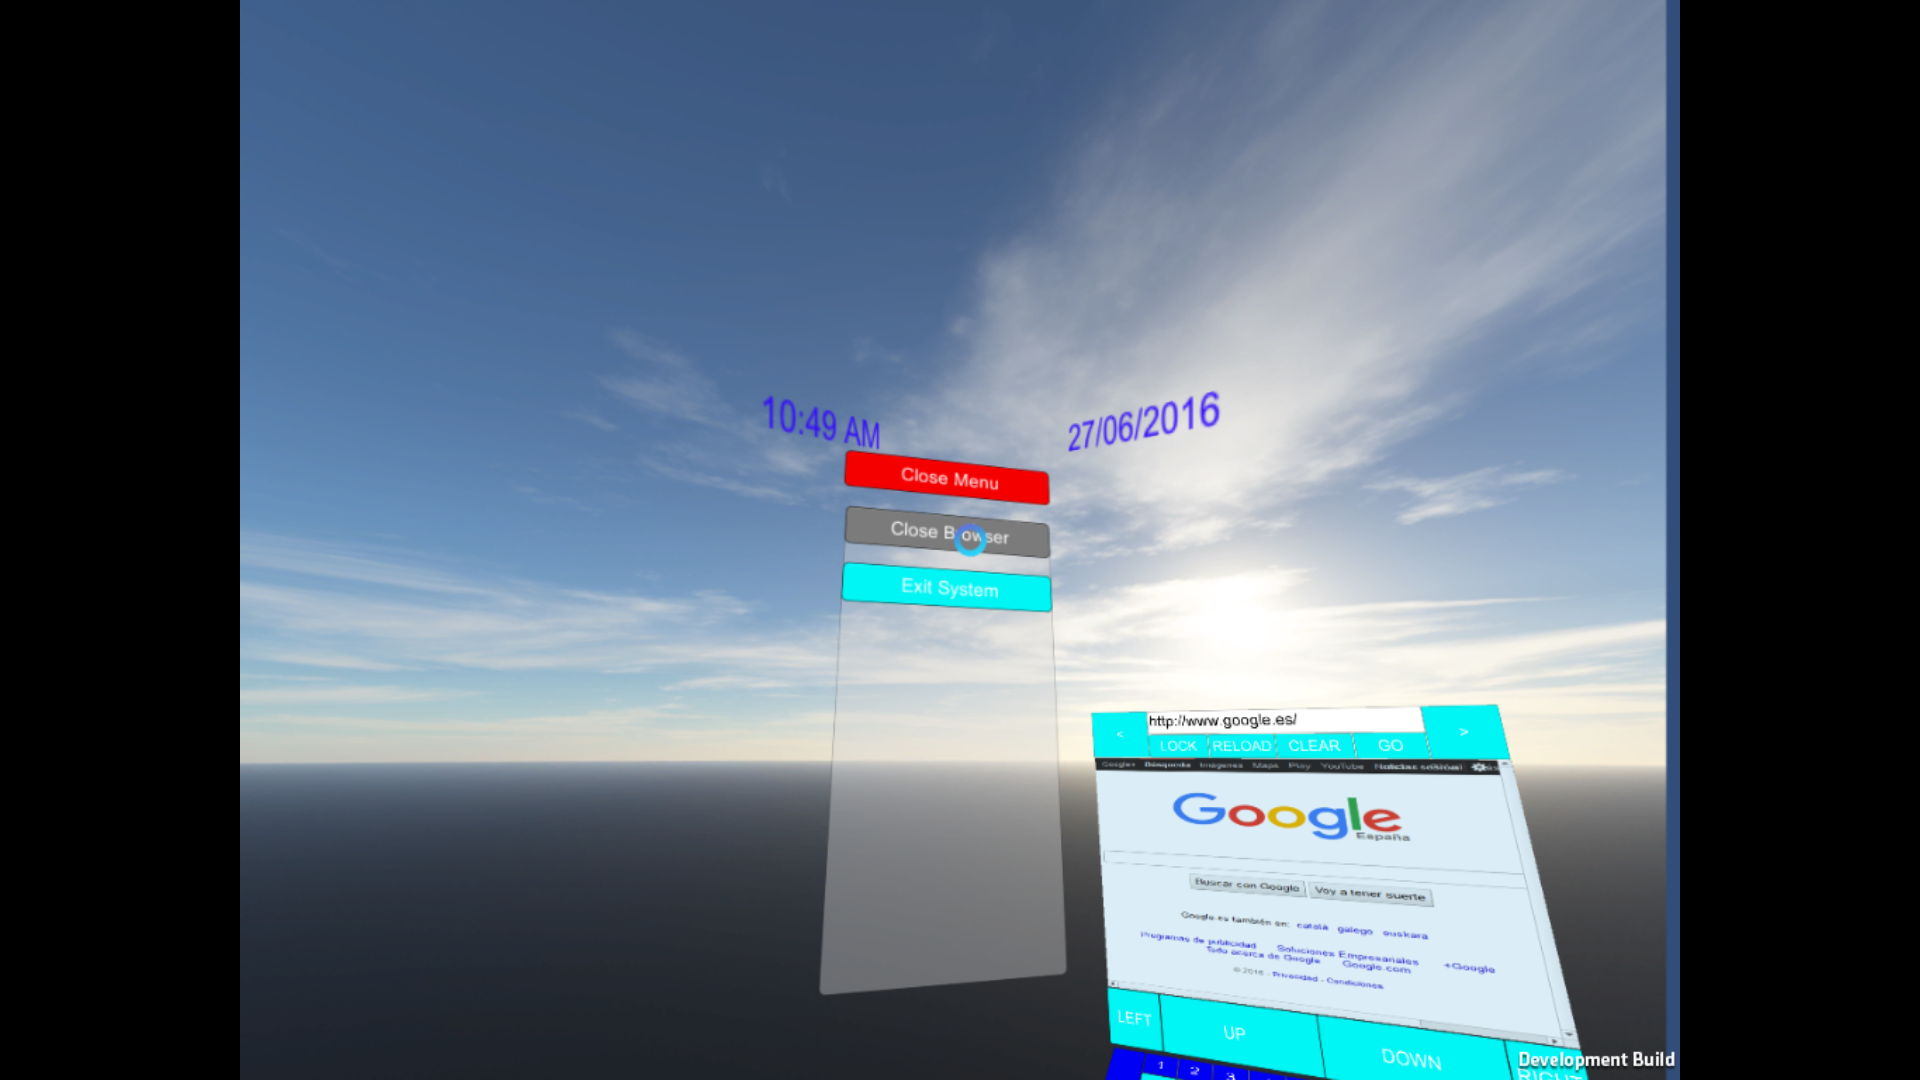
\includegraphics[width=\textwidth]{images/Apertura_browser.png} 
  \caption{Usuario seleccionando la opci�n para abrir el navegador.}
  \label{fig:initBrowser1}
\end{figure}

\begin{figure} [H]
\centering	
	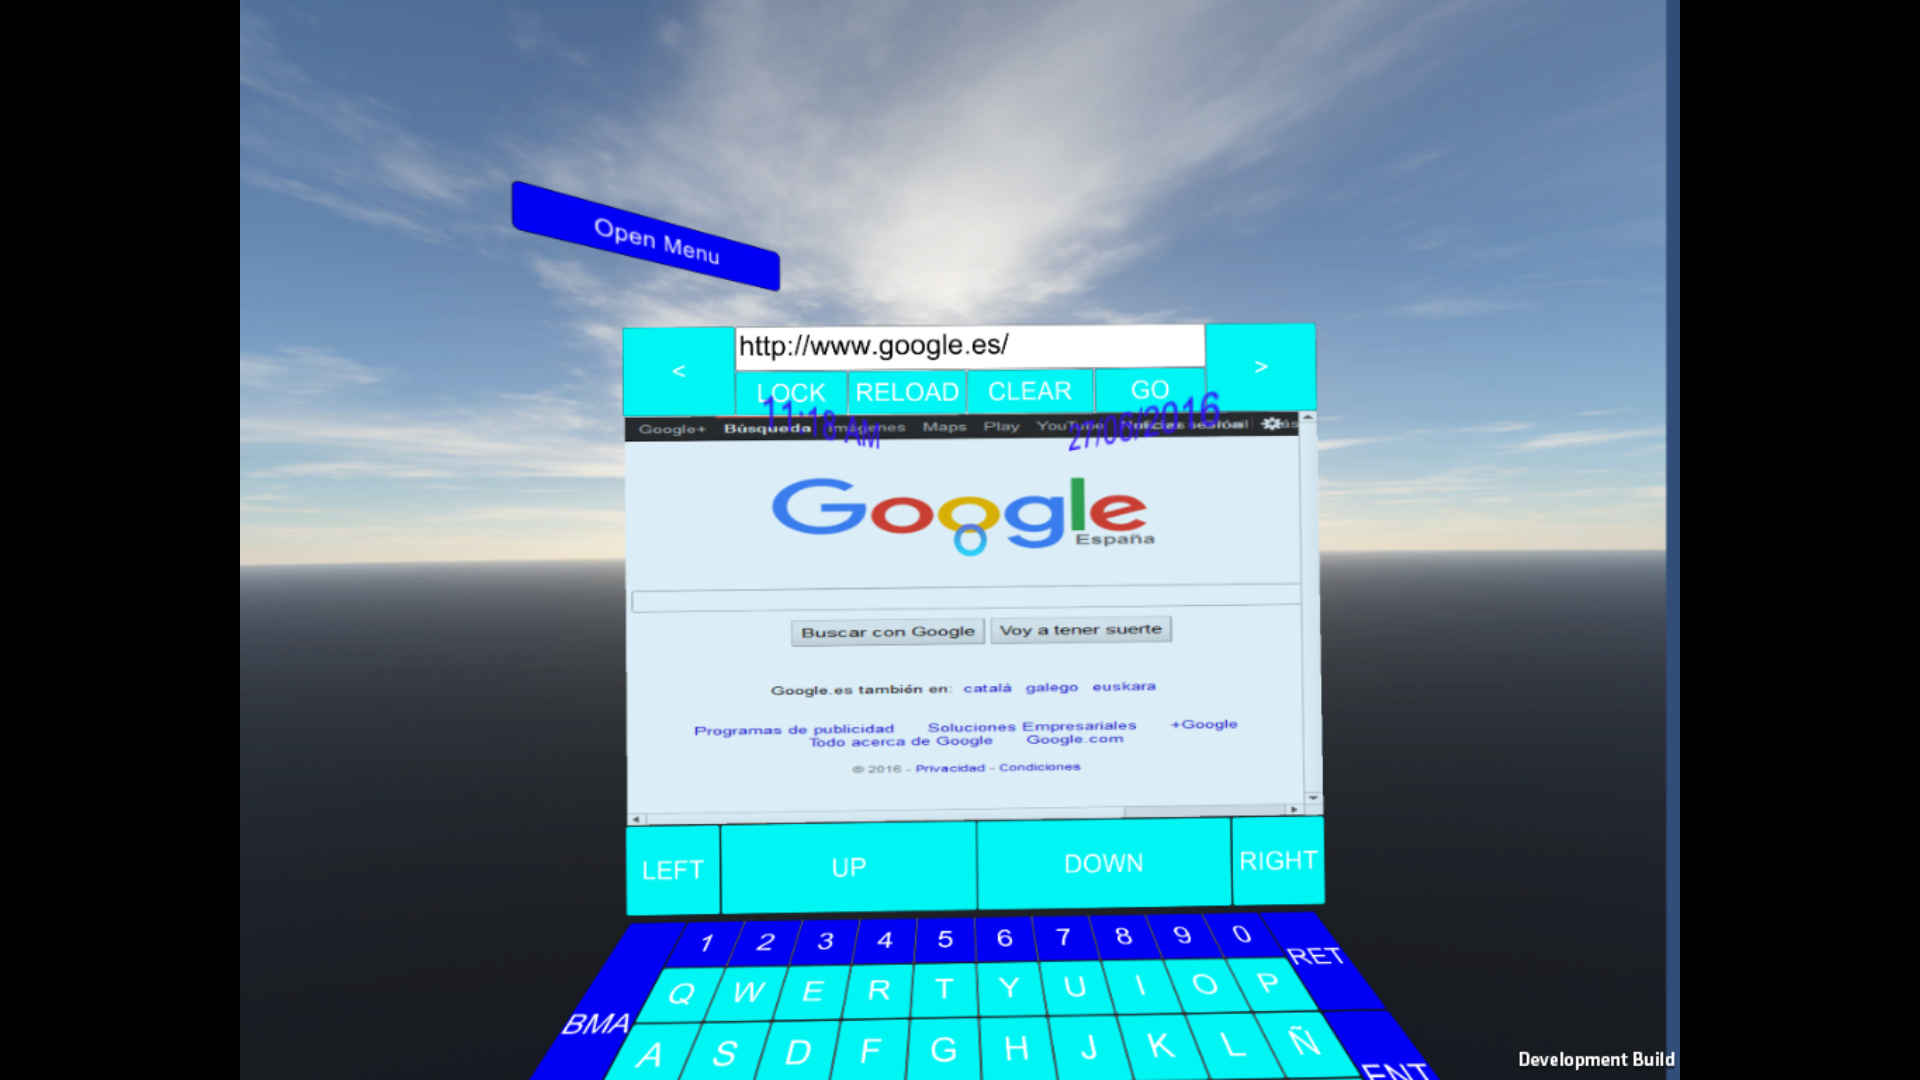
\includegraphics[width=\textwidth]{images/browser.png} 
  \caption{Navegador del sistema.}
  \label{fig:browser1}
\end{figure}


\begin{figure} [H]
\centering	
	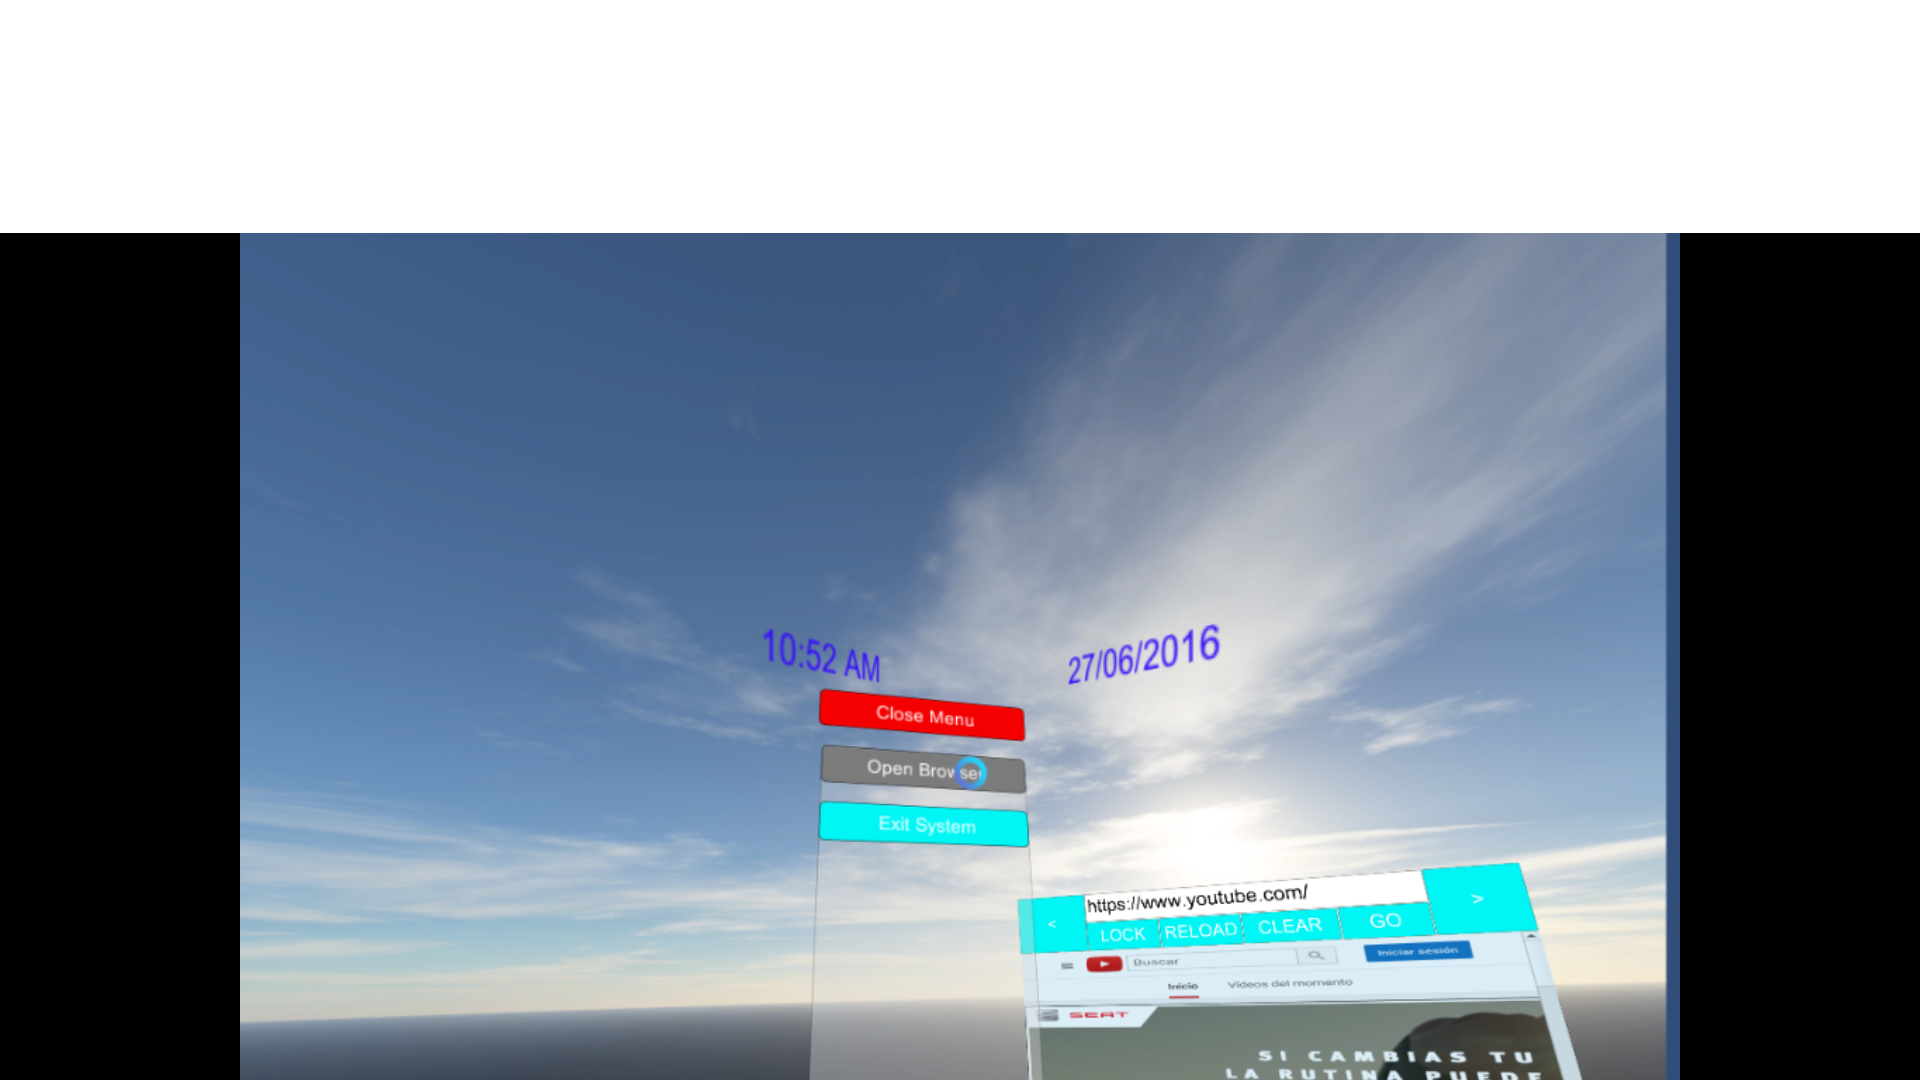
\includegraphics[width=\textwidth]{images/cierre_navegador.png} 
  \caption{Usuario seleccionado la opci�n para cerrar el navegador.}
  \label{fig:exitBrowser1}
\end{figure}

\begin{figure} [H]
\centering	
	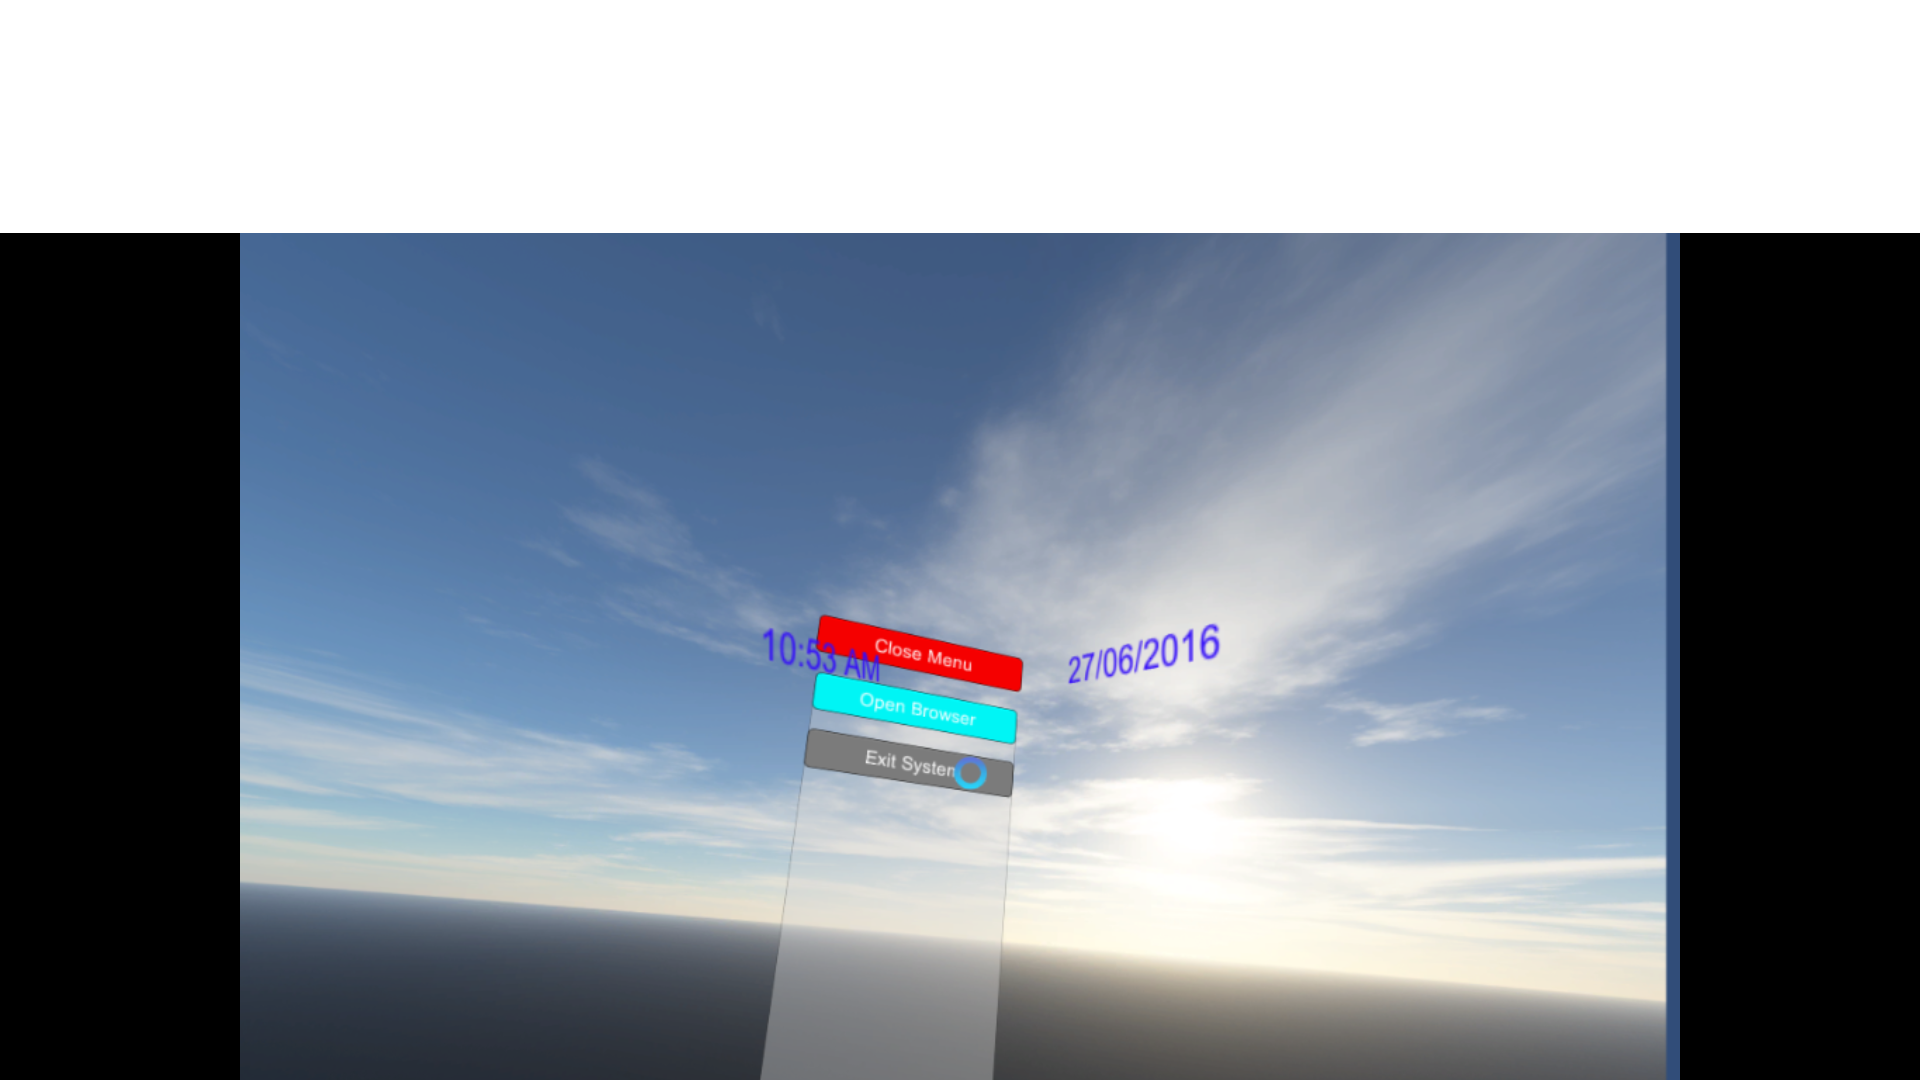
\includegraphics[width=\textwidth]{images/salir_sistema.png} 
  \caption{Usuario seleccionado la opci�n para apagar el sistema}
  \label{fig:exit2}
\end{figure}

\lsection{Caso 3}
\label{Anexo:caso3}
Recordemos este caso de uso. El usuario debe abrir el men� desplegable y seleccionar la opci�n del navegador. A posterior� debe introducir la URL \url{www.youtube.es}, cargar la p�gina, seleccionar el primer v�deo que aparezca y cerrar todo el sistema.

\begin{figure} [H]
\centering	
	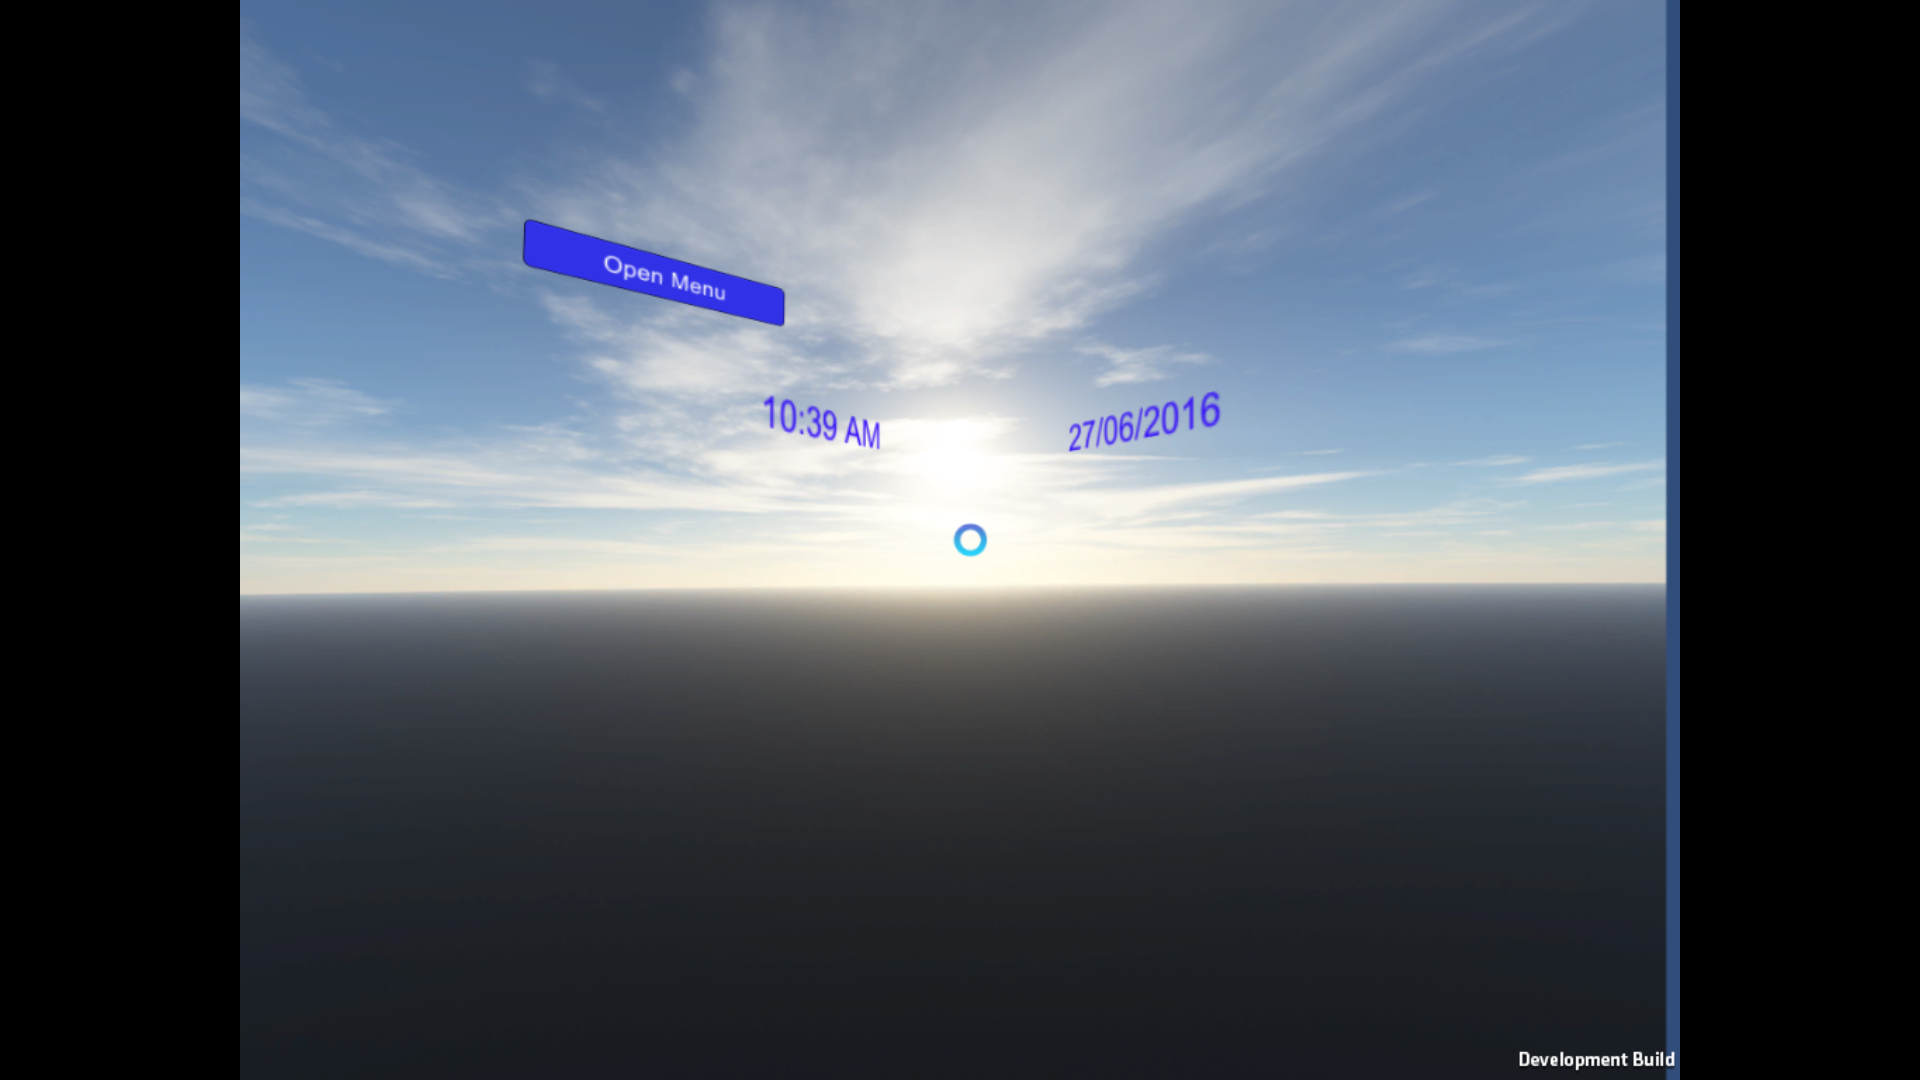
\includegraphics[width=\textwidth]{images/inicio.png} 
  \caption{Pantalla de inicio del sistema.}
  \label{fig:init3}
\end{figure}

\begin{figure} [H]
\centering	
	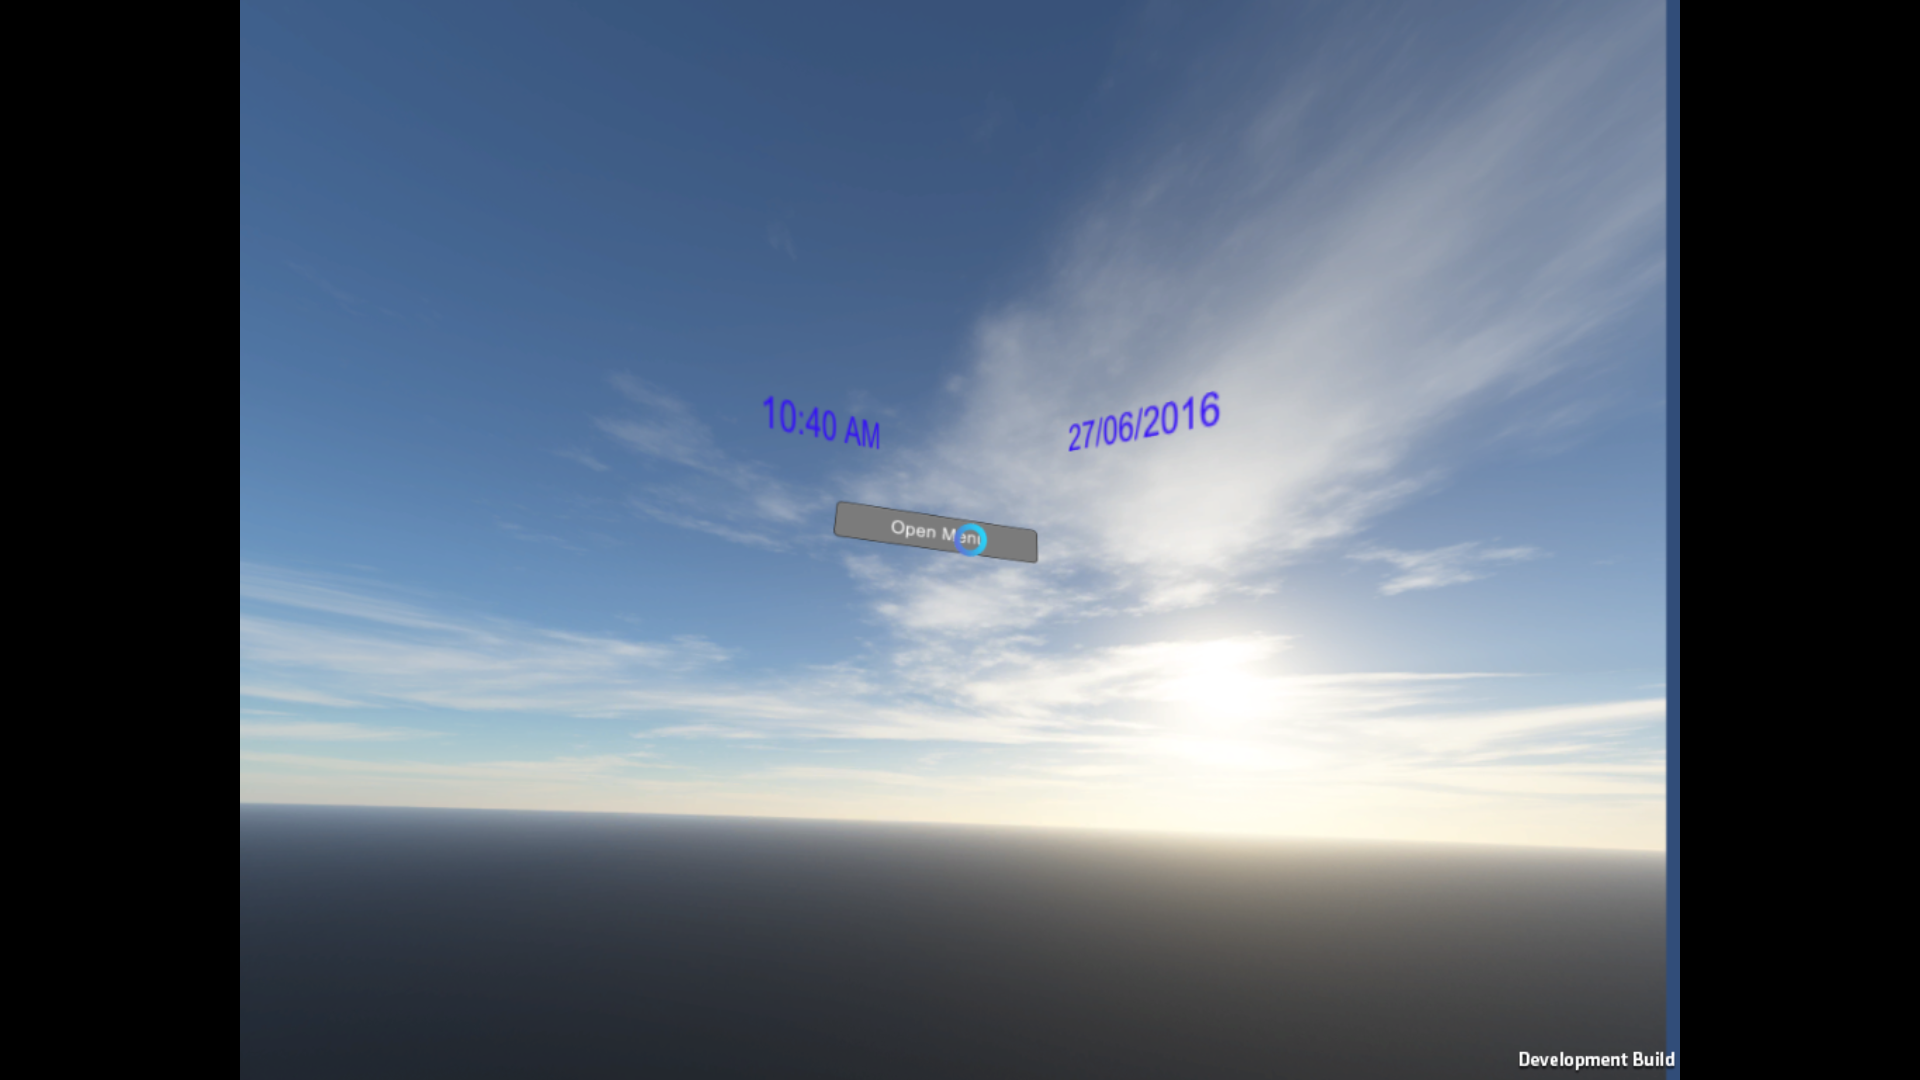
\includegraphics[width=\textwidth]{images/int_menu_open.png} 
  \caption{Usuario seleccionado la opci�n para abrir el men�.}
  \label{fig:openMenu3}
\end{figure}

\begin{figure} [H]
\centering	
	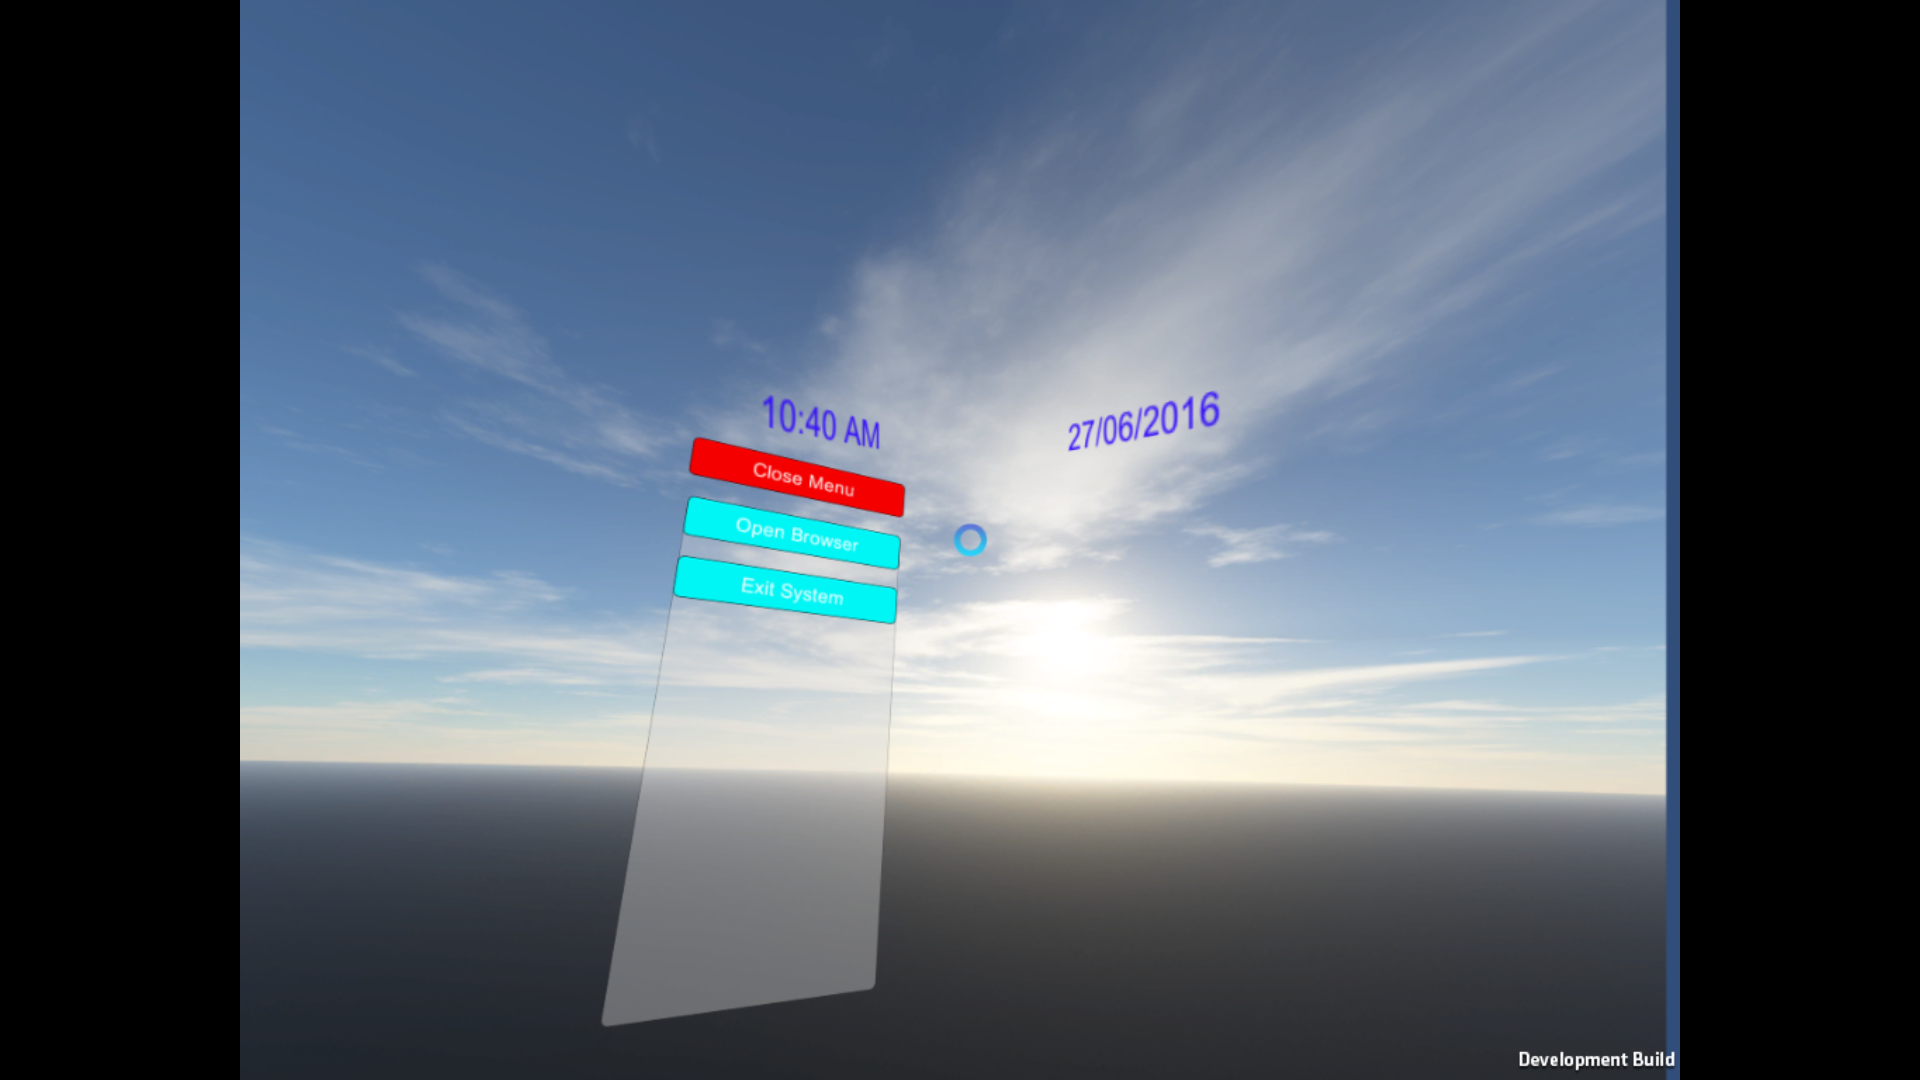
\includegraphics[width=\textwidth]{images/menu_abierto.png} 
  \caption{Men� desplegado.}
  \label{fig:menu3}
\end{figure}

\begin{figure} [H]
\centering	
	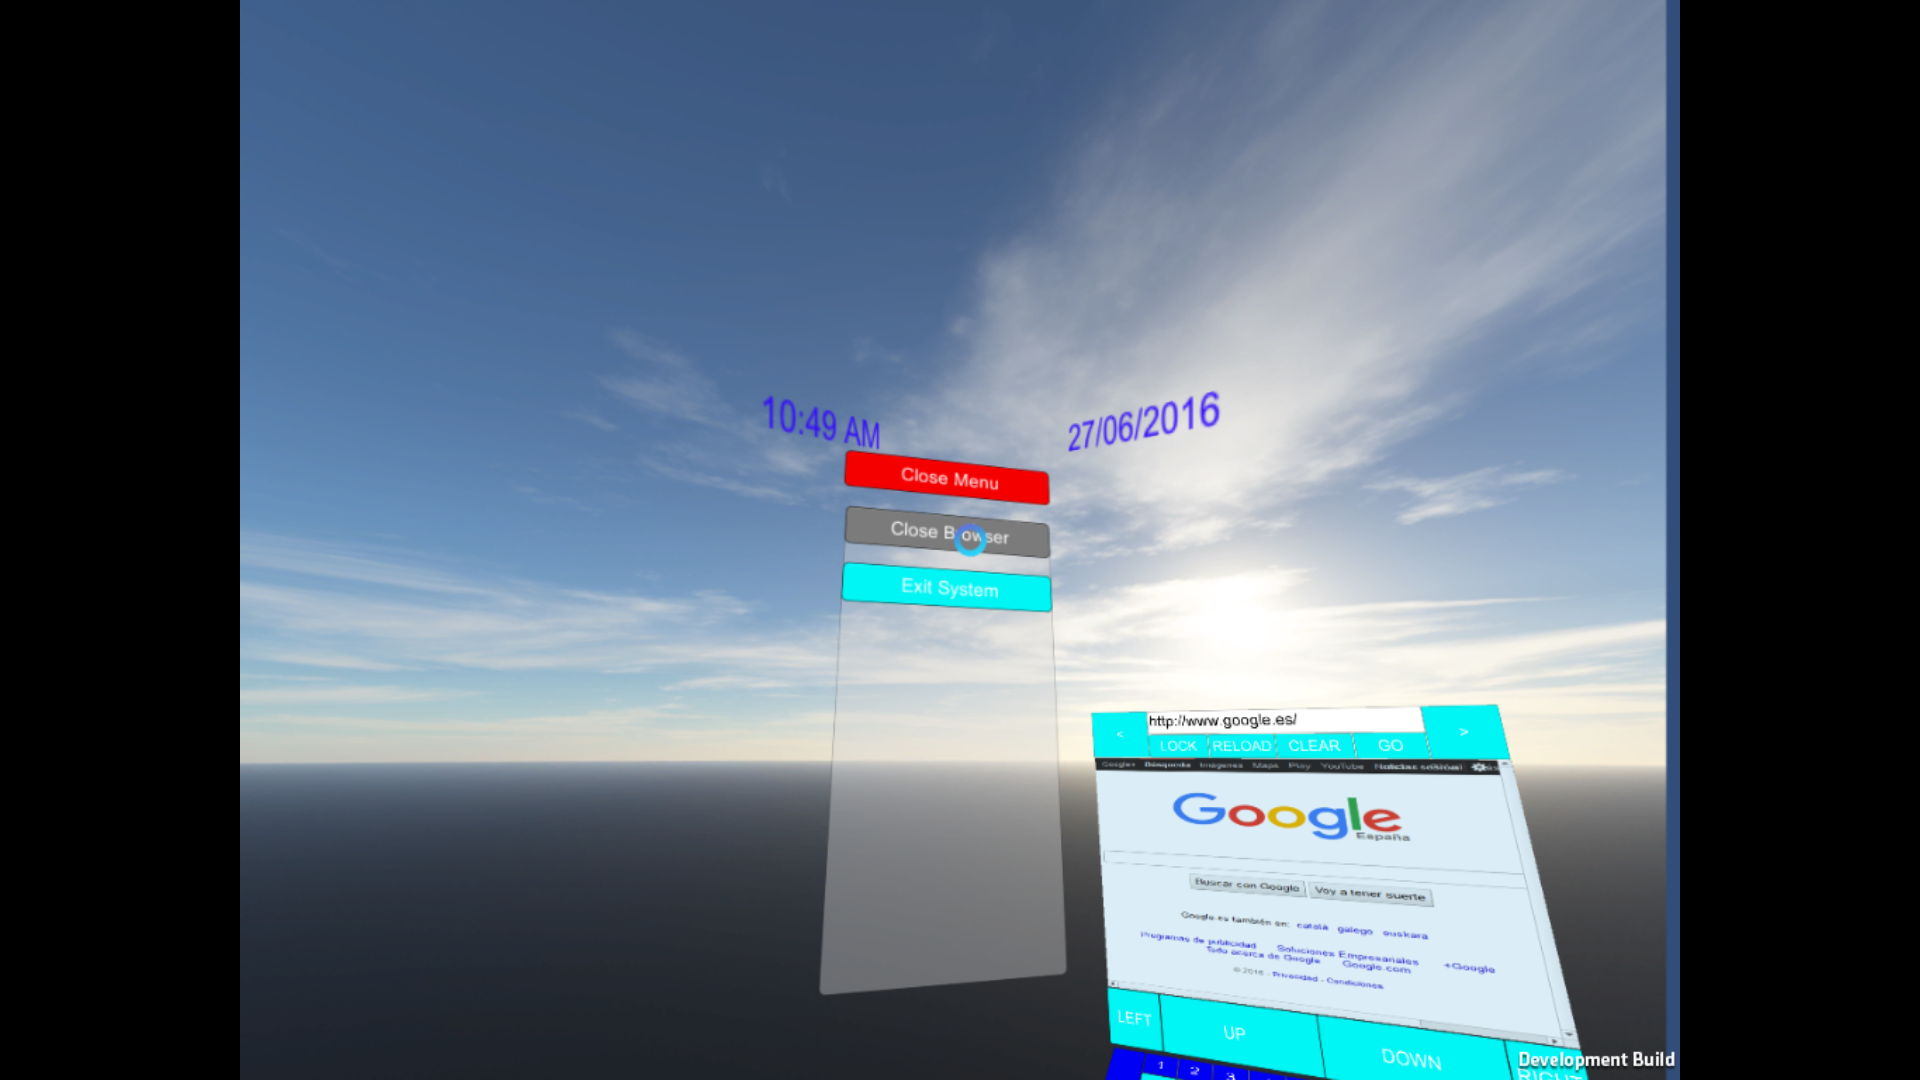
\includegraphics[width=\textwidth]{images/Apertura_browser.png} 
  \caption{Usuario seleccionando la opci�n para abrir el navegador.}
  \label{fig:initBrowser2}
\end{figure}

\begin{figure} [H]
\centering	
	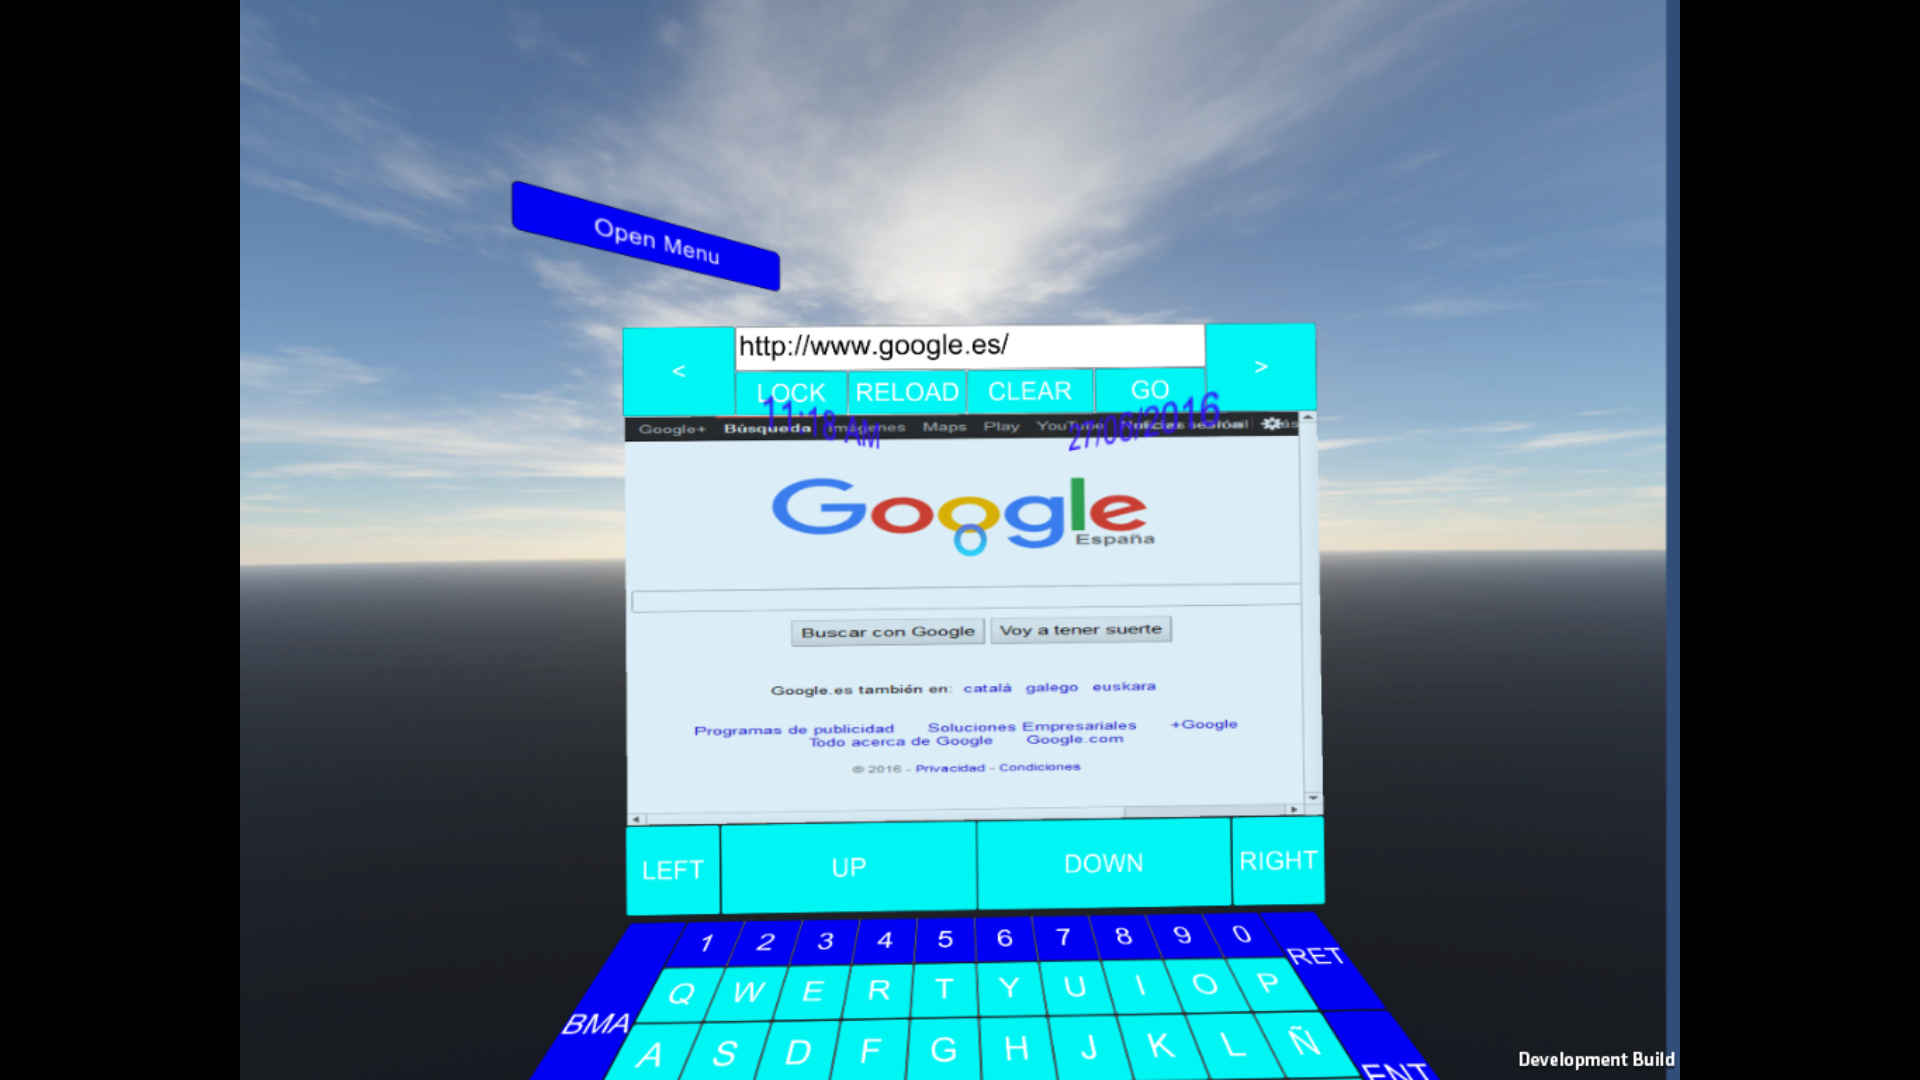
\includegraphics[width=\textwidth]{images/browser.png} 
  \caption{Navegador del sistema.}
  \label{fig:browser2}
\end{figure}

\begin{figure} [H]
\centering	
	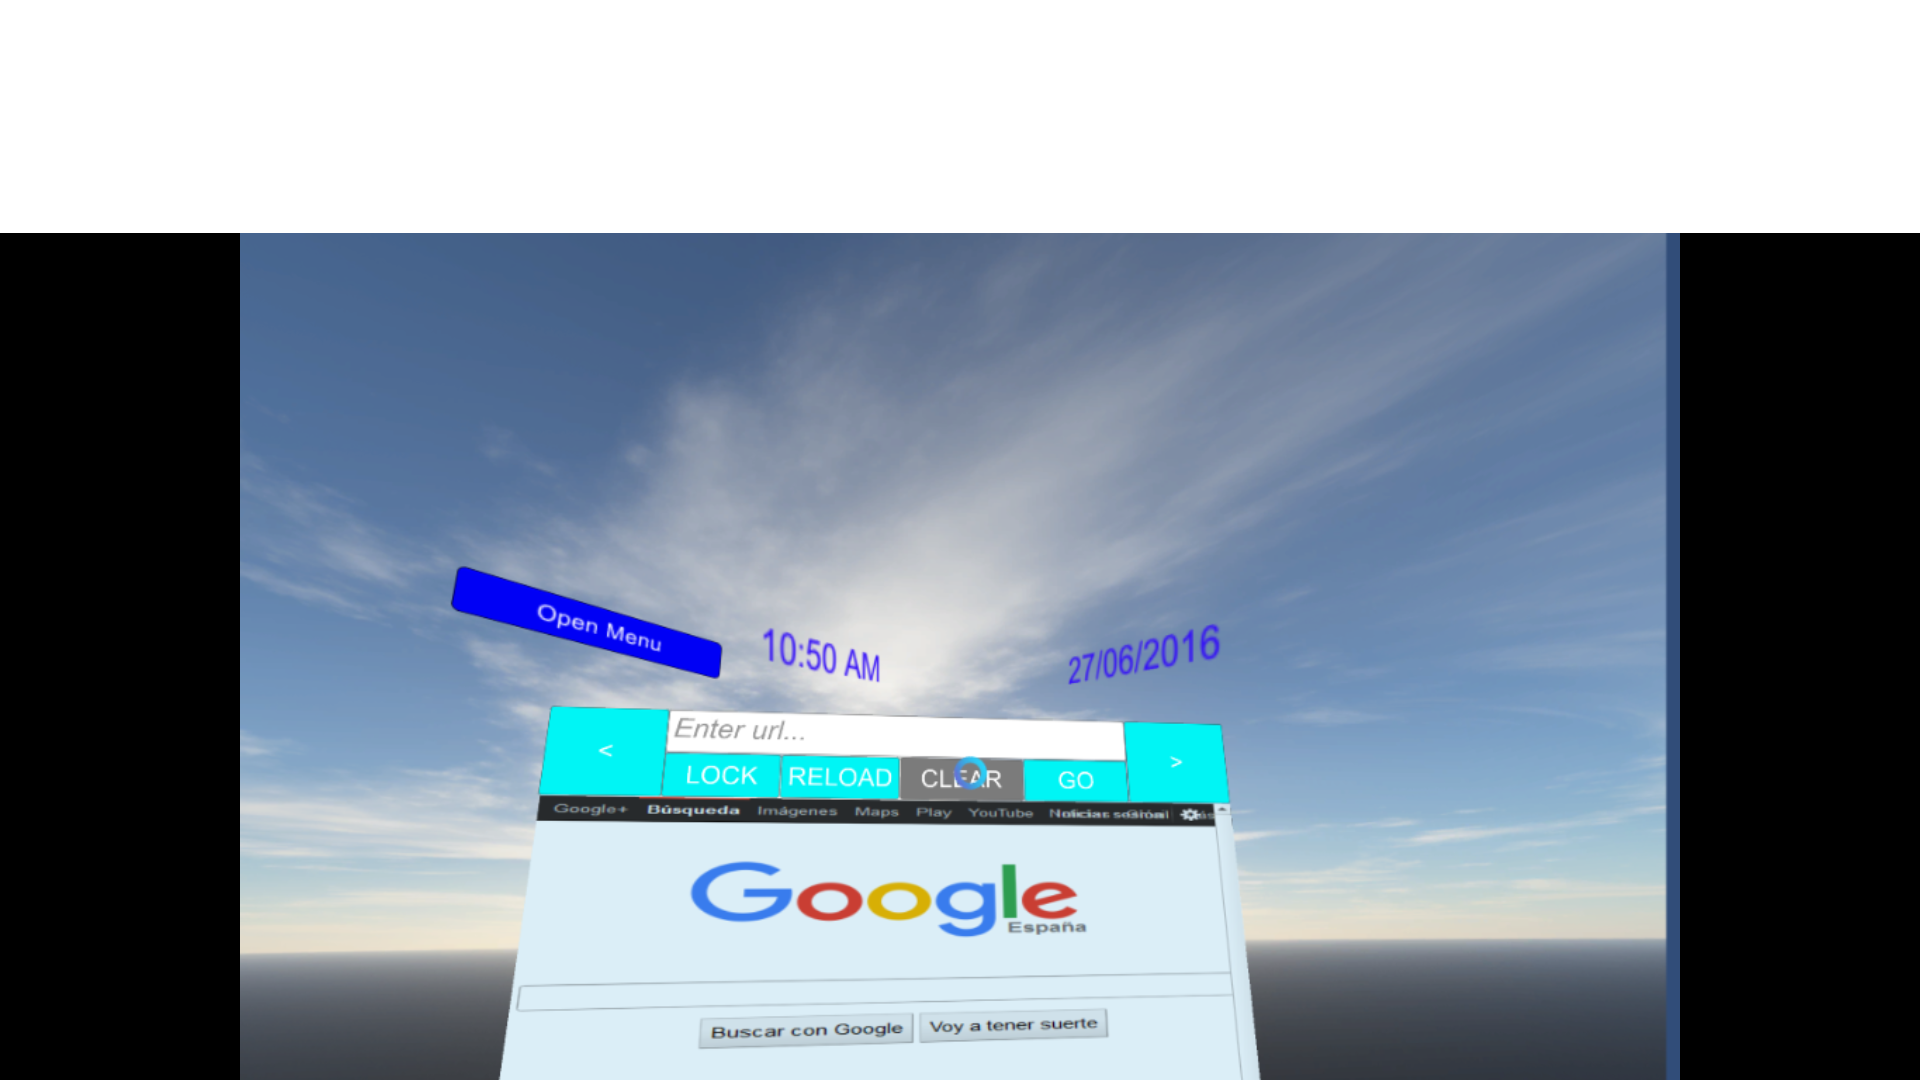
\includegraphics[width=\textwidth]{images/limpia_url.png} 
  \caption{Limpiando campo para escribir la URL.}
  \label{fig:urlClean1}
\end{figure}

\begin{figure} [H]
\centering	
	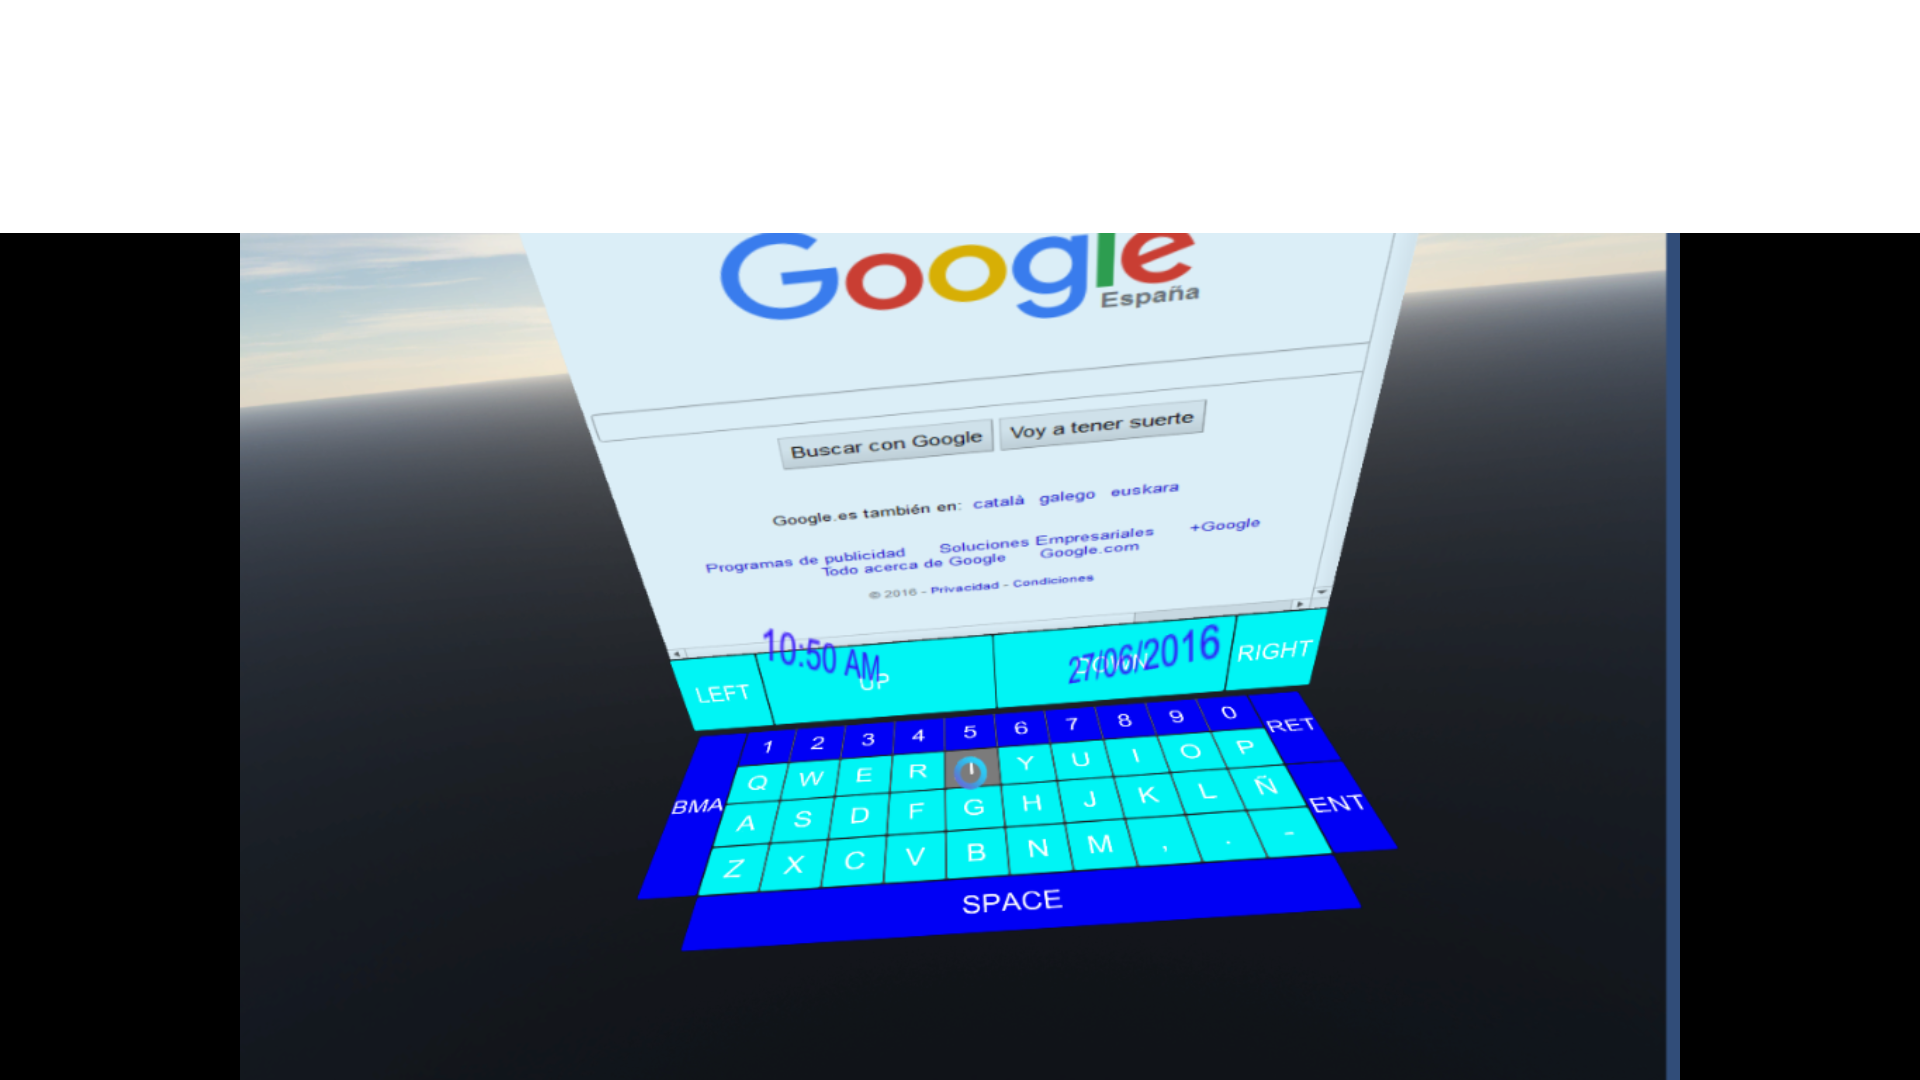
\includegraphics[width=\textwidth]{images/escritura_teclado.png} 
  \caption{Escribiendo con el teclado virtual.}
  \label{fig:writeVKB1}
\end{figure}

\begin{figure} [H]
\centering	
	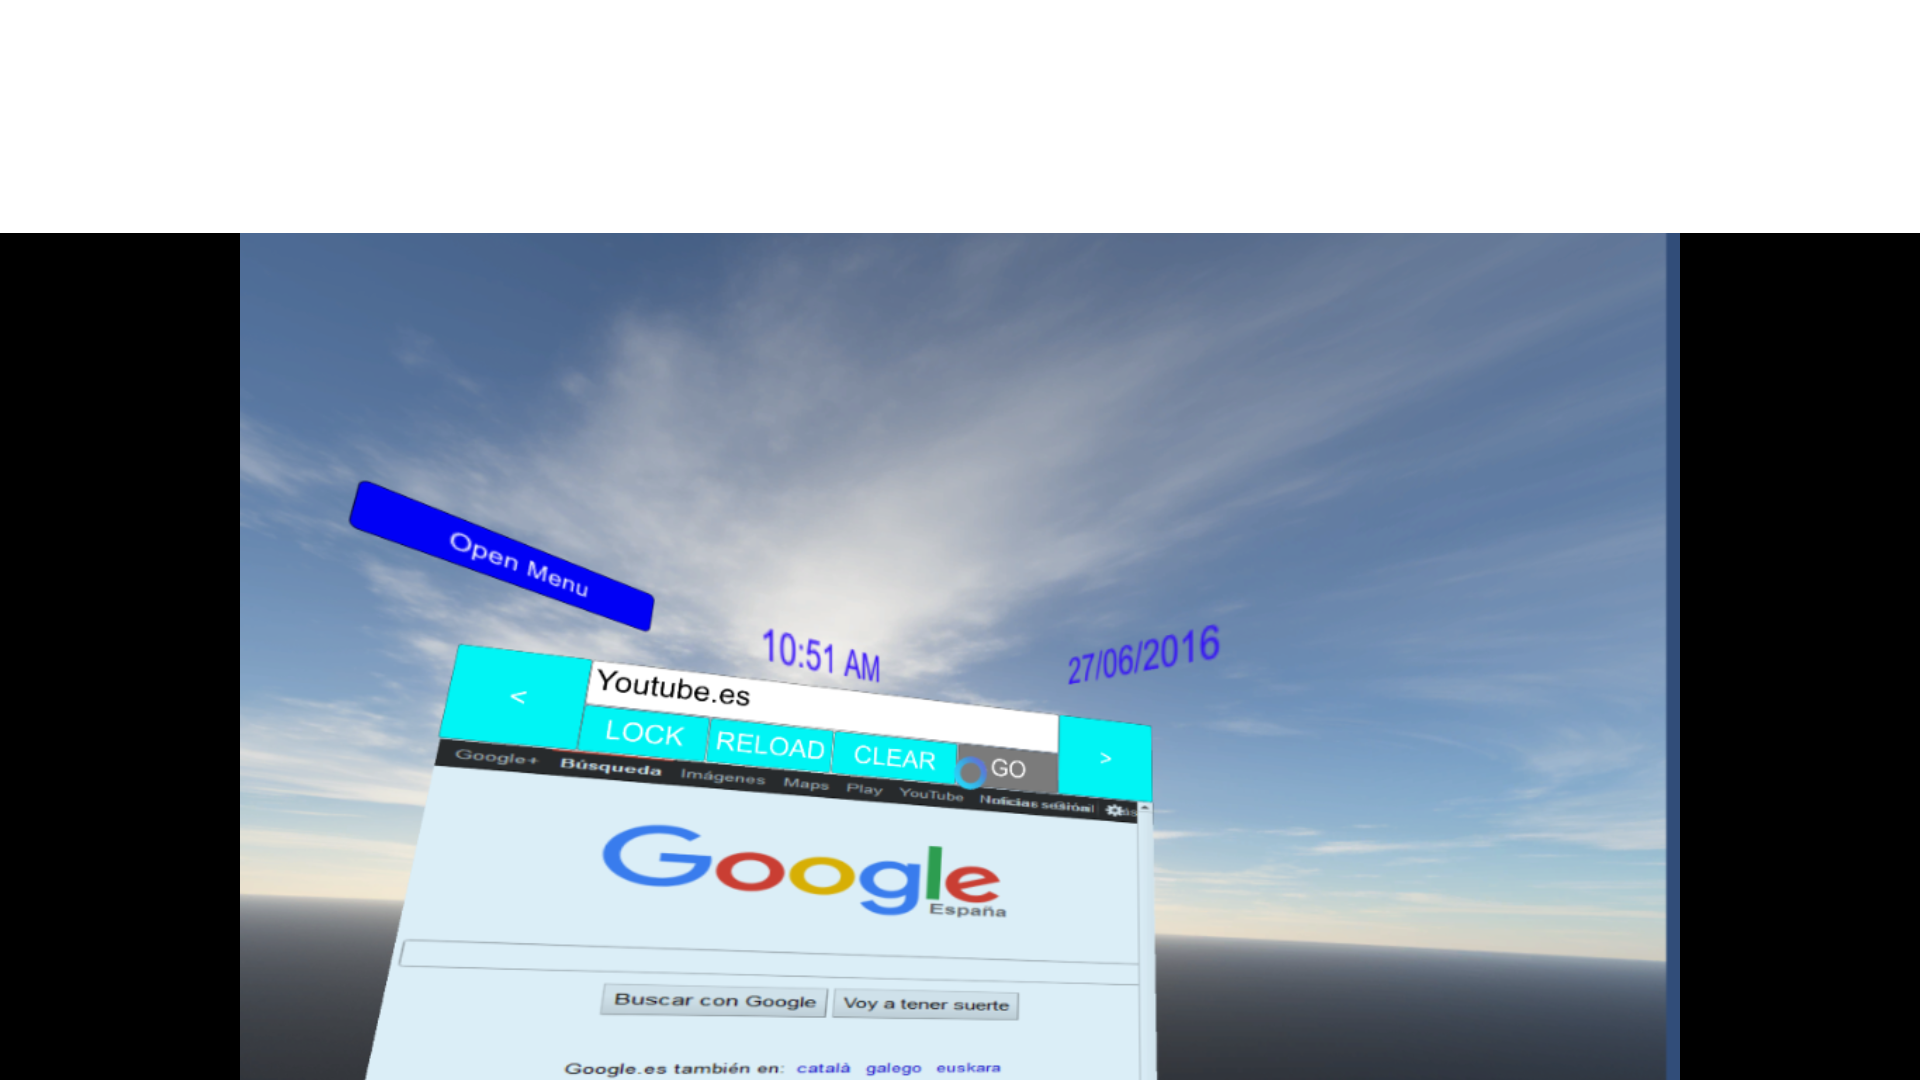
\includegraphics[width=\textwidth]{images/carga_url.png} 
  \caption{Cargando la URL.}
  \label{fig:loadURL}
\end{figure}

\begin{figure} [H]
\centering	
	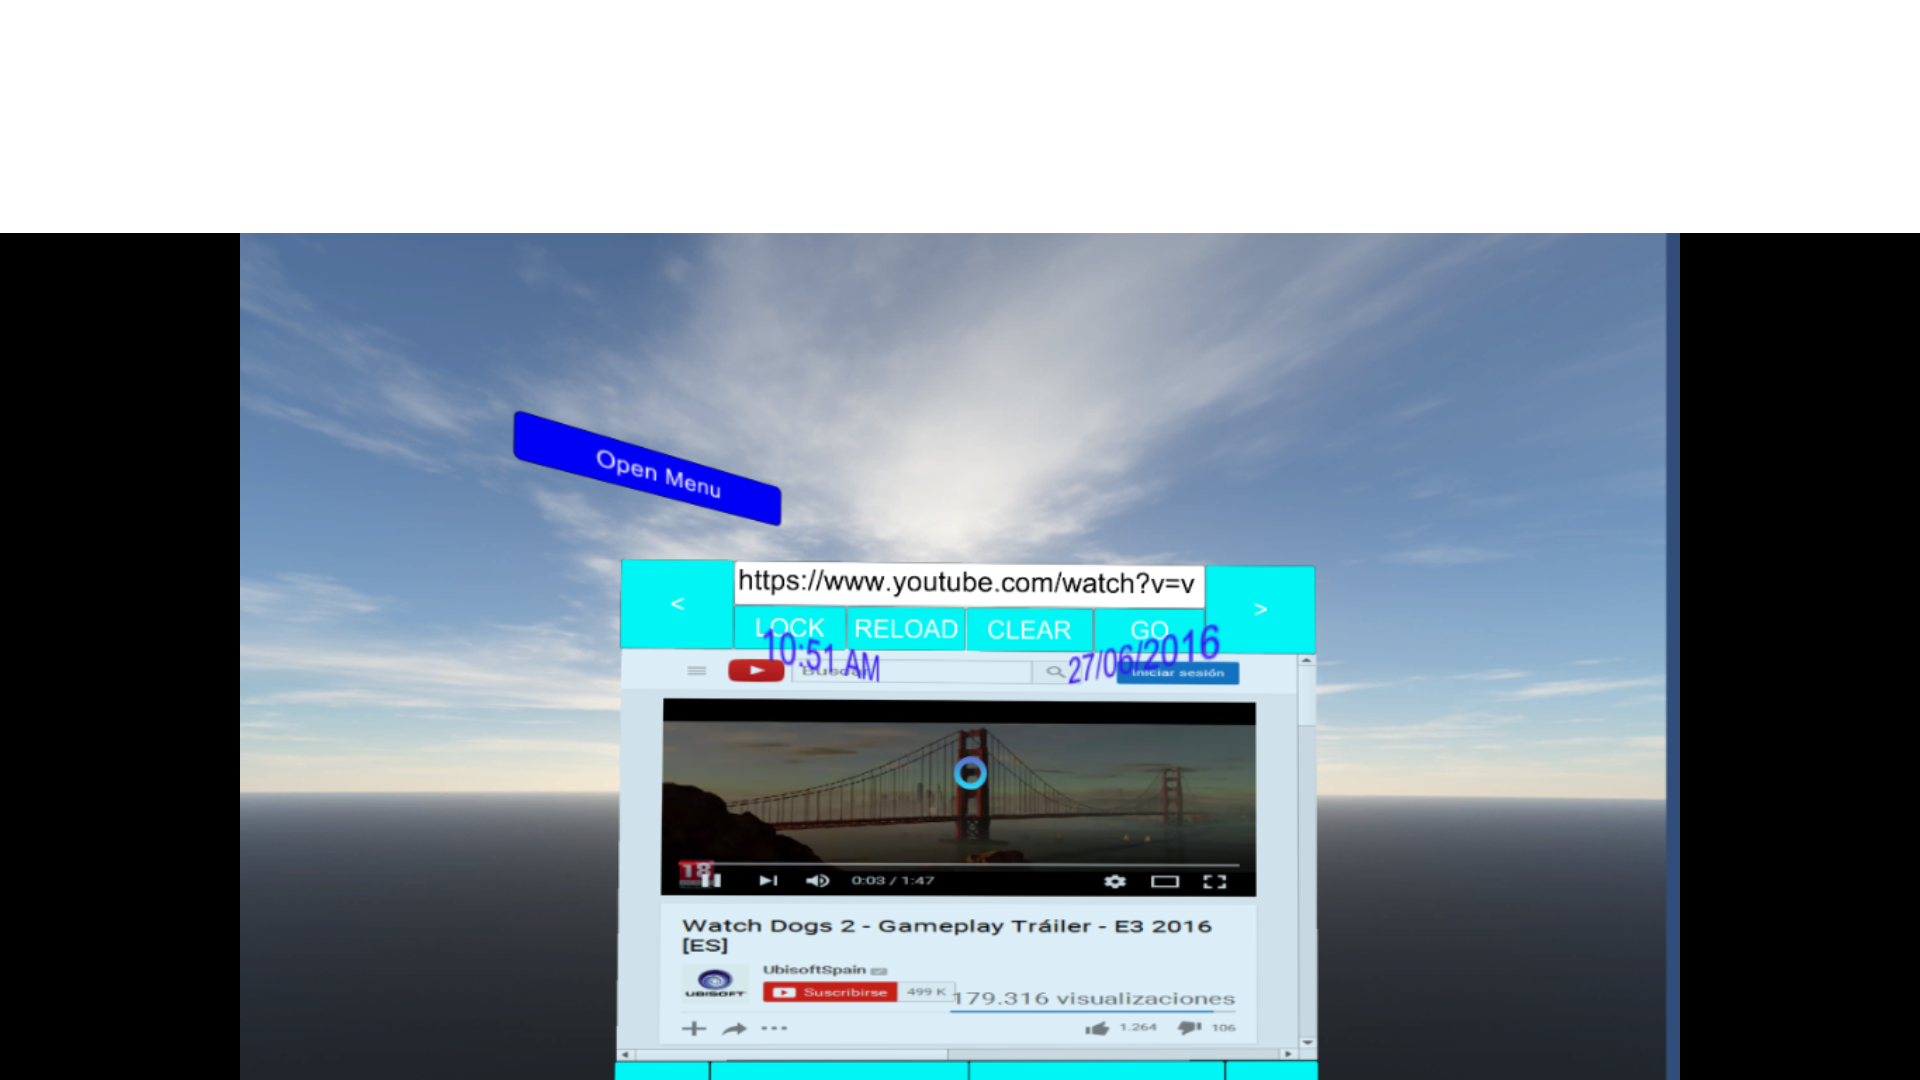
\includegraphics[width=\textwidth]{images/video.png} 
  \caption{Visualizando un v�deo.}
  \label{fig:browser2}
\end{figure}

\begin{figure} [H]
\centering	
	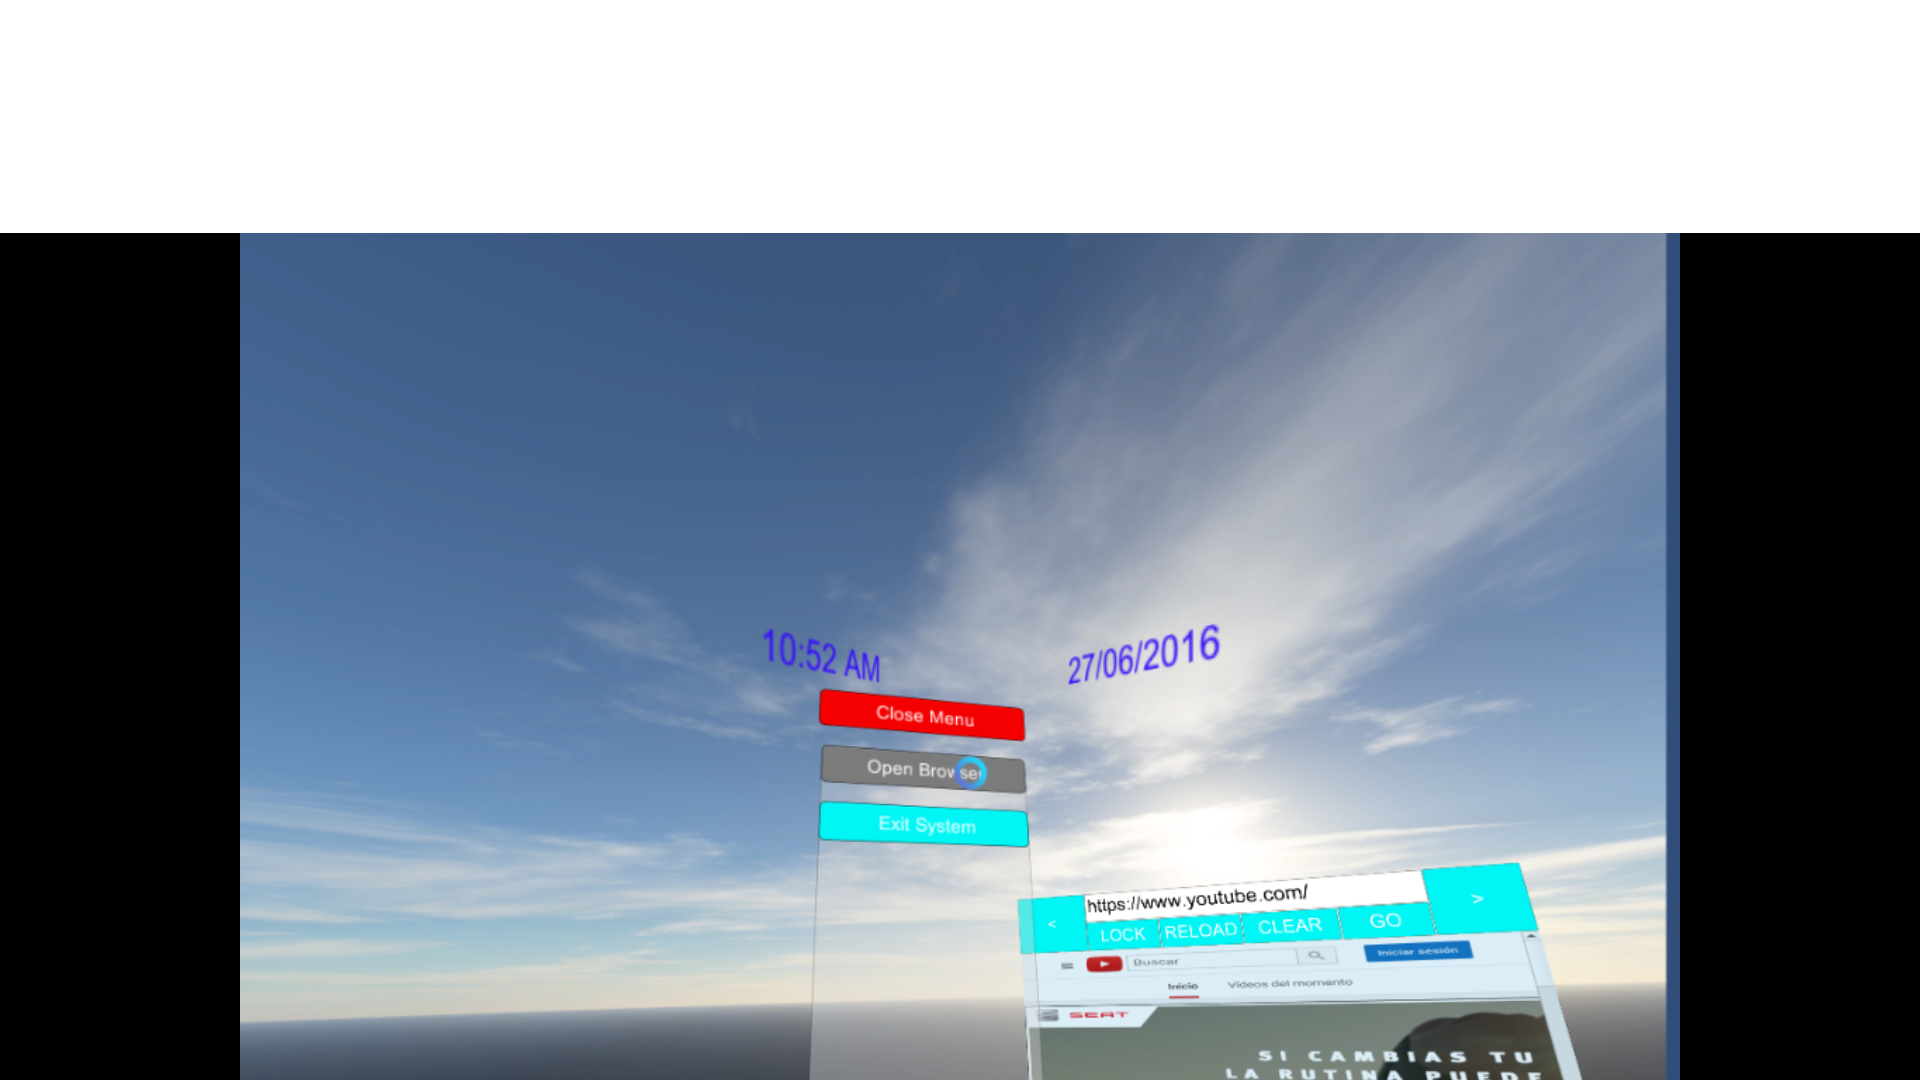
\includegraphics[width=\textwidth]{images/cierre_navegador.png} 
  \caption{Usuario seleccionado la opci�n para cerrar el navegador.}
  \label{fig:exitBrowser2}
\end{figure}

\begin{figure} [H]
\centering	
	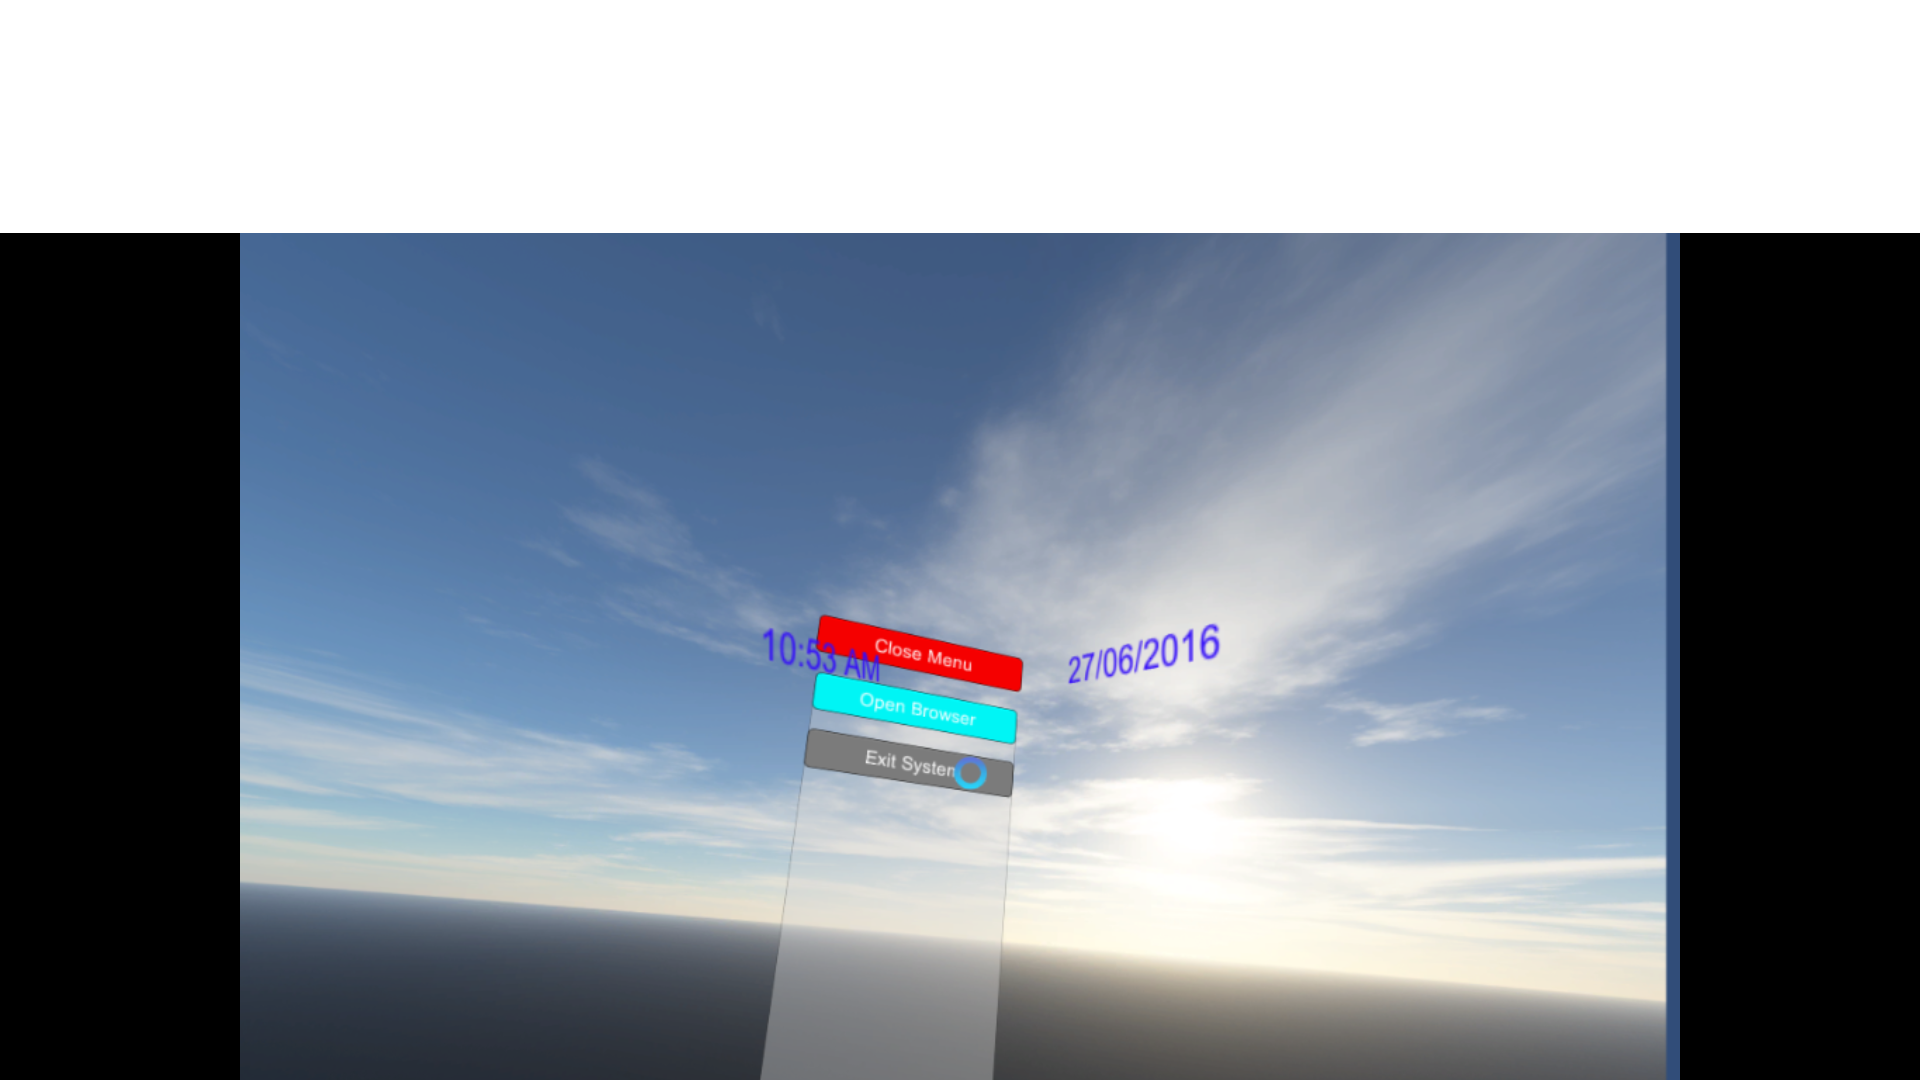
\includegraphics[width=\textwidth]{images/salir_sistema.png} 
  \caption{Usuario seleccionado la opci�n para apagar el sistema}
  \label{fig:exit3}
\end{figure}

\newpage \thispagestyle{empty} % P�gina vac�a 


\chapter{C�digo Fuente}
\label{Anexo:codigo}

En este anexo va incluido el c�digo fuente del desarrollo de este TFG. La codificaci�n no es lo principal en este software sino que hay detr�s un trabajo de dise�o 3D que encaja con todo este c�digo. Se adjunta la URL desde la que se puede descargar todo el c�digo y el proyecto de \emph{Unity 3D}: \url{https://www.dropbox.com/s/h7nz0ny43y9weu7/TFG_Cristian_Fernandez_Del_Pozo_v1_2016_Source.rar?dl=0}

Los cuadros de c�digo reciben la nomenclatura de Listing.

\lsection{Menu}
En esta secci�n se incluyen los c�digos que dan funcionalidad al men� de la aplicaci�n.

El c�digo descrito en Listing \ref{menuTrigger} abre y cierra el men�.
\begin{lstlisting}[label=menuTrigger,caption=MenuTrigger]
using UnityEngine;
using System.Collections;
using UnityEngine.UI;

public class MenuTrigger : MonoBehaviour {

	[Header("Trigger Click Button")]
	public Button TriggerButton;

	[Header("MenuPanel")]
	public GameObject Panel;

	private ColorBlock colorOn;
	private ColorBlock colorOff;

	void Start (){
	
		colorOn = new ColorBlock ();
		colorOn.normalColor = Color.red;
		colorOn.highlightedColor = Color.gray;
		colorOn.colorMultiplier = 1;

		colorOff = new ColorBlock ();
		colorOff.normalColor = Color.blue;
		colorOff.highlightedColor = Color.gray;
		colorOff.colorMultiplier = 1;
	}

	public void OnClickEvent(){
		Debug.Log ("Click!");

		if(Panel.GetComponent<Animator>().GetBool("isVisible")){
			Debug.Log("Ocultate!");		

			var results = Panel.GetComponentsInChildren<Button>(true);
			Panel.GetComponent<Animator>().SetBool("isVisible",false);
			Panel.GetComponent<Animator>().SetTrigger("PlayClose");

			foreach(Button button in results){
				button.gameObject.SetActive(false);
			}

			if (TriggerButton != null) {
				TriggerButton.colors = colorOff;
				TriggerButton.GetComponentInChildren<Text> ().text = "Open Menu";
			}



		}else{
			Debug.Log("Muestrate!!");

			Panel.GetComponent<Animator>().SetBool("isVisible",true);
			Panel.GetComponent<Animator>().SetTrigger("PlayOpen");
			var results = Panel.GetComponentsInChildren<Button>(true);

			if (TriggerButton != null) {
				TriggerButton.colors = colorOn;
				TriggerButton.GetComponentInChildren<Text> ().text = "Close Menu";
			}

			
			foreach(Button button in results){
				button.gameObject.SetActive(true);
			}
		}
	}
}


\end{lstlisting}
\newpage
El c�digo descrito en Listing \ref{browserTrigger} abre y cierra el navegador.
\begin{lstlisting}[label=browserTrigger,caption=BrowserTrigger]
using UnityEngine;
using System.Collections;
using UnityEngine.UI;

public class BrowserTrigger : MonoBehaviour {

	[Header("TriggerButton")]
	public Button TriggerButton;

	public void OnClickEvent(){

		ColorBlock colorOn = new ColorBlock ();
		colorOn.normalColor = Color.red;
		colorOn.highlightedColor = Color.gray;
		colorOn.colorMultiplier = 1;

		ColorBlock colorOff = new ColorBlock ();
		colorOff.normalColor = Color.cyan;
		colorOff.highlightedColor = Color.gray;
		colorOff.colorMultiplier = 1;

		Debug.Log ("Click!");

		if(gameObject.GetComponent<Animator>().GetBool("isVisible")){
			Debug.Log("Ocultate!");		

			if (TriggerButton != null) {
				TriggerButton.colors = colorOff;
				TriggerButton.GetComponentInChildren<Text> ().text = "Open Browser";
			}

			gameObject.GetComponent<Animator>().SetBool("isVisible",false);
			gameObject.GetComponent<Animator>().SetTrigger("CloseBrowser");

//			var results = gameObject.GetComponentsInChildren<GameObject>(true);
//			foreach(GameObject button in results){
//				button.SetActive(false);
//			}
//

		}else{
			Debug.Log("Muestrate!!");

			if (TriggerButton != null) {
				TriggerButton.colors = colorOn;
				TriggerButton.GetComponentInChildren<Text> ().text = "Close Browser";
			}

			gameObject.GetComponent<Animator>().SetBool("isVisible",true);
			gameObject.GetComponent<Animator>().SetTrigger("OpenBrowser");
//			var results = gameObject.GetComponentsInChildren<GameObject>(true);
//
//
//			foreach(GameObject button in results){
//				button.SetActive(true);
//			}
		}
	}
}

\end{lstlisting}


El c�digo descrito en Listing \ref{Quit} apaga el sistema entero.
\begin{lstlisting}[label=Quit,caption=Quit]
using UnityEngine;
using System.Collections;

public class Quit : MonoBehaviour {

	public void OnClickEvent(){
		Application.Quit ();
	}
}
\end{lstlisting}

\lsection{Panel de informaci�n}

En esta secci�n se muestra el c�digo que establece la fecha y la hora del sistema en el panel de informaci�n. Listing \ref{info}
\begin{lstlisting}[label=info,caption=InfoPanelController]
#pragma strict

var dateText:UI.Text;
var timeText:UI.Text;


function Start () {

}

function Update () {


	dateText.text = System.DateTime.Now.ToString("dd/MM/yyyy");
	timeText.text = System.DateTime.Now.ToShortTimeString();
	

}
\end{lstlisting}

\lsection{Navegador}
En esta secci�n se describe el c�digo necesario para la interacci�n con el navegador. 

El Listing \ref{webViewer} muestra la adaptaci�n del c�digo proporcionado por \emph{uWebKit}.

\begin{lstlisting}[label=webViewer,caption=webTexture]
/******************************************
  * uWebKit 
  * (c) 2014 THUNDERBEAST GAMES, LLC
  * http://www.uwebkit.com
  * sales@uwebkit.com
*******************************************/

/******************************************
	* Mod by Cristian Fern�ndez for TFG proyect 
	* Under University License
	* cristian.fernandez@estudiante.uam.es
	* 2016
*******************************************/

using UnityEngine;
using System.Collections;
using System.Collections.Generic;
using UnityEngine.EventSystems;
using UnityEngine.UI;

/// <summary>
/// Basic example of using a UWKWebView on a 3D Unity surface
/// </summary>
 
// IMPORTANT: Please see the WebGUI.cs example for 2D support

public class WebTexture : MonoBehaviour,IPointerExitHandler,IPointerEnterHandler
{
    
	#region Inspector Fields

	[Header ("Buttons")]
	public Button BlockedClicksText;

	[Header ("InputFields")]
	public InputField URLInput;

	[Header ("CrossHair Animator")]
	public Animator CrossHairAnimator;

	[Header ("Web Options")]
	public bool KeyboardEnabled = true;
	public bool MouseEnabled = true;
	public bool Rotate = false;
	public bool HasFocus = true;
	public bool AlphaMask = false;

	#endregion

	private bool _isInIt = false;

	private Vector3 _previousMousePosition = Vector3.zero;
	private Vector3 _previous2MousePosition = Vector3.zero;
	private Vector3 _previous3MousePosition = Vector3.zero;

	private bool _isBlocked = false;

	private bool _hasClicked = false;

	UWKWebView view;

	Camera _camera = null;
	private int _counter = 0;
	private int _ClickCounter = 0;
	private int _X =0;
	private int _Y = 0;
	private int _posX = 0;
	private int _posY = 0;


	// Use this for initialization
	void Start ()
	{   
		
		view = gameObject.GetComponent<UWKWebView> ();

		_camera = Camera.main;

		view.SetAlphaMask (AlphaMask);
		view.SetFrameRate (60);

		if (URLInput != null) {
			URLInput.text = view.URL;

			view.URLChanged = new URLChangedDelegate ((v,url)=>{

				URLInput.text = url;

			});

		}


#if !UNITY_4_6
		if (GetComponent<Renderer> () != null)
			GetComponent<Renderer> ().material.mainTexture = view.WebTexture;

		if (GetComponent<GUITexture> () != null)
			GetComponent<GUITexture> ().texture = view.WebTexture;
#else
        if (renderer != null)
            renderer.material.mainTexture = view.WebTexture;

        if (guiTexture != null)
            guiTexture.texture = view.WebTexture;
#endif         

		Cursor.lockState = CursorLockMode.Locked;
		_counter = 0;
		_ClickCounter = 0;
	}
    
	// Update is called once per frame
	void Update ()
	{
                                        
		if (Rotate)
			gameObject.transform.Rotate (0, Time.deltaTime * 4.0f, 0);

		if (!HasFocus || !_isInIt)
			return;         
		double tolx = view.CurrentWidth * 0.02;
		double toly = view.CurrentHeight * 0.02;
		RaycastHit rcast;

		Ray r2 = _camera.ScreenPointToRay (Input.mousePosition);
		Debug.DrawRay (r2.origin, r2.direction, Color.red);

		if (_counter % 61 == 0) {

			_counter = 0;

			if (Physics.Raycast (r2, out rcast)) {
				if (rcast.collider != GetComponent<MeshCollider> ()) {
					return;
				}

				int x = (int)(rcast.textureCoord.x * (float)view.MaxWidth);
				int y = view.MaxHeight - (int)(rcast.textureCoord.y * (float)view.MaxHeight);

				Vector3 mousePos = new Vector3 ();
				mousePos.x = x; 
				mousePos.y = y;

				view.ProcessMouse (mousePos);

				if (!Utils.Compare2Vector3WithTolerance (_previousMousePosition, mousePos, tolx, toly)) {

					if (_ClickCounter < 50) {
						_ClickCounter++;
					} else {
						_ClickCounter = 0;
						if (!_isBlocked && !_hasClicked) {
							_hasClicked = true;
							CrossHairAnimator.SetTrigger ("Play");
							MouseOperations.MouseEvent (MouseOperations.MouseEventFlags.LeftUp | MouseOperations.MouseEventFlags.LeftDown);
							Debug.Log ("Click WEBVIEW");
						} else {
							_hasClicked = false;
						}
					}

				}

				_previousMousePosition = mousePos;
			}
		
		} else {
			_counter++;
		}
	}

	public void LoadURL(){

		if (view != null && URLInput != null) {

			string url = Utils.CheckURL (URLInput.text);

			view.LoadURL (url);


		
		}

	
	}

	public void ScrollUP(){
		if (view != null && _Y != 0) {
			_Y -= 1;
			_posY = (int)(_Y * (view.ContentHeight * 0.05));
			view.SetScrollPosition (_posX, _posY);
		}
	}

	public void ScrollDown(){
		if (view != null) {

			_Y +=1;

			_posY = (int)(_Y * (view.ContentHeight * 0.05));


			view.SetScrollPosition (_posX, _posY);
		}
	}

	public void ScrollLeft(){
		if (view != null && _X != 0) {
			_X -= 1;
			_posX = (int)(_Y * (view.ContentWidth * 0.05));
			view.SetScrollPosition (_posX, _posY);
		}
	}

	public void ScrollRight(){
		if (view != null) {

			_X +=1;

			_posX = (int)(_X * (view.ContentWidth * 0.05));


			view.SetScrollPosition (_posX, _posY);
		}
	}
        
	void OnGUI ()
	{       
		if (!KeyboardEnabled || !HasFocus)
			return;
        
		if (Event.current.isKey) {
			view.ProcessKeyboard (Event.current);
		}
        
	}

	#region IPointerEnterHandler implementation

	public void OnPointerEnter (PointerEventData eventData)
	{
		_isInIt = true;
		_hasClicked = false;

	}

	#endregion




	#region IPointerExitHandler implementation

	public void OnPointerExit (PointerEventData eventData)
	{
		_isInIt = false;
		_hasClicked = false;
	}

	#endregion

	public void OnBlockedEvent ()
	{
		_isBlocked = !_isBlocked;

		ColorBlock color = new ColorBlock ();

		if (_isBlocked) {
			BlockedClicksText.GetComponentInChildren<Text> ().text = "UNLOCK";
			color.normalColor = Color.red;
			color.highlightedColor = Color.gray;
		} else {
			BlockedClicksText.GetComponentInChildren<Text> ().text = "LOCK";
			color.normalColor = Color.cyan;
			color.highlightedColor = Color.gray;
		}
		color.colorMultiplier = 1;
		BlockedClicksText.colors = color;

	}

}

\end{lstlisting}

El c�digo mostrado en el Listing \ref{urlController} corresponde a las funcionalidades del teclado y el campo de introducci�n de la URL.

\begin{lstlisting}[label=urlController,caption=urlController]
using UnityEngine;
using System.Collections;
using UnityEngine.UI;

public class URLController : MonoBehaviour {

	private InputField _input;

	// Use this for initialization
	void Start () {
		_input = GetComponent<InputField> ();
	}
	
	// Update is called once per frame
	void Update () {

	}

	public void Clear(){
		_input.text = "";
	}

	void OnGUI()
	{
		if (_input.isFocused) {

			Event e = Event.current;

			if (Input.anyKeyDown && e.isKey) {
				Debug.Log ("Detected key code: " + e.keyCode);
				if (_input != null && e.keyCode != KeyCode.None) {
					if (e.keyCode == KeyCode.Backspace) {
						_input.text = _input.text.Substring (0, _input.text.Length - 1); 
					} else if (e.keyCode == KeyCode.Period) {
						_input.text += ".";
					} else if (e.keyCode == KeyCode.BackQuote) {
						_input.text += "�";
					}else if (e.keyCode == KeyCode.KeypadDivide) {
						_input.text += "/";
					} else {
						_input.text += e.keyCode.ToString ().ToLower ();		
					}
					 	
				}

			}
		}

	}
}


\end{lstlisting}

\lsection{Teclado Virtual}
El c�digo mostrado en esta secci�n corresponde a las funcionalidades propias del teclado virtual de la aplicaci�n. Listing \ref{vk}.

\begin{lstlisting}[label=vk,caption=Virtual KeyboardController]
using System;
using UnityEngine;
using UnityEngine.UI;
using WindowsInput;

public class KeyboardController : MonoBehaviour
{
	[Header("Input Text")]
	public InputField Input;

	[Header("Controller Button")]
	public Button ClearController;
	public Button GoController;

	[Header("Letter Buttons")]
	public Button A;
	public Button B;
	public Button C;
	public Button D;
	public Button E;
	public Button F;
	public Button G;
	public Button H;
	public Button I;
	public Button J;
	public Button K;
	public Button L;
	public Button M;
	public Button N;
	public Button �;
	public Button O;
	public Button P;
	public Button Q;
	public Button R;
	public Button S;
	public Button T;
	public Button U;
	public Button V;
	public Button W;
	public Button X;
	public Button Y;
	public Button Z;

	[Header("Number Buttons")]
	public Button B1;
	public Button B2;
	public Button B3;
	public Button B4;
	public Button B5;
	public Button B6;
	public Button B7;
	public Button B8;
	public Button B9;
	public Button B0;

	[Header("Simbol Buttons")]
	public Button Dot;
	public Button Comma;
	public Button Guion;

	[Header("Command Buttons")]
	public Button Mayus;
	public Button Ret;
	public Button Enter;
	public Button Space;

	private bool _urlWrite = false;

	void Start ()
	{
		if (ClearController != null) {
			ClearController.onClick.AddListener (() => {
				_urlWrite = true;
			});
		}

		if (GoController != null) {
			GoController.onClick.AddListener(()=>{
				_urlWrite = false;
			});
		}

		if (A != null) {
			A.onClick.AddListener (() => {

				if(Input != null&& _urlWrite){
					Input.text+="a";
				}else{
					KeyBoardOperation.PressKey(VirtualKeyCode.VK_A);

				}

			});

		}



		if (B != null) {
			B.onClick.AddListener (() => {

				if(Input != null&& _urlWrite){
					Input.text+="b";
				}else{
					KeyBoardOperation.PressKey(VirtualKeyCode.VK_B);

				}
			});
		}

		if (C != null) {
			C.onClick.AddListener (() => {

				if(Input != null&& _urlWrite){
					Input.text+="c";
				}else{
					KeyBoardOperation.PressKey(VirtualKeyCode.VK_C);

				}
			});
		}

		if (D != null) {
			D.onClick.AddListener (() => {

				if(Input != null&& _urlWrite){
					Input.text+="d";
				}else{
					KeyBoardOperation.PressKey(VirtualKeyCode.VK_D);

				}

			});
		}

		if (E != null) {
			E.onClick.AddListener (() => {

				if(Input != null&& _urlWrite){
					Input.text+="e";
				}else{
					KeyBoardOperation.PressKey(VirtualKeyCode.VK_E);

				}
			});
		}

		if (F != null) {
			F.onClick.AddListener (() => {

				if(Input != null&& _urlWrite){
					Input.text+="f";
				}else{
					KeyBoardOperation.PressKey(VirtualKeyCode.VK_F);

				}
			});
		}

		if (G != null) {
			G.onClick.AddListener (() => {

				if(Input != null&& _urlWrite){
					Input.text+="g";
				}else{
					KeyBoardOperation.PressKey(VirtualKeyCode.VK_G);
				}
			});
		}

		if (H != null) {
			H.onClick.AddListener (() => {

				if(Input != null&& _urlWrite){
					Input.text+="h";
				}else{
					KeyBoardOperation.PressKey(VirtualKeyCode.VK_H);
				}
			});
		}

		if (I != null) {
			I.onClick.AddListener (() => {

				if(Input != null&& _urlWrite){
					Input.text+="i";
				}else{
					KeyBoardOperation.PressKey(VirtualKeyCode.VK_I);
				}

			});
		}

		if (J != null) {
			J.onClick.AddListener (() => {

				if(Input != null&& _urlWrite){
					Input.text+="J";
				}else{
					KeyBoardOperation.PressKey(VirtualKeyCode.VK_J);
				}
			});
		}

		if (K != null) {
			K.onClick.AddListener (() => {

				if(Input != null&& _urlWrite){
					Input.text+="K";
				}else{
					KeyBoardOperation.PressKey(VirtualKeyCode.VK_K);
				}

			});
		}

		if (L != null) {
			L.onClick.AddListener (() => {

				if(Input != null&& _urlWrite){
					Input.text+="l";
				}else{
					KeyBoardOperation.PressKey(VirtualKeyCode.VK_L);
				}
			});
		}

		if (M != null) {
			M.onClick.AddListener (() => {

				if(Input != null&& _urlWrite){
					Input.text+="m";
				}else{
					KeyBoardOperation.PressKey(VirtualKeyCode.VK_M);
				}

			});
		}

		if (N != null) {
			N.onClick.AddListener (() => {

				if(Input != null&& _urlWrite){
					Input.text+="n";
				}else{
					KeyBoardOperation.PressKey(VirtualKeyCode.VK_N);
				}

			});
		}

		if (� != null) {
			�.onClick.AddListener (() => {

				if(Input != null&& _urlWrite){
					Input.text+="�";
				}else{
					KeyBoardOperation.PressSpecialKey("�");
				}

			});
		}

		if (O != null) {
			O.onClick.AddListener (() => {

				if(Input != null&& _urlWrite){
					Input.text+="o";
				}else{
					KeyBoardOperation.PressKey(VirtualKeyCode.VK_O);
				}

			});
		}

		if (P != null) {
			P.onClick.AddListener (() => {

				if(Input != null&& _urlWrite){
					Input.text+="p";
				}else{
					KeyBoardOperation.PressKey(VirtualKeyCode.VK_P);
				}

			});
		}

		if (Q != null) {
			Q.onClick.AddListener (() => {

				if(Input != null&& _urlWrite){
					Input.text+="q";
				}else{
					KeyBoardOperation.PressKey(VirtualKeyCode.VK_Q);
				}

			});
		}

		if (R != null) {
			R.onClick.AddListener (() => {

				if(Input != null&& _urlWrite){
					Input.text+="r";
				}else{
					KeyBoardOperation.PressKey(VirtualKeyCode.VK_R);
				}

			});
		}

		if (S != null) {
			S.onClick.AddListener (() => {

				if(Input != null&& _urlWrite){
					Input.text+="s";
				}else{
					KeyBoardOperation.PressKey(VirtualKeyCode.VK_S);
				}

			});
		}

		if (T != null) {
			T.onClick.AddListener (() => {

				if(Input != null&& _urlWrite){
					Input.text+="t";
				}else{
					KeyBoardOperation.PressKey(VirtualKeyCode.VK_T);
				}

			});
		}

		if (U != null) {
			U.onClick.AddListener (() => {

				if(Input != null&& _urlWrite){
					Input.text+="u";
				}else{
					KeyBoardOperation.PressKey(VirtualKeyCode.VK_U);
				}

			});
		}

		if (V != null) {
			V.onClick.AddListener (() => {

				if(Input != null&& _urlWrite){
					Input.text+="v";
				}else{
					KeyBoardOperation.PressKey(VirtualKeyCode.VK_V);

				}

			});
		}


		if (W != null) {
			W.onClick.AddListener (() => {

				if(Input != null&& _urlWrite){
					Input.text+="w";
				}else{
					KeyBoardOperation.PressKey(VirtualKeyCode.VK_W);

				}

			});
		}

		if (X != null) {
			X.onClick.AddListener (() => {

				if(Input != null&& _urlWrite){
					Input.text+="x";
				}else{
					KeyBoardOperation.PressKey(VirtualKeyCode.VK_X);

				}

			});
		}

		if (Y != null) {
			Y.onClick.AddListener (() => {
				

				if(Input != null&& _urlWrite){
					Input.text+="Y";
				}else{
					KeyBoardOperation.PressKey(VirtualKeyCode.VK_Y);
				}

			});
		}

		if (Z != null) {
			Z.onClick.AddListener (() => {
				

				if(Input != null&& _urlWrite){
					Input.text+="z";
				}else{
					KeyBoardOperation.PressKey(VirtualKeyCode.VK_Z);
				}

			});
		}

		if (B0 != null) {
			B0.onClick.AddListener (() => {


				if(Input != null&& _urlWrite){
					Input.text+="0";
				}else{
					KeyBoardOperation.PressKey(VirtualKeyCode.VK_0);
				}

			});
		}

		if (B1 != null) {
			B1.onClick.AddListener (() => {


				if(Input != null&& _urlWrite){
					Input.text+="1";
				}else{
					KeyBoardOperation.PressKey(VirtualKeyCode.VK_1);
				}

			});
		}

		if (B2 != null) {
			B2.onClick.AddListener (() => {


				if(Input != null&& _urlWrite){
					Input.text+="2";
				}else{
					KeyBoardOperation.PressKey(VirtualKeyCode.VK_2);
				}

			});
		}
		if (B3 != null) {
			B3.onClick.AddListener (() => {


				if(Input != null&& _urlWrite){
					Input.text+="3";
				}else{
					KeyBoardOperation.PressKey(VirtualKeyCode.VK_3);
				}

			});
		}

		if (B4 != null) {
			B4.onClick.AddListener (() => {


				if(Input != null&& _urlWrite){
					Input.text+="4";
				}else{
					KeyBoardOperation.PressKey(VirtualKeyCode.VK_4);
				}

			});
		}

		if (B5 != null) {
			B5.onClick.AddListener (() => {


				if(Input != null&& _urlWrite){
					Input.text+="5";
				}else{
					KeyBoardOperation.PressKey(VirtualKeyCode.VK_5);
				}

			});
		}

		if (B6 != null) {
			B6.onClick.AddListener (() => {


				if(Input != null&& _urlWrite){
					Input.text+="6";
				}else{
					KeyBoardOperation.PressKey(VirtualKeyCode.VK_6);
				}

			});
		}

		if (B7 != null) {
			B7.onClick.AddListener (() => {


				if(Input != null&& _urlWrite){
					Input.text+="7";
				}else{
					KeyBoardOperation.PressKey(VirtualKeyCode.VK_7);
				}

			});
		}

		if (B8 != null) {
			B8.onClick.AddListener (() => {


				if(Input != null&& _urlWrite){
					Input.text+="8";
				}else{
					KeyBoardOperation.PressKey(VirtualKeyCode.VK_8);
				}

			});
		}
		if (B9 != null) {
			B9.onClick.AddListener (() => {


				if(Input != null&& _urlWrite){
					Input.text+="9";
				}else{
					KeyBoardOperation.PressKey(VirtualKeyCode.VK_9);
				}

			});
		}

		if (Dot != null) {
			Dot.onClick.AddListener (() => {


				if(Input != null&& _urlWrite){
					Input.text+=".";
				}else{
					KeyBoardOperation.PressSpecialKey(".");
				}

			});
		}

		if (Comma != null) {
			Comma.onClick.AddListener (() => {


				if(Input != null&& _urlWrite){
					Input.text+=",";
				}else{
					KeyBoardOperation.PressSpecialKey(",");
				}

			});
		}

		if (Guion != null) {
			Guion.onClick.AddListener (() => {


				if(Input != null&& _urlWrite){
					Input.text+="-";
				}else{
					KeyBoardOperation.PressSpecialKey("-");
				}

			});
		}

		if (Enter != null) {
			Enter.onClick.AddListener (() => {

				KeyBoardOperation.PressKey(VirtualKeyCode.RETURN);


			});
		}

		if (Ret != null) {
			Ret.onClick.AddListener (() => {
				if(Input != null&& _urlWrite){
					Input.text =Input.text.Substring(0,Input.text.Length-1);
				}else{
					KeyBoardOperation.PressKey(VirtualKeyCode.BACK);
				}


			});
		}


		if (Space != null) {
			Space.onClick.AddListener (() => {

				KeyBoardOperation.PressKey(VirtualKeyCode.SPACE);

			});
		}

		if (Mayus != null) {

			ColorBlock colorOn = new ColorBlock ();
			colorOn.normalColor = Color.red;
			colorOn.highlightedColor = Color.gray;
			colorOn.colorMultiplier = 1;

			ColorBlock colorOff = new ColorBlock ();
			colorOff.normalColor = Color.blue;
			colorOff.highlightedColor = Color.gray;
			colorOff.colorMultiplier = 1;

			Mayus.colors = (KeyBoardOperation.IsCapitalLetter()) ? colorOn : colorOff;
			
			Mayus.onClick.AddListener (() => {

				var prev = KeyBoardOperation.IsCapitalLetter();
				prev =!prev;

				KeyBoardOperation.PressKey(VirtualKeyCode.CAPITAL);

				Mayus.colors = (prev) ? colorOn : colorOff;

			});
		}


	}

}
\end{lstlisting}

\lsection{Sistema de interacci�n Gaze}

En esta secci�n se muestra el c�digo necesario para adaptar el sistema Gaze Input al trabajo realizado. Listing \ref{inputGaze}.
\begin{lstlisting}[label=inputGaze,caption=GazeInput]
// Gaze Input Module by Peter Koch <peterept@gmail.com>

/******************************************
	* Mod by Cristian Fern�ndez for TFG proyect 
	* Under University License
	* cristian.fernandez@estudiante.uam.es
	* 2016
*******************************************/

using UnityEngine;
using UnityEngine.EventSystems;
using System.Collections.Generic;

// To use:
// 1. Drag onto your EventSystem game object.
// 2. Disable any other Input Modules (eg: StandaloneInputModule & TouchInputModule) as they will fight over selections.
// 3. Make sure your Canvas is in world space and has a GraphicRaycaster (should by default).
// 4. If you have multiple cameras then make sure to drag your VR (center eye) camera into the canvas.
public class GazeInputModule : PointerInputModule 
{
	public enum Mode { Click = 0, Gaze };
	public Mode mode;

	[Header("Click Settings")]
	public string ClickInputName = "Submit";
	[Header("Gaze Settings")]
	public float GazeTimeInSeconds = 2f;

	[Header("CrossHair Animator")]
	public Animator CrossHairAnimator;

	public RaycastResult CurrentRaycast;

	private PointerEventData pointerEventData;
	private GameObject currentLookAtHandler;
	private float currentLookAtHandlerClickTime;

	public override void Process()
	{ 
		HandleLook();
		HandleSelection();
	}

	void HandleLook()
	{
		if (pointerEventData == null)
		{
			pointerEventData = new PointerEventData(eventSystem);
		}
		// fake a pointer always being at the center of the screen
		pointerEventData.position = new Vector2(Screen.width/2, Screen.height/2);
		pointerEventData.delta = Vector2.zero;
		List<RaycastResult> raycastResults = new List<RaycastResult>();
		eventSystem.RaycastAll(pointerEventData, raycastResults);
		CurrentRaycast = pointerEventData.pointerCurrentRaycast = FindFirstRaycast(raycastResults);
		ProcessMove(pointerEventData);
	}
	
	void HandleSelection()
	{
		if (pointerEventData.pointerEnter != null)
		{

			// if the ui receiver has changed, reset the gaze delay timer 
			GameObject handler = ExecuteEvents.GetEventHandler<IPointerClickHandler>(pointerEventData.pointerEnter);
			if (currentLookAtHandler != handler)
			{
				currentLookAtHandler = handler;

				currentLookAtHandlerClickTime = Time.realtimeSinceStartup + GazeTimeInSeconds;
				
				CrossHairAnimator.SetTrigger("Play");

			}
			// if we have a handler and it's time to click, do it now
			if (currentLookAtHandler != null && 
			    (mode == Mode.Gaze && Time.realtimeSinceStartup > currentLookAtHandlerClickTime) || 
			    (mode == Mode.Click && Input.GetButtonDown(ClickInputName)))
			{
				if (EventSystem.current.currentSelectedGameObject != null)
				{
					Debug.Log ("old" + EventSystem.current.currentSelectedGameObject.name);
					GameObject currentSelected  = EventSystem.current.currentSelectedGameObject;

		//			ExecuteEvents.ExecuteHierarchy(EventSystem.current.currentSelectedGameObject, pointerEventData, ExecuteEvents.deselectHandler);
				}

				EventSystem.current.SetSelectedGameObject(currentLookAtHandler);

				ExecuteEvents.ExecuteHierarchy(currentLookAtHandler, pointerEventData, ExecuteEvents.pointerClickHandler);
				currentLookAtHandlerClickTime = float.MaxValue;
							ExecuteEvents.ExecuteHierarchy(EventSystem.current.currentSelectedGameObject, pointerEventData, ExecuteEvents.deselectHandler);
			}
			CrossHairAnimator.SetTrigger("Stop");

		}
		else
		{
			currentLookAtHandler = null;
		}
	}


}
\end{lstlisting}

\lsection{Sistema de emulaci�n de clicks y teclado}

En esta secci�n se muestra el c�digo para emular clicks y eventos de teclado.

En el Listing \ref{raton} se muestra el c�digo para la emulaci�n del rat�n.

\begin{lstlisting}[label=raton,caption=MouseOperation]
using System;
using System.Runtime.InteropServices;

public class MouseOperations
{
    [Flags]
    public enum MouseEventFlags
    {
        LeftDown = 0x00000002,
        LeftUp = 0x00000004,
        MiddleDown = 0x00000020,
        MiddleUp = 0x00000040,
        Move = 0x00000001,
        Absolute = 0x00008000,
        RightDown = 0x00000008,
        RightUp = 0x00000010
    }

    [DllImport("user32.dll", EntryPoint = "SetCursorPos")]
    [return: MarshalAs(UnmanagedType.Bool)]
    private static extern bool SetCursorPos(int X, int Y);      

    [DllImport("user32.dll")]
    [return: MarshalAs(UnmanagedType.Bool)]
    private static extern bool GetCursorPos(out MousePoint lpMousePoint);

    [DllImport("user32.dll")]
    private static extern void mouse_event(int dwFlags, int dx, int dy, int dwData, int dwExtraInfo);

    public static void SetCursorPosition(int X, int Y) 
    {
        SetCursorPos(X, Y);
    }

    public static void SetCursorPosition(MousePoint point)
    {
        SetCursorPos(point.X, point.Y);
    }

    public static MousePoint GetCursorPosition()
    {
        MousePoint currentMousePoint;
        var gotPoint = GetCursorPos(out currentMousePoint);
        if (!gotPoint) { currentMousePoint = new MousePoint(0, 0); }
        return currentMousePoint;
    }

    public static void MouseEvent(MouseEventFlags value)
    {
        MousePoint position = GetCursorPosition();

        mouse_event
            ((int)value,
             position.X,
             position.Y,
             0,
             0)
            ;
    }

    [StructLayout(LayoutKind.Sequential)]
    public struct MousePoint
    {
        public int X;
        public int Y;

        public MousePoint(int x, int y)
        {
            X = x;
            Y = y;
        }

    }

}
\end{lstlisting}

En el Listing \ref{keyboard} se muestra el c�digo para la emulaci�n del teclado.

\begin{lstlisting}[label=keyboard,caption=KeyBoardOperation]
using System;
using System.Runtime.InteropServices;
using WindowsInput;

public class KeyBoardOperation
{
	public static void PressKey(VirtualKeyCode KeyCode)
	{
		InputSimulator.SimulateKeyPress (KeyCode);
	}

	public static bool IsCapitalLetter(){
		return InputSimulator.IsTogglingKeyInEffect (VirtualKeyCode.CAPITAL);
	}

	public static void PressSpecialKey(string s){
		if (InputSimulator.IsTogglingKeyInEffect (VirtualKeyCode.CAPITAL)) {
			s = s.ToUpper ();
		} else {
			s = s.ToLower ();
		}

		InputSimulator.SimulateTextEntry (s);
	}
}



\end{lstlisting}

\lsection{Utilidades}

En esta secci�n se describe la clase utilidades con funciones extra de ayuda. Listing \ref{utils}.

\begin{lstlisting}[label=utils,caption=Utils]
using System;
using UnityEngine;


public class Utils
{
	public static double EuclideanDistance (double a, double b)
	{

		var res = Math.Sqrt (Math.Pow (a, 2) - Math.Pow (b, 2));

		return (res != double.NaN) ? res : 0;

	}

	public static bool Compare2Vector3WithTolerance (Vector3 v1, Vector3 v2,double Tolerance2VectorsX,double Tolerance2VectorsY)
	{

		if (v1 == Vector3.zero || v2 == Vector3.zero) {
			return false;
		}

		var xEdist = EuclideanDistance (v1.x, v2.x);
		var yEdist = EuclideanDistance (v1.y, v2.y);



		if (xEdist >= Tolerance2VectorsX || yEdist >= Tolerance2VectorsY) {
			return false;
		}

		return true;

	}

	public static string CheckURL(string s){

		s = s.ToLower ();

		string result="";

		if (!s.Contains ("http://") || !s.Contains ("https://")) {

			result = "http://";
		}

		if (!s.Contains ("www.")) {
			result += "www.";
		}

		result += s;



		return result;

	}

}
\end{lstlisting}


\newpage \thispagestyle{empty} % P�gina vac�a 

%Hoja final en blanco
\newpage \thispagestyle{empty} % P�gina vac�a

\end{document}
